As mentioned in the \autoref{sect:objectives}, the fundamental concepts and algorithms are implemented and organized in a Python base library. Its dependencies are:
\begin{enumerate}
  \item It is a Python 3 library (not compatible with Python 2)
  \item External libraries: \emph{NumPy}, \emph{SciPy} and \emph{Matplotlib}
  \item \emph{PyTest} framework for developing unit tests
  \item \emph{Sphinx} framework for automatic documentation generation
  \item \emph{Jupyter} notebooks (or Jupyter Lab), with \emph{ipywidgets} and \emph{matplotlib} extensions, for running demos
\end{enumerate}

In the following sections, a description of each of the blocks developed for the framework will be presented, together with some simple usage examples.

%%%%%%%%%%%%%%%%%%%%%%%%%%%%%%%%%%%%%%%%%%%%%%%%%%%%%%%%%%%%%%%%%%%%%%%%%%%%%%%
\section{PSK Modulator/Demodulator}
The \code{PSKModulator} module outputs complex PSK symbols from a stream of input bits (modulation) and recovers the corresponding bits from a stream of input symbols (demodulation).

\noindent Module properties:
\begin{itemize}
  \item \code{mod}: The desired modulation (BPSK or QPSK)
  \item \code{labels}: A list with the bits to symbols mapping. Typically Gray encoding is used.
  \item \code{amplitude}: The $L^2$-norm of the constellation symbols
  \item \code{phase\_offset} (rad): The initial phase offset
\end{itemize}

The module supports BPSK and QPSK modulation schemes. The \code{labels} property is a list that specifies the mapping between bits and symbols (the module uses $m$ LSB bits from each of the list elements, where $m$ is the modulation order). The \code{amplitude} property specifies the absolute value of the symbols (i.e., its $L^2$-norm). The \code{phase\_offset} is the offset of the first symbol in the complex plane. Only `hard' demodulation is supported at the moment (i.e., the module chooses the constellation point closest to the symbol).

\autoref{fig:demo_modulation} and \autoref{fig:demo_modulation2} show a Jupyter notebook with two demonstration applications. One is a simple demo to exercise the module's properties and functionality, the other is a simulation of modulation in an AWGN channel.

\begin{figure}[H]
  \centering
  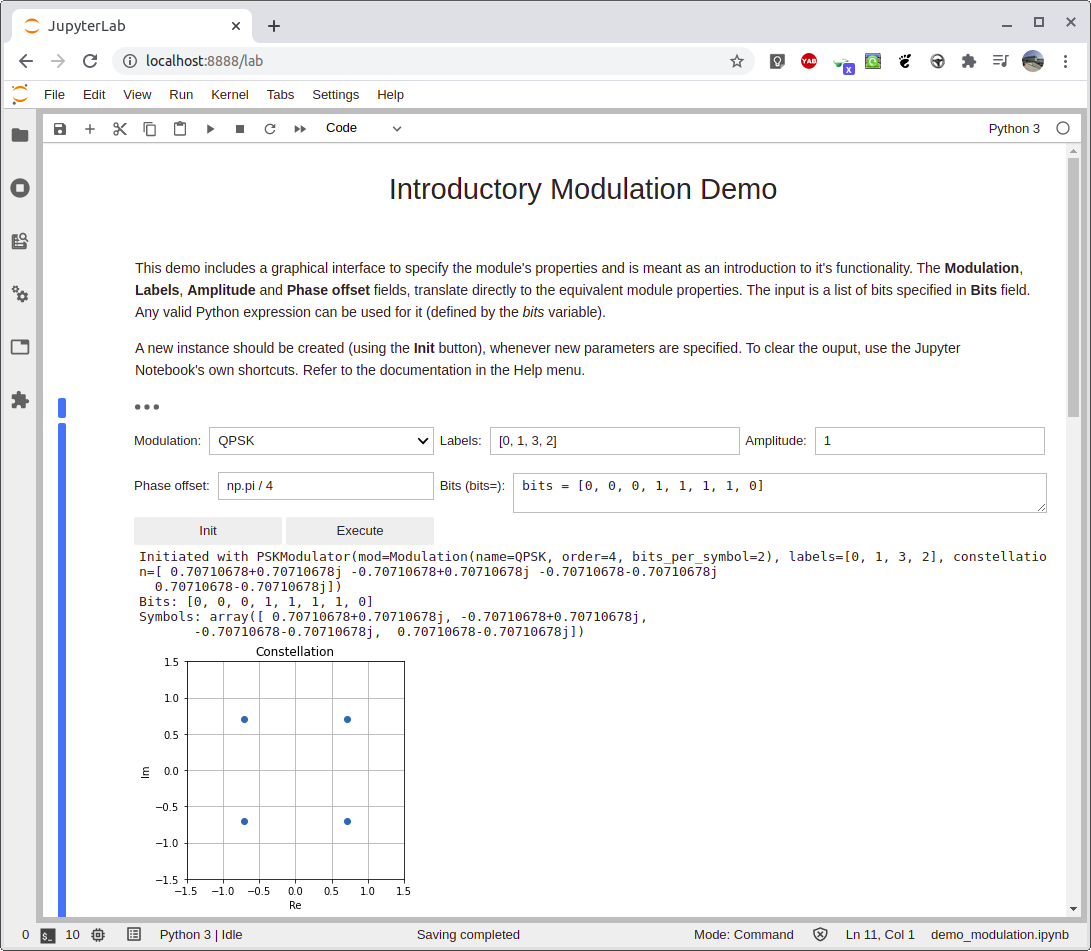
\includegraphics[width=0.75\textwidth]{demo_modulation}
  \caption{\code{PSKModulator} Jupyter notebook simple demonstration}
  \label{fig:demo_modulation}
\end{figure}

\begin{figure}[H]
  \centering
  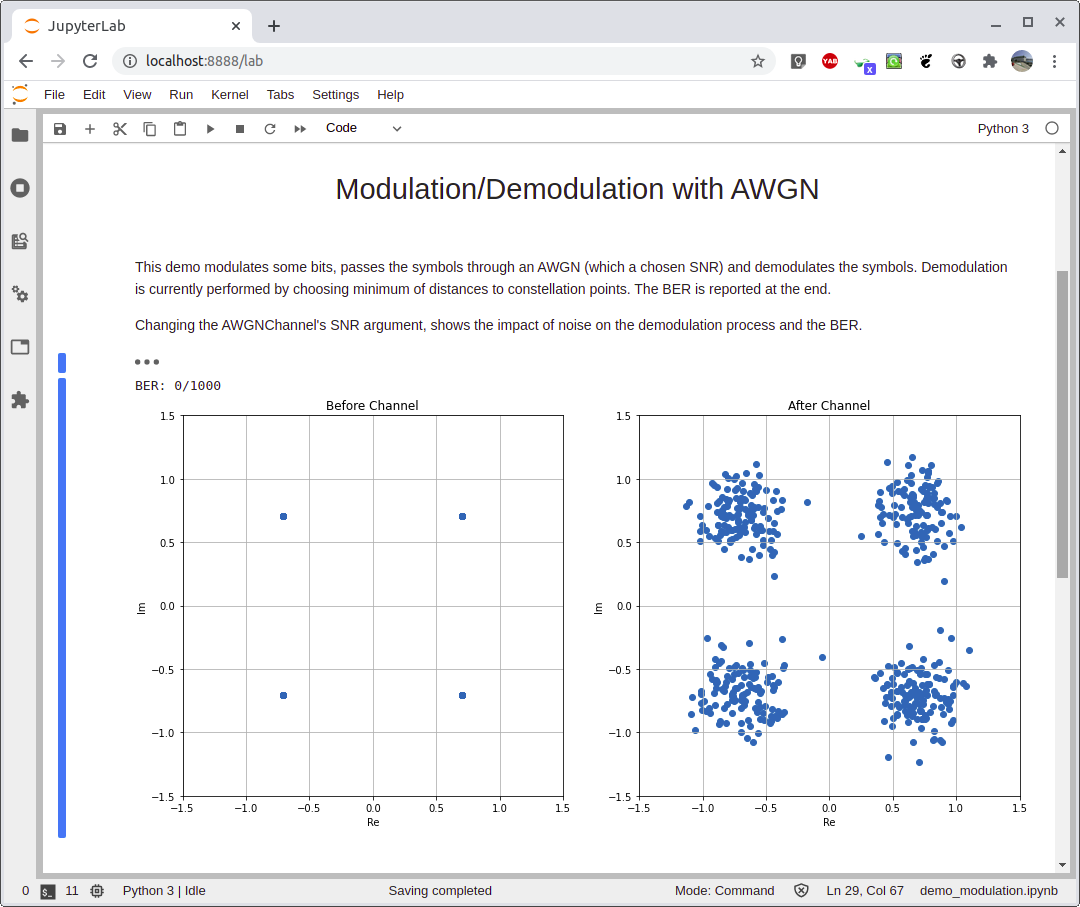
\includegraphics[width=0.75\textwidth]{demo_modulation2}
  \caption{\code{PSKModulator} Jupyter notebook demonstration with AWGN channel}
  \label{fig:demo_modulation2}
\end{figure}

%%%%%%%%%%%%%%%%%%%%%%%%%%%%%%%%%%%%%%%%%%%%%%%%%%%%%%%%%%%%%%%%%%%%%%%%%%%%%%%
\section{FIR Decimator/Interpolator}

To understand the decimation and interpolation processes, it's fundamental to grasp the concept of impulse-train sampling which simply means that samples of a discrete-time sequence $x(n)$ can be obtained by multiplying $x(n)$ by the sum of discrete-time impulse train positioned at the sampling instants $kN$, given by
\begin{align}
  p(n)=\sum_{k=-\infty}^{\infty}\delta(n-kN)
\end{align}
with DTFT
\begin{align}
  P(e^{j\Omega})=\frac{2\pi}{N}\sum_{k=-\infty}^{\infty}\delta\left(\Omega-k\frac{2\pi}{N}\right)
\end{align}

The desired sampled sequence is then:
\begin{align} \label{eq:x_pn}
  x_p(n) = x(n)p(n)
\end{align}
which is related to $x(n)$ by
\begin{align} \label{eq:x_p}
  x_p(n) =
  \begin{cases}
    x(n), & n=\text{integer} \times N\\
    0,    & \text{otherwise}\\
  \end{cases}
\end{align}

The DTFT of $x_p(n)$ can be obtained using frequency domain convolution and the sifting property for impulses:
\begin{align}
  X_p\left(e^{j\Omega}\right) &= \frac{1}{2\pi}\int_{-\pi}^{\pi}P\left(e^{j\theta}\right)X\left(e^{j\left(\Omega-\theta\right)}\right)d\theta \nonumber\\
                              &= \frac{1}{N}\sum_{k=0}^{N-1}X\left(e^{j\left(\Omega-k\frac{2\pi}{N}\right)}\right) \label{eq:X_p}
\end{align}

This result shows that sampling x$(n)$ by taking every $N$-th sample produces N copies of $X\left(e^{j\Omega}\right)$ evenly spaced in the interval $-\pi\leq\Omega\leq\pi$, with the amplitude of each copy scaled by $1/N$.

%%%%%%%%%%%%%%%%%%%%%%%%%%%%%%%%%%%%%%%
\subsection{Decimation}

The \code{FirDecimator} module filters and downsamples the input signal.

\noindent Module properties:
\begin{itemize}
  \item \code{factor}: Decimation factor
  \item \code{coeffs}: Filter coefficients
\end{itemize}

Downsampling the sequence $x(n)$ by $N$ is the process of decreasing the sampling rate by $N$ (where $N$ is specified using the \code{factor} property) by retaining the $N$-th sample of $x(n)$ to produce a new sequence $x_D(m)$. The $h_d(k)$ filter is needed to avoid aliasing, and its coefficients are provided in property \code{coeffs}. The process is illustrated in \autoref{fig:decimator}.

\begin{figure}[ht]
  \centering
  \includegraphics[width=0.75\textwidth]{decimator}
  \caption{Decimation by a factor $N$}
  \label{fig:decimator}
\end{figure}

The two sequences are related by
\begin{equation}
  x_D(m)=x(mN)
\end{equation}

Because only the $N$-th sample of $x(n)$ is of interest, $x_p(n)$, as given by \eqref{eq:x_pn}, could also be downsampled (at the proper starting point) to obtain the same sequence $x_D(m)$. The DTFT of $x_D(m)$ is then obtained as follows:
\begin{equation}
  X_D(e^{j\Omega}) = \sum_{m=-\infty}^{\infty} x_d(m)e^{-j\Omega m} = \sum_{m=-\infty}^{\infty} x_p(mN)e^{-j\Omega m}
\end{equation}

Substituting $m=n/N$, the summation can be re-expressed as
\begin{align}
  X_D(e^{j\Omega}) &= \sum_{n=\text{integer}\times N} x_p(n)e^{-j\Omega n/N} = \sum_{n=-\infty}^{\infty} x_p(n)e^{-j\Omega n/N} \nonumber\\
                   &= X_p(e^{j\Omega / N}) = \frac{1}{N} \sum_{k=0}^{N-1}X\left(e^j\left(\frac{\Omega-k2\pi}{N}\right)\right) \label{eq:X_D}
\end{align}

The relationship \eqref{eq:X_D} defines the following procedure to produce $X_D(e^{j\Omega})$ from $X(e^{j\Omega})$:
\begin{enumerate}
  \item Draw $N$ copies of $X(e^{j\Omega})$, each shifted by $2\pi k/N$ for $k=0,1,\ldots,N-1$
  \item Add the shifted copies together and scale the amplitude by $1/N$
  \item Stretch the frequency axis by $N$ by multiplying each of the `tick marks' on the frequency axis by $N$
\end{enumerate}

%%%%%%%%%%%%%%%%%%%%%%%%%%%%%%%%%%%%%%%
\subsection{Interpolation}

The \code{FirInterpolator} module upsamples and filters the input signal.

\noindent Module properties:
\begin{itemize}
  \item \code{factor}: Interpolation factor
  \item \code{coeffs}: Filter coefficients
\end{itemize}

Upsampling a sequence $x(n)$ by $N$ (where $N$ is specified using the \code{factor} property) is the process of increasing the sample rate by $N$ by inserting $N-1$ zeros between each sample of $x(n)$ to produce a new sequence $x_U(m)$. The filter $h_u(k)$ is needed for signal re-construction from the new samples, and its coefficients are provided in property \code{coeffs}. This process is illustrated in \autoref{fig:interpolator}.

\begin{figure}[ht]
  \centering
  \includegraphics[width=0.75\textwidth]{interpolator}
  \caption{Interpolation by a factor $N$}
  \label{fig:interpolator}
\end{figure}

The mathematical relationship between $x(n)$ and $x_U(m)$ is given by
\begin{equation}
x_U(m)=
  \begin{cases}
    x\left(\frac{m}{N}\right), & \text{$m=$ integer $\times$ $N$}\\
    0, & \text{otherwise}\\
  \end{cases}
\end{equation}

$X_U(m)$ looks like $x_p(m)$ from \eqref{eq:x_p}. In other words, if $x(n)$ is thought as the downsampled version of a fictitious high-rate $xx(m)$, then $x_U(m)$ can be viewed as the product $xx_p(m)=xx(m)p(m)$. Applying the relationship \eqref{eq:X_p} to $xx_p(m)$, it can be shown that the DTFT of the upsampled signal $x_U(m)$ is
\begin{equation}
X_U(e^{j\Omega})=XX_p(e^{j\Omega})=\frac{1}{N}\sum_{k-0}^{N-1} XX\left(e^{j\left(\Omega-k\frac{2\pi}{N}\right)}\right)
\end{equation}

Applying the downsampling results from \eqref{eq:X_D} , establishes the relationship between the DTFTs of and $xx(m)$ and $x(n)$:
\begin{equation}
X(e^{j\Omega})=\frac{1}{N}\sum_{k-0}^{N-1} XX\left(e^{j\left(\frac{\Omega-k2\pi}{N}\right)}\right)\implies X(e^{j\Omega N})=\frac{1}{N}\sum_{k-0}^{N-1} XX\left(e^{j\left(\Omega-k\frac{2\pi}{N}\right)}\right)
\end{equation}

Putting these results together gives the desired relationship:
\begin{equation}
X_U(e^{j\Omega})=X(e^{j\Omega N})
\end{equation}

This relationship defines the following procedure to produce $X_U(e^{j\Omega})$ from $X(e^{j\Omega})$:
\begin{enumerate}
  \item Starting with $X(e^{j\Omega})$, compress the frequency axis by $N$ by dividing all the `tick marks' on the frequency axis by $N$
  \item Draw $N-1$ shifted copies of the compressed spectrum. Each copy is shifted by $2\pi k/N$, for $k=0,1,\ldots,N-1$
\end{enumerate}

In other words, the result shows that $N$ copies of the compressed spectrum of $x(n)$ alias into the first Nyquist zone.

\autoref{fig:demo_interpolator} and \autoref{fig:demo_interpolator2} show a Jupyter notebook interface and execution for a demonstration of the \code{FirInterpolator} module. Note that the output signal (the orange trace) has a delay corresponding to 20 samples, which is $(L-1)/2$ where $L$ is the length of the interpolation filter (41 in the example shown). The filter is a \emph{square-root raised cosine} (RRC) filter with a span of 10 symbols, 4 samples per symbol, and roll off factor of 0.5.

\begin{figure}[H]
  \centering
  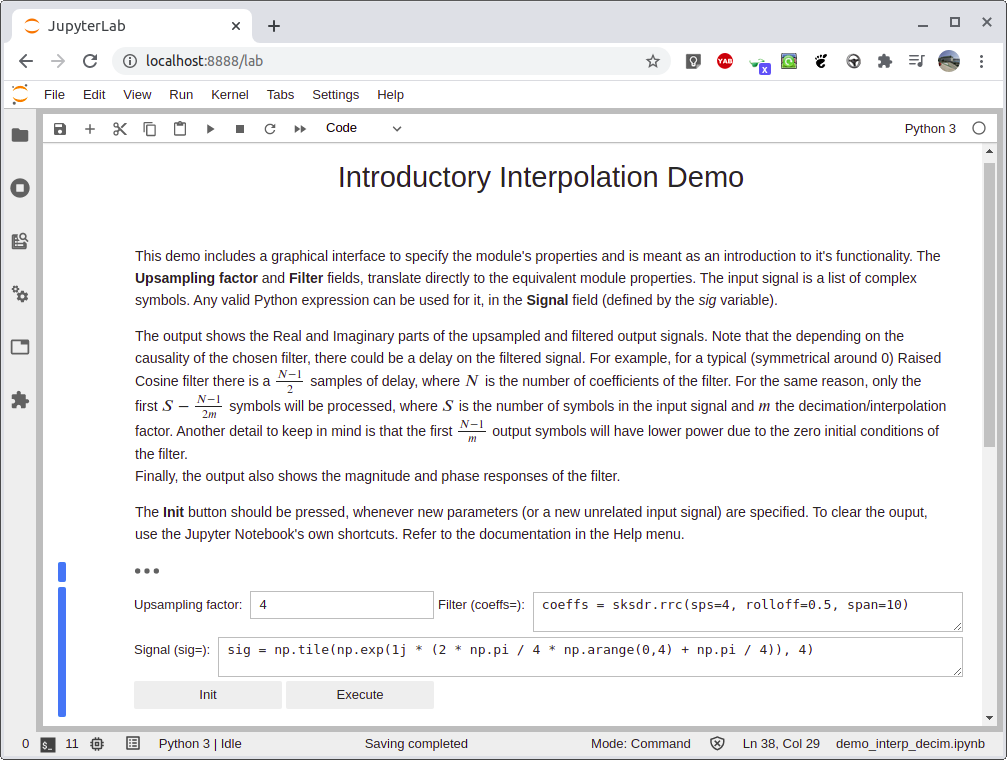
\includegraphics[width=0.75\textwidth]{demo_interpolator}
  \caption{\code{FirInterpolator} Jupyter notebook demonstration interface}
  \label{fig:demo_interpolator}
\end{figure}

\begin{figure}[H]
  \centering
  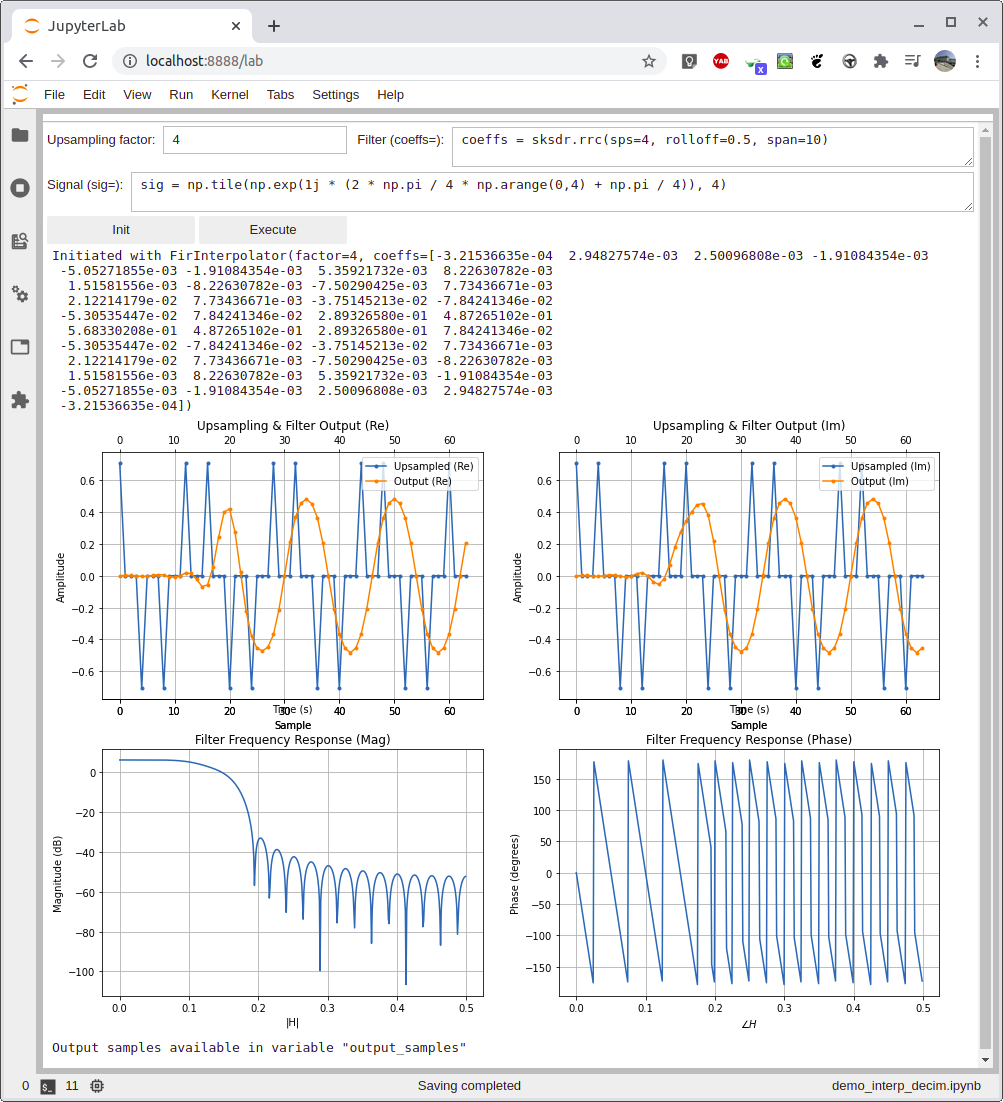
\includegraphics[width=0.75\textwidth]{demo_interpolator2}
  \caption{\code{FirInterpolator} Jupyter notebook demonstration results}
  \label{fig:demo_interpolator2}
\end{figure}

%%%%%%%%%%%%%%%%%%%%%%%%%%%%%%%%%%%%%%%%%%%%%%%%%%%%%%%%%%%%%%%%%%%%%%%%%%%%%%%
\section{Coarse Frequency Compensator}

The \code{CoarseFrequencyComp} module performs an open loop frequency correction to a PSK input signal.

\noindent Module properties:
\begin{itemize}
  \item \code{mod\_order}: Modulation order (e.g., 2 for BPSK, 4 for QPSK)
  \item \code{sample\_rate} (Hz): Input signal sampling rate
  \item \code{freq\_res} (Hz): Desired frequency resolution
\end{itemize}

The algorithm estimates the frequency error $\Delta\hat{f}$ by using a periodogram of the $m^{th}$ power of the received signal (the $m^{th}$ power is used since it removes the $m^{th}$ order PSK modulation, leaving only the carrier at a frequency $m$ times its original frequency):
\begin{equation}
\Delta\hat{f}=\frac{f_s}{m\cdot N}\underset{f}{\operatorname{argmax}}\left|\sum_{n=0}^{N-1} r(n)^m e^{-j\frac{2\pi k}{N}n}\right|
\end{equation}
where $f_s$ is the sampling frequency (specified by \code{sample\_rate}), $m$ is the modulation order (specified by \code{mod\_order}), $r(n)$ is the received sequence, and $N$ is the number of samples of the periodogram. To avoid aliasing $\Delta\hat{f}$ must be restricted to $\left[\frac{-R_{sym}}{2}, \frac{R_{sym}}{2}\right]$, where $R_{sym}=\frac{R_b}{log_2(m)}$, with $R_b$ representing the bit rate.

The algorithm effectively searches for a frequency that maximizes the time average of the $m^{th}$ power of the received signal multiplied by frequencies in the range of $\left[\frac{-R_{sym}}{2}, \frac{R_{sym}}{2}\right]$. As the form of the algorithm is the definition of the DFT of $r^{m}(n)$, searching for a frequency that maximizes the time average is equivalent to searching for a peak line in the spectrum of $r^{m}(n)$. The number of points required by the FFT is
\begin{equation}
  N=2^{log_2\left(\frac{f_s}{f_r}\right)}
\end{equation}
where $f_r$ is the desired frequency resolution, specified by \code{freq\_res}. Note that $log_2\left(\frac{f_s}{f_r}\right)$ should be rounded up, since it might not be integer.

\autoref{fig:demo_cfc} shows a Jupyter notebook with a demonstration of the \code{CoarseFrequencyComp} module. One can observe that the output signal's spectrum has been shifted, in order to correct the introduced frequency offset.

\begin{figure}[H]
  \centering
  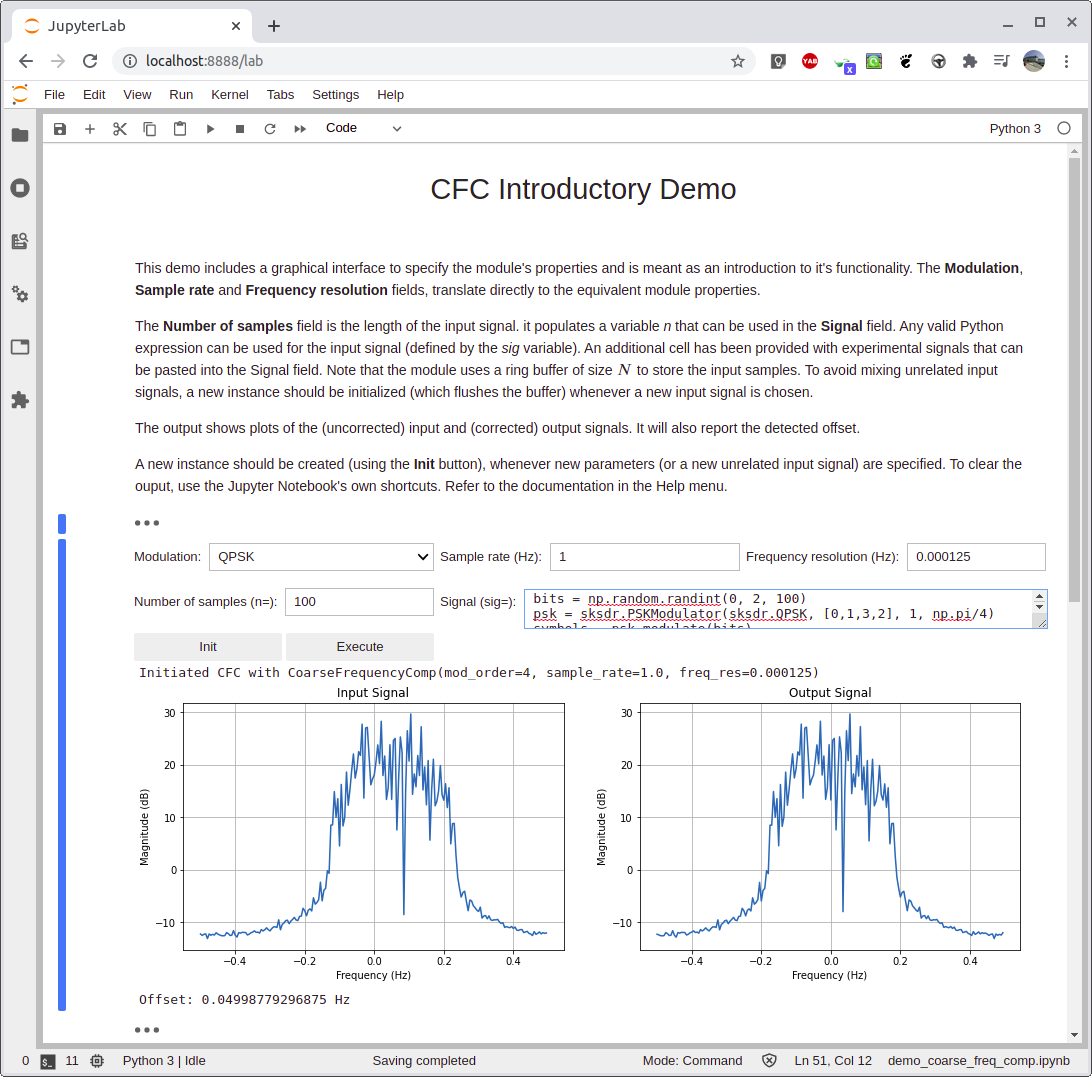
\includegraphics[width=0.75\textwidth]{demo_cfc}
  \caption{\code{CoarseFrequencyComp} Jupyter notebook demonstration}
  \label{fig:demo_cfc}
\end{figure}

%%%%%%%%%%%%%%%%%%%%%%%%%%%%%%%%%%%%%%%%%%%%%%%%%%%%%%%%%%%%%%%%%%%%%%%%%%%%%%%
\section{Carrier Frequency Synchronizer (with an introduction to PLLs)}
\label{sect:library_freq_sync}

The \code{FrequencySync} module compensates for carrier frequency and phase offsets in signals that use single-carrier modulation schemes. Currently it supports BPSK and QPSK.

\noindent Module properties:
\begin{itemize}
  \item \code{sps}: Samples per symbol of the input signal
  \item \code{mod}: Modulation of the input signal
  \item \code{damp\_factor}: PLL's damping factor
  \item \code{norm\_loop\_bw}: PLL's normalized loop bandwidth
\end{itemize}

\subsection{Phase-locked Loop Introduction}
\label{sect:pll_intro}
The module is a closed loop synchronizer that uses the discrete phase-locked loop (PLL) based algorithm described in \cite{digcomm_discrete_approach}. PLLs are often used in digital communications to synchronize local oscillators in the receiver to oscillators used in the transmitter (carrier phase synchronization) or to synchronize the data clock in the receiver to the transmitter data clock (symbol timing synchronization). In either case, the PLL can be though as a device that tracks the phase and frequency of a sinusoid. A basic structure of a PLL is shown in \autoref{fig:analog_pll}.

\begin{figure}[ht]
  \centering
  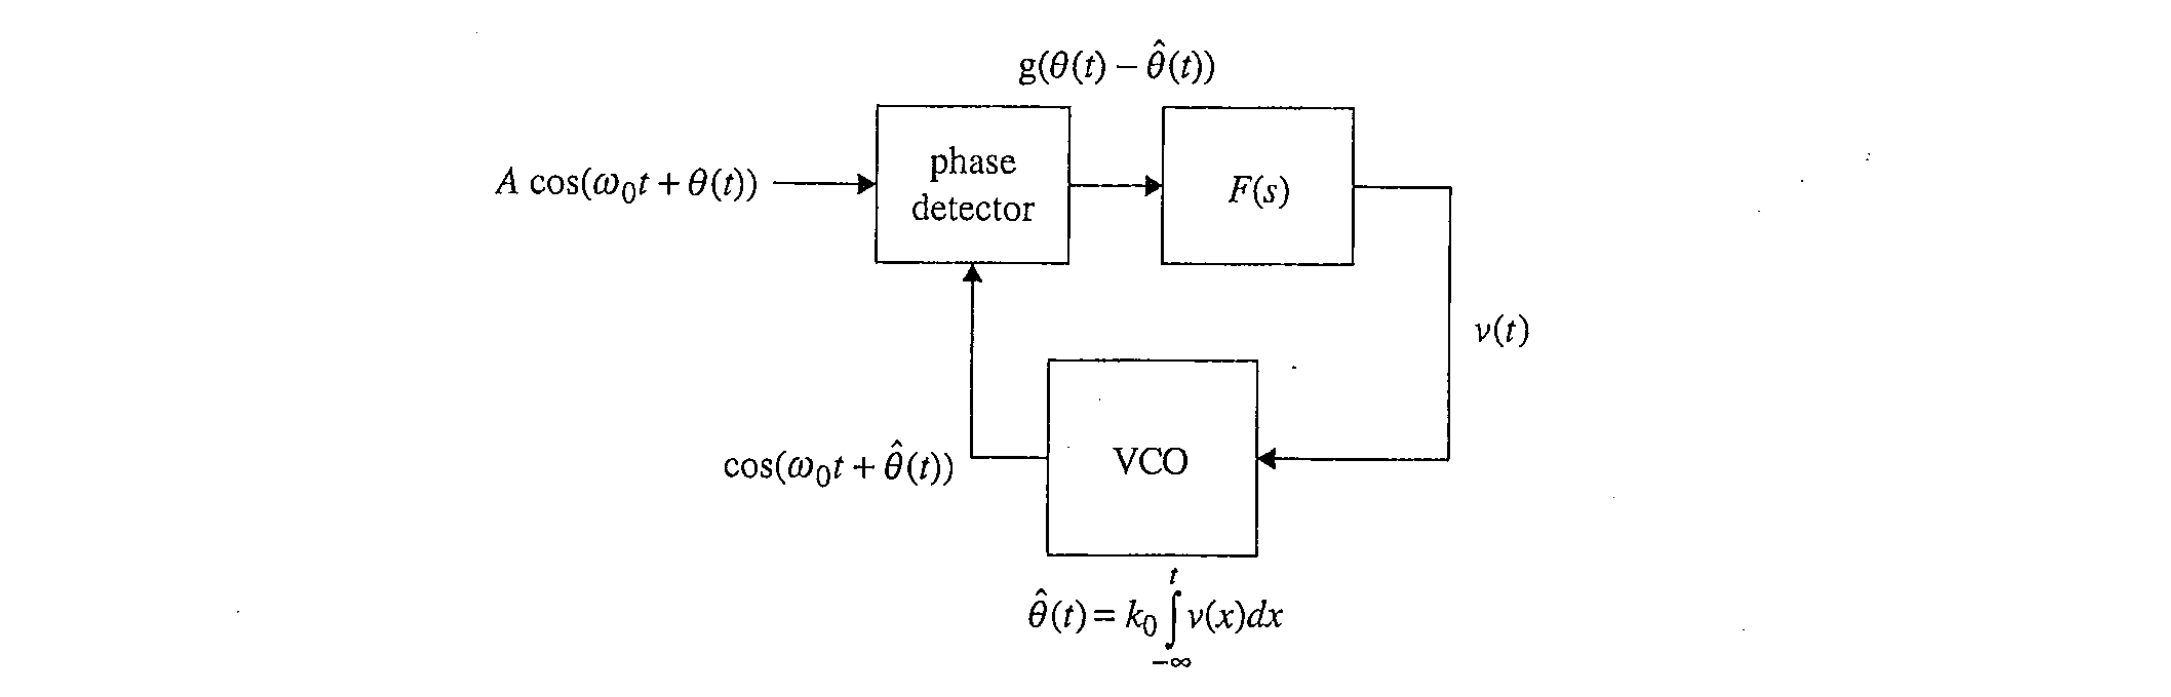
\includegraphics[width=\textwidth]{analog_pll}
  \caption{Basic structure of phase locked loop [\citeauthor{digcomm_discrete_approach}]}
  \label{fig:analog_pll}
\end{figure}

It's also common to produce a \emph{phase equivalent} representation writing down the phases of all sinusoids and tracking the operations on those phases through the PLL. This structure is illustrated in \autoref{fig:analog_pll_phases}.

\begin{figure}[ht]
  \centering
  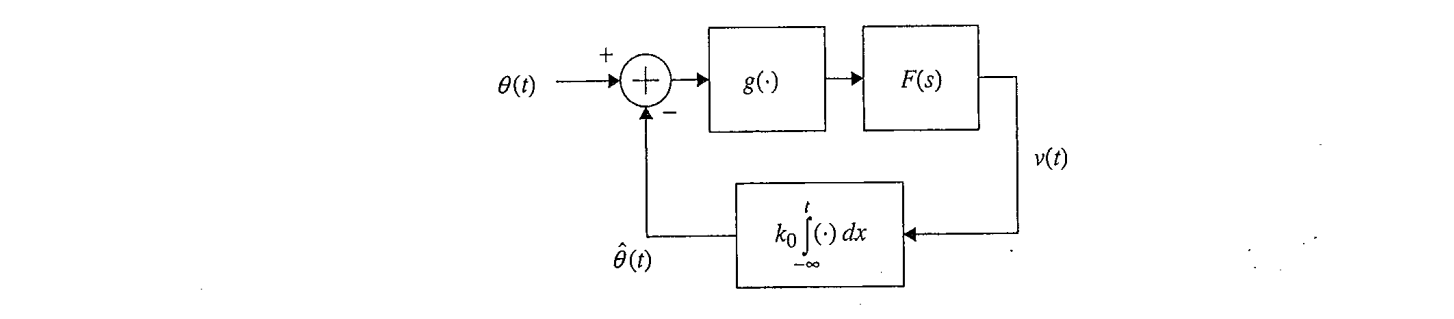
\includegraphics[width=\textwidth]{analog_pll_phases}
  \caption{Phase equivalent PLL corresponding to the PLL in \autoref{fig:analog_pll} [\citeauthor{digcomm_discrete_approach}]}
  \label{fig:analog_pll_phases}
\end{figure}

The system is composed of three blocks: the phase detector, the loop filter and the voltage-controlled oscillator (VCO). The loop input $\theta(t)$ and the VCO output $\hat\theta(t)$ are the inputs to the phase detector, and the difference in phase between these inputs is known as the \emph{phase error} $\theta_e(t)=\theta(t) -\hat\theta(t)$. The output of the phase detector is a function of this phase error $g(\theta_e)$. This, in turn, is filtered by the loop filter to produce an input to the VCO which controls its output phase. When functioning correctly, the loop adjusts the control voltage $v(t)$ to produce a phase estimate $\hat\theta(t)$ that drives the phase error to zero. \autoref{fig:s-curve} shows the plot of the phase detector output $g(\theta_e(t)$. When the phase error is positive, $\theta(t) > \hat \theta(t)$, which means the phase of the VCO output lags the loop input and must be increased. The phase error produces a control input voltage $v(t)$ on the VCO, which in turn increases its output phase, producing the desired results. When the phase error is negative, $\theta(t) < \hat \theta(t)$, a negative control voltage is produced and the VCO decreases its output phase.

\begin{figure}[ht]
  \centering
  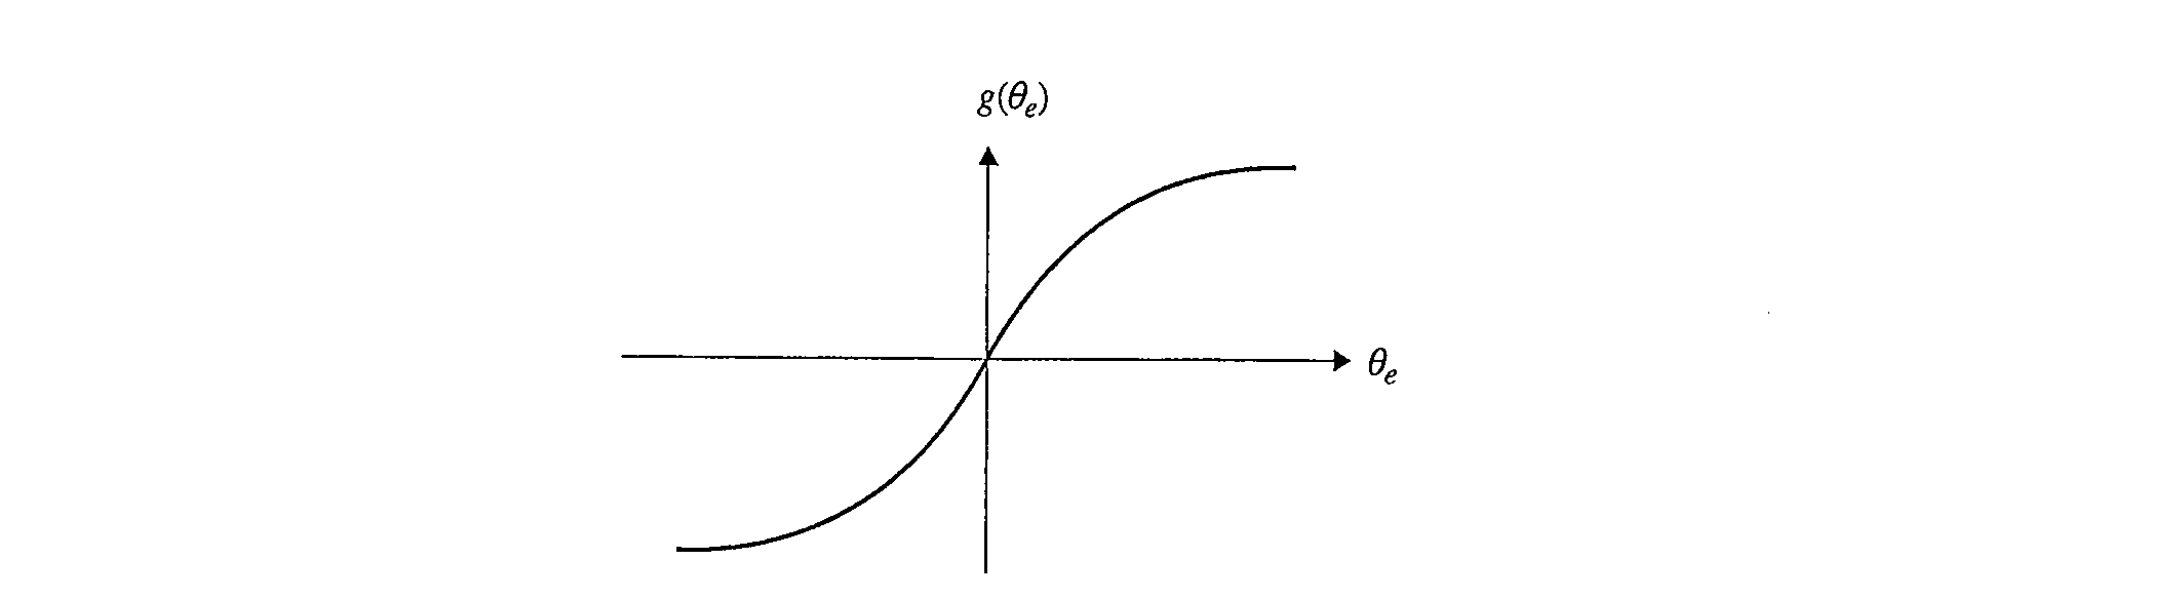
\includegraphics[width=\textwidth]{s-curve}
  \caption{Typical phase detector input-output curve known as an `S curve' [\citeauthor{digcomm_discrete_approach}]}
  \label{fig:s-curve}
\end{figure}

To derive the system parameters we can start with an analogue PLL structure and then obtain the equivalent parameters in the digital domain.

Given that the phase detector can be a non-linear function, a common method of analysing these systems is to linearize them around a desired operation point (in this case $\theta_e=0$). The linear approximation is obtained by considering that $g(\theta_e)\approx k_p \theta_e$, for small $\theta_e$. Having a linear system, the phase equivalent diagram can now be analysed using frequency domain techniques (Laplace or Z transforms) to extract the parameters that characterize the properties and performance of the system. \autoref{fig:analog_pll_linear} shows the linearized system in the time and frequency domains.

\begin{figure}[ht]
  \centering
  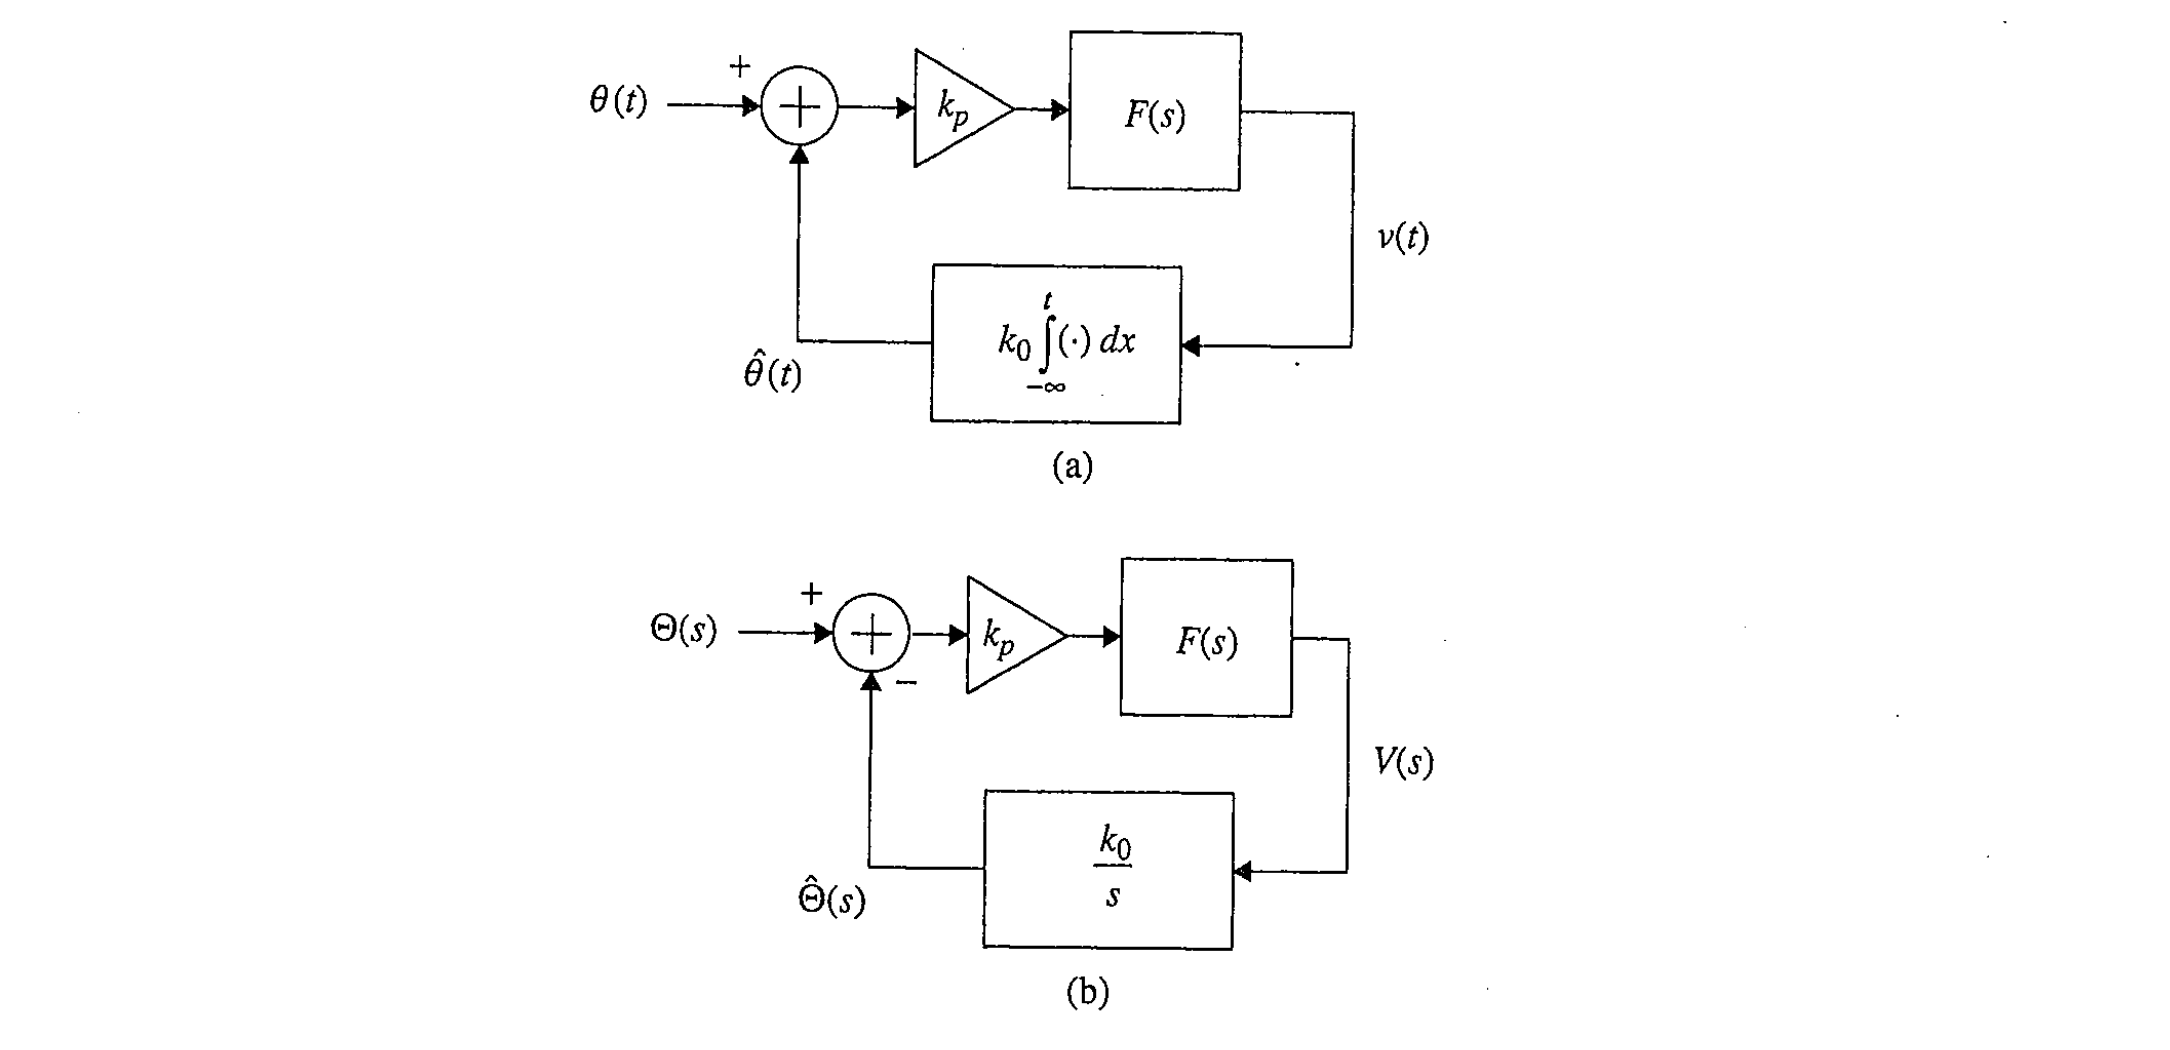
\includegraphics[width=\textwidth]{analog_pll_linear}
  \caption{Linearized equivalent, both in time and frequency domains, of the PLL show in \autoref{fig:analog_pll} [\citeauthor{digcomm_discrete_approach}]}
  \label{fig:analog_pll_linear}
\end{figure}

Two particular input signals (the phase step input (corresponding to a constant phase offset: $\theta(t) = \Delta\theta\cdot u(t)$) and the phase ramp input (corresponding to a constant frequency offset: $\theta(t) = (\Delta \omega)t\cdot u(t)$)) are used to analyse the \emph{phase error response}. The transfer function for the phase error detector is
\begin{equation}
  G(s)=\frac{\Theta_e(s)}{\Theta(s)}=\frac{s}{s+k_0 k_p F(s)}
\end{equation}

replacing the Laplace transforms of the step and ramp inputs (respectively $\Theta_{step}(s)=\frac{\Delta \theta}{s}$ and $\Theta_{ramp}(s)=\frac{\Delta \omega}{s^2}$) into that expression, allows obtaining the phase error responses:
\begin{align}
\Theta_{e,step}(s) & =\frac{\Delta\theta}{s+k_0 k_p F(s)}\\
\Theta_{e,ramp}(s) & =\frac{\Delta\omega}{s^2+s k_0 k_p F(s)}
\end{align}

applying the final value theorem one extracts the conditions on the loop filter:
\begin{align}
\theta_{e,step}(\infty) & =\lim_{s\to 0}\left(s\cdot\Theta_{e,step}(s)\right)=0\text{, if }F(0)\neq0\\
\theta_{e,ramp}(\infty) & =\lim_{s\to 0}\left(s\cdot\Theta_{e,ramp}(s)\right)=0\text{, if }F(0)=\infty
\end{align}

It can be seen that to force the phase error $\theta_e$ to 0, the loop must have a non-zero DC gain (condition imposed by the step response), and an infinite DC gain (condition imposed by the ramp response). A \emph{proportional-plus-integrator} has these properties. Notice that while it's difficult to implement an infinite DC gain integrator in the analogue domain, it is straightforward in the digital domain and so this is the chosen structure for the loop filter:
\begin{equation}F(s)=k_1+\frac{k_2}{s}\end{equation}

To extract the loop performance in turn, the \emph{output response} is analysed:
\begin{equation}H_a(s)=\frac{\hat\Theta(s)}{\Theta(s)}=\frac{k_0 k_p F(s)}{s+k_0 k_p F(s)}\end{equation}

With $F(s)$ as a proportional-plus-integrator loop filter, this becomes
\begin{equation}H_a(s)=\frac{\hat\Theta(s)}{\Theta(s)}=\frac{k_0 k_p k_1 s + k_0 k_p k_2}{s^2+k_0 k_p k_1 s + k_0 k_p k_2}\end{equation}

This is a second order system (it has two poles, one originating from the loop filter and the other from the VCO) and so it can be expressed in the familiar form
\begin{equation} \label{eq:Ha_s}
  H_a(s)=\frac{2\zeta \omega_n s+\omega_n^2}{s^2+2\zeta \omega_n s+\omega_n^2}
\end{equation}
where
\begin{align}
\zeta & =\frac{k_1}{2}\sqrt{\frac{k_0 k_p}{k_2}}\\
\omega_n & = \sqrt{k_0 k_p k_2}
\end{align}
are the \emph{damping factor} and \emph{natural frequency} of the system.

Sometimes it's common to specify the 3-dB bandwidth of the PLL $\omega_{3dB}$, obtained by setting $|H_a(j\omega)|^2=\frac{1}{2}$ and solving for $\omega$. In this case
\begin{equation}\omega_{3dB}=\omega_n \sqrt{1+2\zeta^2+\sqrt{(1+2\zeta^2)^2+1}}\end{equation}

While this maybe a familiar concept, $\omega_{3dB}$ is not very useful as a measure of the bandwidth of a PLL, so an alternative parameter is $B_n$, the \emph{equivalent noise bandwidth}, defined as the bandwidth of a fictitious rectangular low-pass filter with the same area as $|H_a(j\omega)|^2$. With a proportional-plus-integrator filter, this turns out to be
\begin{equation}B_n=\frac{\omega_n}{2}\left(\zeta+\frac{1}{4\zeta}\right)\end{equation}

With equations for $\zeta$, $\omega_n$ and $B_n$, it's possible, in turn, to obtain expressions for the loop constants:
\begin{align}
k_p k_0 k_1 &= \frac{4\zeta B_n}{\zeta+\frac{1}{4\zeta}}\\
k_p k_0 k_2 &= \frac{4 B_n^2}{\left(\zeta+\frac{1}{4\zeta}\right)^2}
\end{align}

With this analysis, one is now in the position to derive the equivalent discrete-time PLL structure. Using the bilinear transform, it's possible obtain the corresponding discrete-time PLL parameters. \autoref{fig:discrete_pll_basic_and_phases} shows the basic structure of a discrete-time PLL and the corresponding phase equivalent PLL.

\begin{figure}[ht]
  \centering
  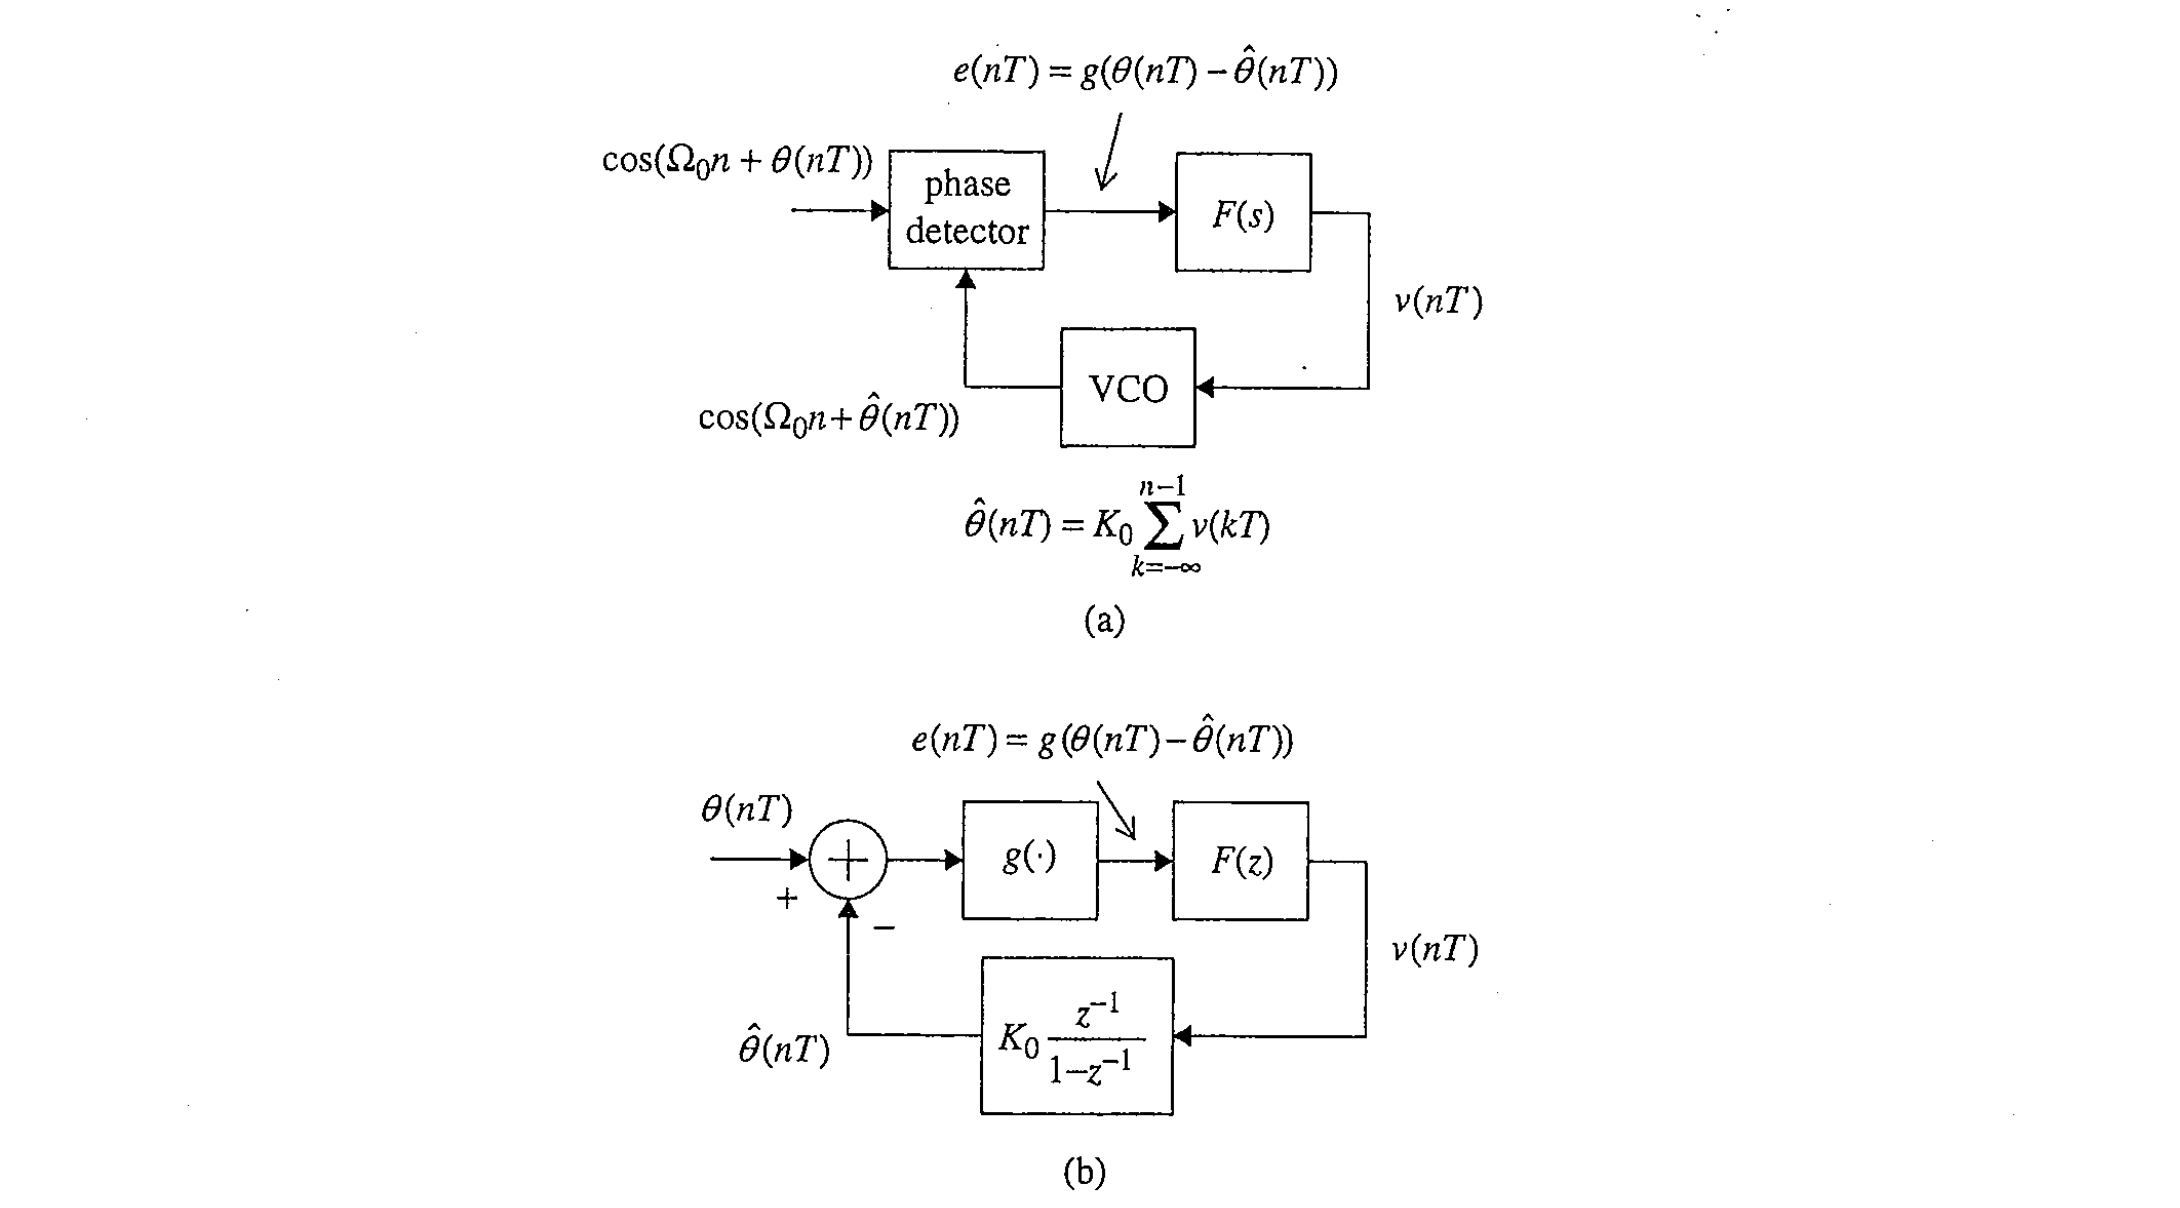
\includegraphics[width=\textwidth]{discrete_pll_basic_and_phases}
  \caption{Basic structure of a discrete-time PLL a) and the corresponding phase equivalent PLL b) [\citeauthor{digcomm_discrete_approach}]}
  \label{fig:discrete_pll_basic_and_phases}
\end{figure}

If one introduces in the general block diagram of a PLL, the assumptions made (a constant phase detector gain $k_p$ and the a proportional-plus-integrator filter), then the detailed linearized structure of both the PLL and its phase equivalent emerges, and is shown in \autoref{fig:analog_pll_pplus_int_and_linear_phase_equiv} for the continuous-time case, and in \autoref{fig:digital_pll_pplus_int_and_linear_phase_equiv} for the discrete-time case. The direct digital synthesizer (DDS) is the discrete-time equivalent of the VCO. These two figures serve as a useful reference for the following derivation of the discrete-time PLL parameters.

\begin{figure}[H]
  \centering
  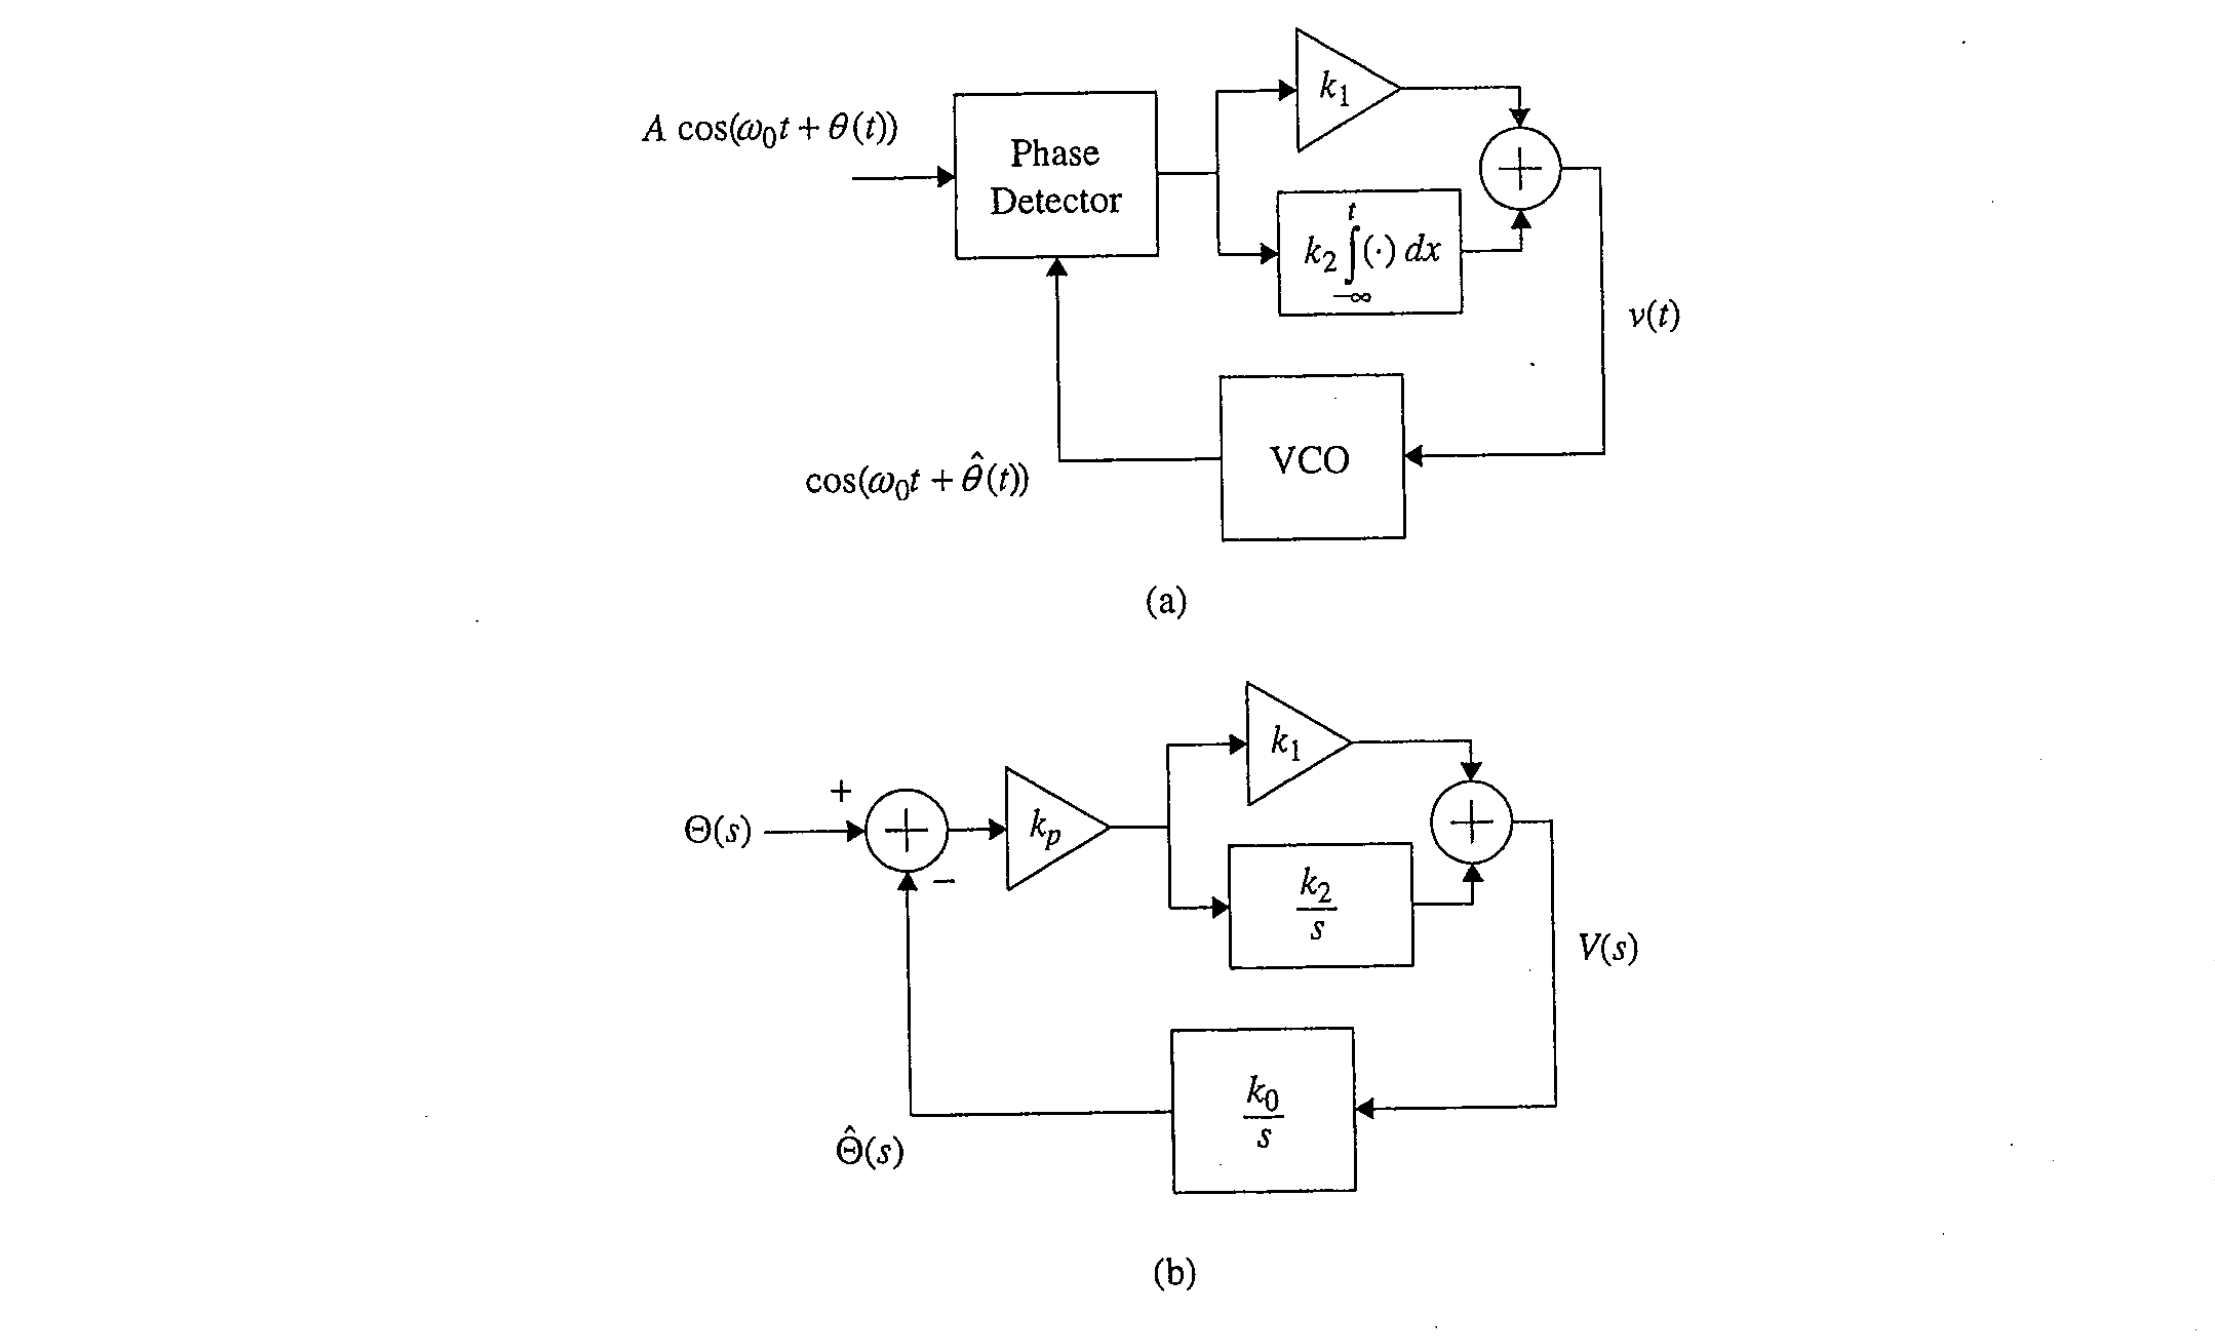
\includegraphics[width=\textwidth]{analog_pll_pplus_int_and_linear_phase_equiv}
  \caption{Second-order continuous-time phase locked loop with proportional-plus-integrator loop filter (a) and the linearized phase equivalent PLL (b) [\citeauthor{digcomm_discrete_approach}]}
  \label{fig:analog_pll_pplus_int_and_linear_phase_equiv}
\end{figure}

\begin{figure}[H]
  \centering
  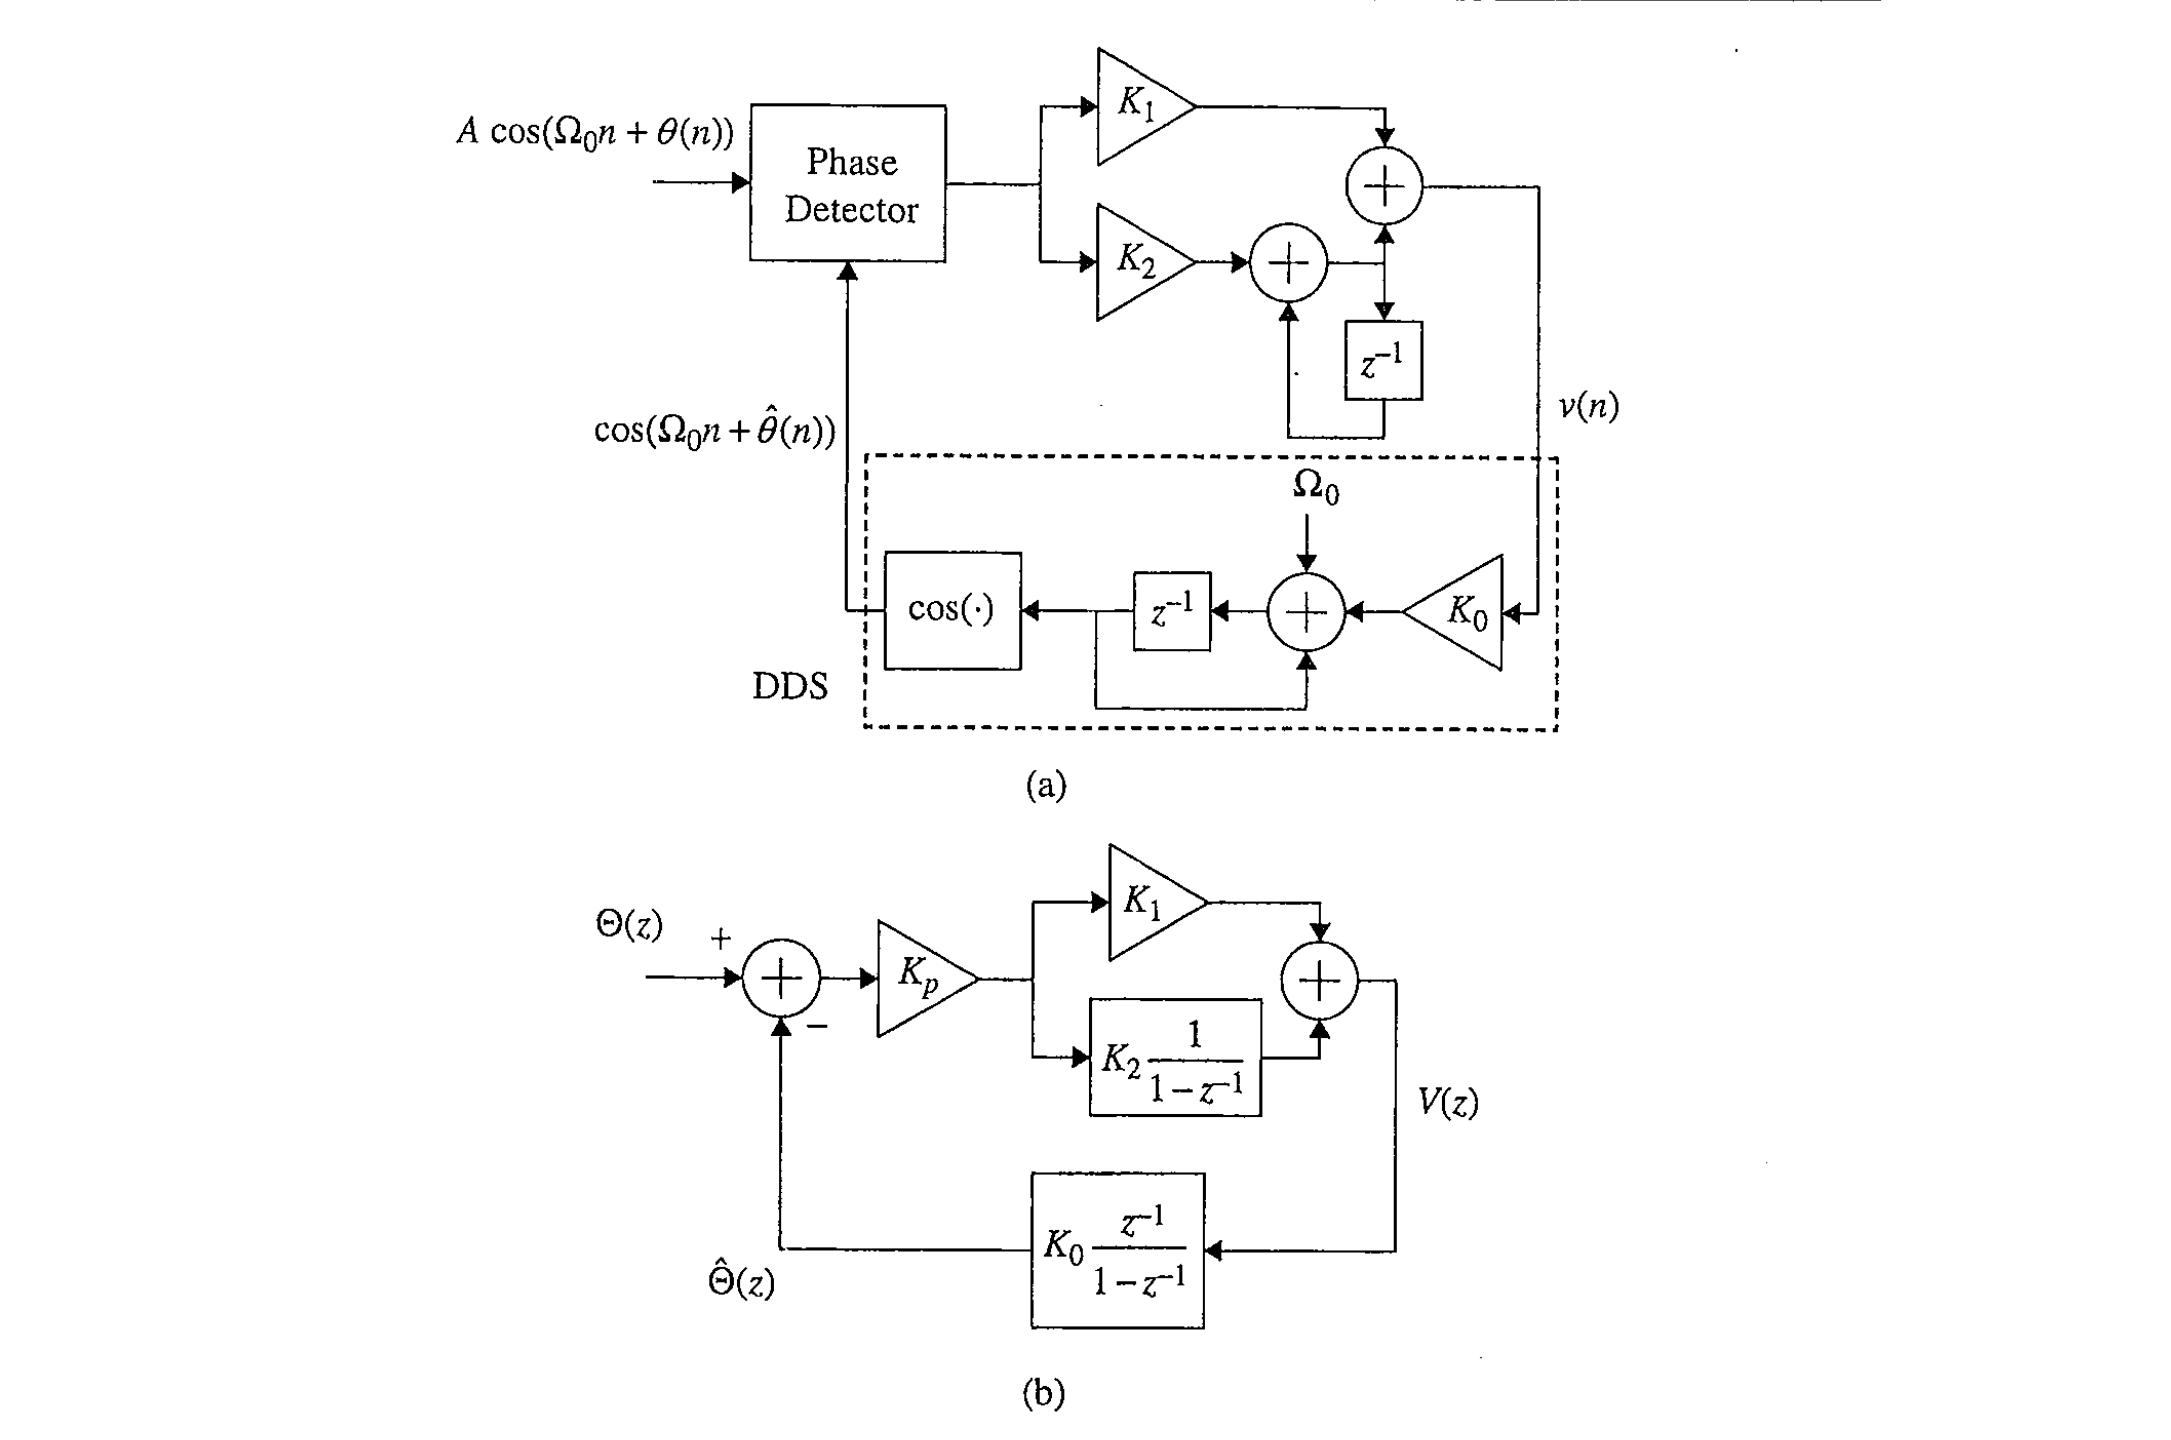
\includegraphics[width=\textwidth]{digital_pll_pplus_int_and_linear_phase_equiv}
  \caption{Second-order discrete-time phase locked loop with proportional-plus-integrator loop filter  that mimics the continuous-time PLL in \autoref{fig:analog_pll_pplus_int_and_linear_phase_equiv} (a) and the linearized phase equivalent discrete-time PLL (b) [\citeauthor{digcomm_discrete_approach}]}
  \label{fig:digital_pll_pplus_int_and_linear_phase_equiv}
\end{figure}

One already knows the continuous output response from \eqref{eq:Ha_s}. From \autoref{fig:digital_pll_pplus_int_and_linear_phase_equiv} it is possible to derive the discrete-time equivalent:
\begin{equation}H_d(z)=\frac{K_p K_0 (K_1+K_2)z^{-1}-K_p K_0 K_1 z^{-2}}{1-2\left(1-\frac{1}{2}K_p K_0 \left(K_1+K_2\right)
\right)z^{-1}+\left(1-K_p K_0 K_1 \right)z^{-2}}\end{equation}

Applying Tustin's equation (bilinear transform) to $H_a(s)$ produces $H_a\left(\frac{2}{T}\frac{1-z^{-1}}{1+z^{-1}}\right)$. Equating and rearranging the denominators of $H_a\left(\frac{2}{T}\frac{1-z^{-1}}{1+z^{-1}}\right)$ and $H_d(z)$, and solving for the loop constants finally produces
\begin{align}
K_p K_0 K_1 &= \frac{4\zeta\theta_n}{1+2\zeta\theta_n+\theta_n^2}\\
K_p K_0 K_2 &= \frac{4\theta_n^2}{1+2\zeta\theta_n+\theta_n^2}
\end{align}
where
\begin{equation}\theta_n=\frac{\omega_n T}{2}\end{equation}
which can be re-expressed in terms of $B_n$ and $\zeta$, given the relations obtained in the proportional-plus-integrator loop filter case:
\begin{equation}\theta_n=\frac{B_n T}{\zeta+\frac{1}{4\zeta}}=\frac{B_n T_s}{N\left(\zeta+\frac{1}{4\zeta}\right)}\end{equation}
where $T$ is the sampling period, $T_s$ the symbol period and $N$ the number of samples per symbol.

Replacing this in the loop constant equations gives
\begin{align}
K_p K_0 K_1 &= \frac{4\zeta\left(\frac{B_n T_s}{N\left(\zeta+\frac{1}{4\zeta}\right)}\right)}{1+2\zeta\left(\frac{B_n T_s}{N\left(\zeta+\frac{1}{4\zeta}\right)}\right)+\left(\frac{B_n T_s}{N\left(\zeta+\frac{1}{4\zeta}\right)}\right)^2}\\
K_p K_0 K_2 &= \frac{4\left(\frac{B_n T_s}{N\left(\zeta+\frac{1}{4\zeta}\right)}\right)^2}{1+2\zeta\left(\frac{B_n T_s}{N\left(\zeta+\frac{1}{4\zeta}\right)}\right)+\left(\frac{B_n T_s}{N\left(\zeta+\frac{1}{4\zeta}\right)}\right)^2}
\end{align}
which, when, as often is the case, $B_nT\ll1$, can be approximated as
\begin{align}
\label{eq:digital_loop_constants1} K_p K_0 K_1 &\approx \frac{4\zeta}{\zeta+\frac{1}{4\zeta}}\frac{B_n T_s}{N}\\
\label{eq:digital_loop_constants2} K_p K_0 K_2 &\approx \frac{4}{\left(\zeta+\frac{1}{4\zeta}\right)^2}\left(\frac{B_n T_s}{N}\right)^2
\end{align}

Note that, in this approximation, where the sample rate is large relative to the equivalent loop bandwidth, the discrete-time expressions are the same as those for the continuous-time loop case, except that the loop bandwidth is normalized by the sample rate (or the symbol rate).

\subsection{PLL design for PSK carrier frequency synchronization}
Up until this point, the structure of a general discrete-time PLL has been derived, with the exception of the phase error detector, which has been assumed only to be linear, more specifically $g(\theta_e)=K_p\theta_e$. Unfortunately this general case does not work for the specific case of PSK modulations because if this PLL was applied to the input signal it would try to track both the carrier phase error and the phase offsets introduced by the modulation itself. Thus the PLL must \emph{remove} the modulation phase shifts and track only the remaining phase. The \emph{maximum likelihood} (ML) phase error detector is chosen instead, which consists of minimizing the energy in $\theta_e$. It also has the advantage of avoiding arctangent operations required by other phase detectors based on a purely geometric approach. \autoref{fig:complete_digital_pll} shows the complete discrete-time PLL (for QPSK modulation case) with the proposed ML phase error detector.
\begin{figure}[ht]
  \centering
  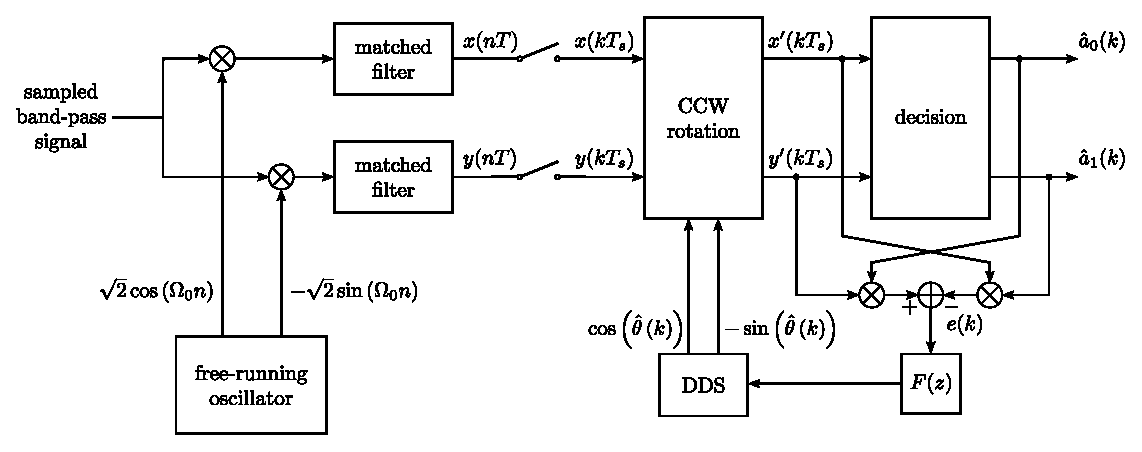
\includegraphics[width=\textwidth]{drawing}
  \caption{Block diagram for the QPSK carrier phase PLL using an error signal based on the ML phase error detector}
  \label{fig:complete_digital_pll}
\end{figure}
The ML phase detector first de-rotates the input signal by the estimated phase from the DDS output (CCW rotation block). This leaves only the phase of the received data symbol $\theta_r = \theta-\hat\theta$. It then subtracts the phase of the transmitted data symbol to obtain the phase error, $\theta_e=\theta_r-\theta_d$. This is usually used in a \emph{data-aided} system, in which there is a training sequence where the transmission symbols are well known. If the symbols are unknown then it is called a \emph{decision-directed} system and the transmitted symbols must be estimated. In that case, $\theta_e$ is more accurately denoted by $\theta_e=\theta_r-\hat\theta_d$. The latter is the situation in this case. It can be shown \cite{digcomm_discrete_approach} that the ML phase detector response is given by
\begin{align}
  e(k)=y'(kT_s)\hat a_0(k)-x(kT_s)'\hat a_1(k)
\end{align}

For QPSK the decisions are
\begin{align}
\hat a_0(k) &= A\times\operatorname{sgn}\left[x(kT_s)'\right] \\
\hat a_1(k) &= A\times\operatorname{sgn}\left[y(kT_s)'\right]
\end{align}

Expressing $x'(kT_s)$ and $y'(kT_s)$ in terms of $\theta_e$, $a_0(k)$ and $a_1(k)$, and averaging over all four possible symbols, produces the S-curve for the ML phase error detector for the data-aided case:
\begin{align}
\overline{g}_{\text{QPSK}}(\theta_e) &= 2KA^2\sin(\theta_e)\approx 2KA^2\theta_e\text{, for }\theta_e\approx0\\
\overline{g}_{\text{BPSK}}(\theta_e) &= KA^2\sin(\theta_e)\approx KA^2\theta_e\text{, for }\theta_e\approx0
\end{align}
where $K$ is the amplitude of the received signal and $A$ is the norm of symbols. This gives the desired $K_p$:
\begin{align}
K_{p_{\text{QPSK}}} &= 2KA^2\\
K_{p_{\text{BPSK}}} &= KA^2
\end{align}

The decision-directed case, is given by
\begin{align}
  \overline{g}_{\text{QPSK}}(\theta_e)=
    \begin{cases}
      -2KA^2 \sin(\theta_e), &-\pi\leq\theta_e<-\frac{3\pi}{4}\\
      2KA^2 \cos(\theta_e), &-\frac{3\pi}{4}<\theta_e<-\frac{\pi}{4}\\
      2KA^2 \sin(\theta_e), &-\frac{\pi}{4}<\theta_e<\frac{\pi}{4}\\
      -2KA^2 \cos(\theta_e), &\phantom{-}\frac{\pi}{4}<\theta_e<-\frac{3\pi}{4}\\
      -2KA^2 \sin(\theta_e), &\phantom{-}\frac{3\pi}{4}<\theta_e\leq\pi
    \end{cases}
\end{align}
and
\begin{align}
  \overline{g}_{\text{BPSK}}(\theta_e)=
    \begin{cases}
      -KA^2 \sin(\theta_e), &-\pi\leq\theta_e<-\frac{\pi}{2}\\
      KA^2 \sin(\theta_e), &-\frac{\pi}{2}<\theta_e<\frac{\pi}{2}\\
      -KA^2 \sin(\theta_e), &\phantom{-}\frac{\pi}{2}<\theta_e<\pi
    \end{cases}
\end{align}

\autoref{fig:s_curve_qpsk} and \autoref{fig:s_curve_bpsk} show the S-curves for the QPSK and BPSK data-aided and decision-directed ML phase detectors. Note, again, that for $\theta_e\approx0$, $\overline{g}_{\text{QPSK}}(\theta_e)\approx 2KA^2\theta_e$, from which $K_{p_{\text{QPSK}}} = 2KA^2$ (similarly, $K_{p_{\text{BPSK}}} = KA^2$).
\begin{figure}[ht]
  \centering
  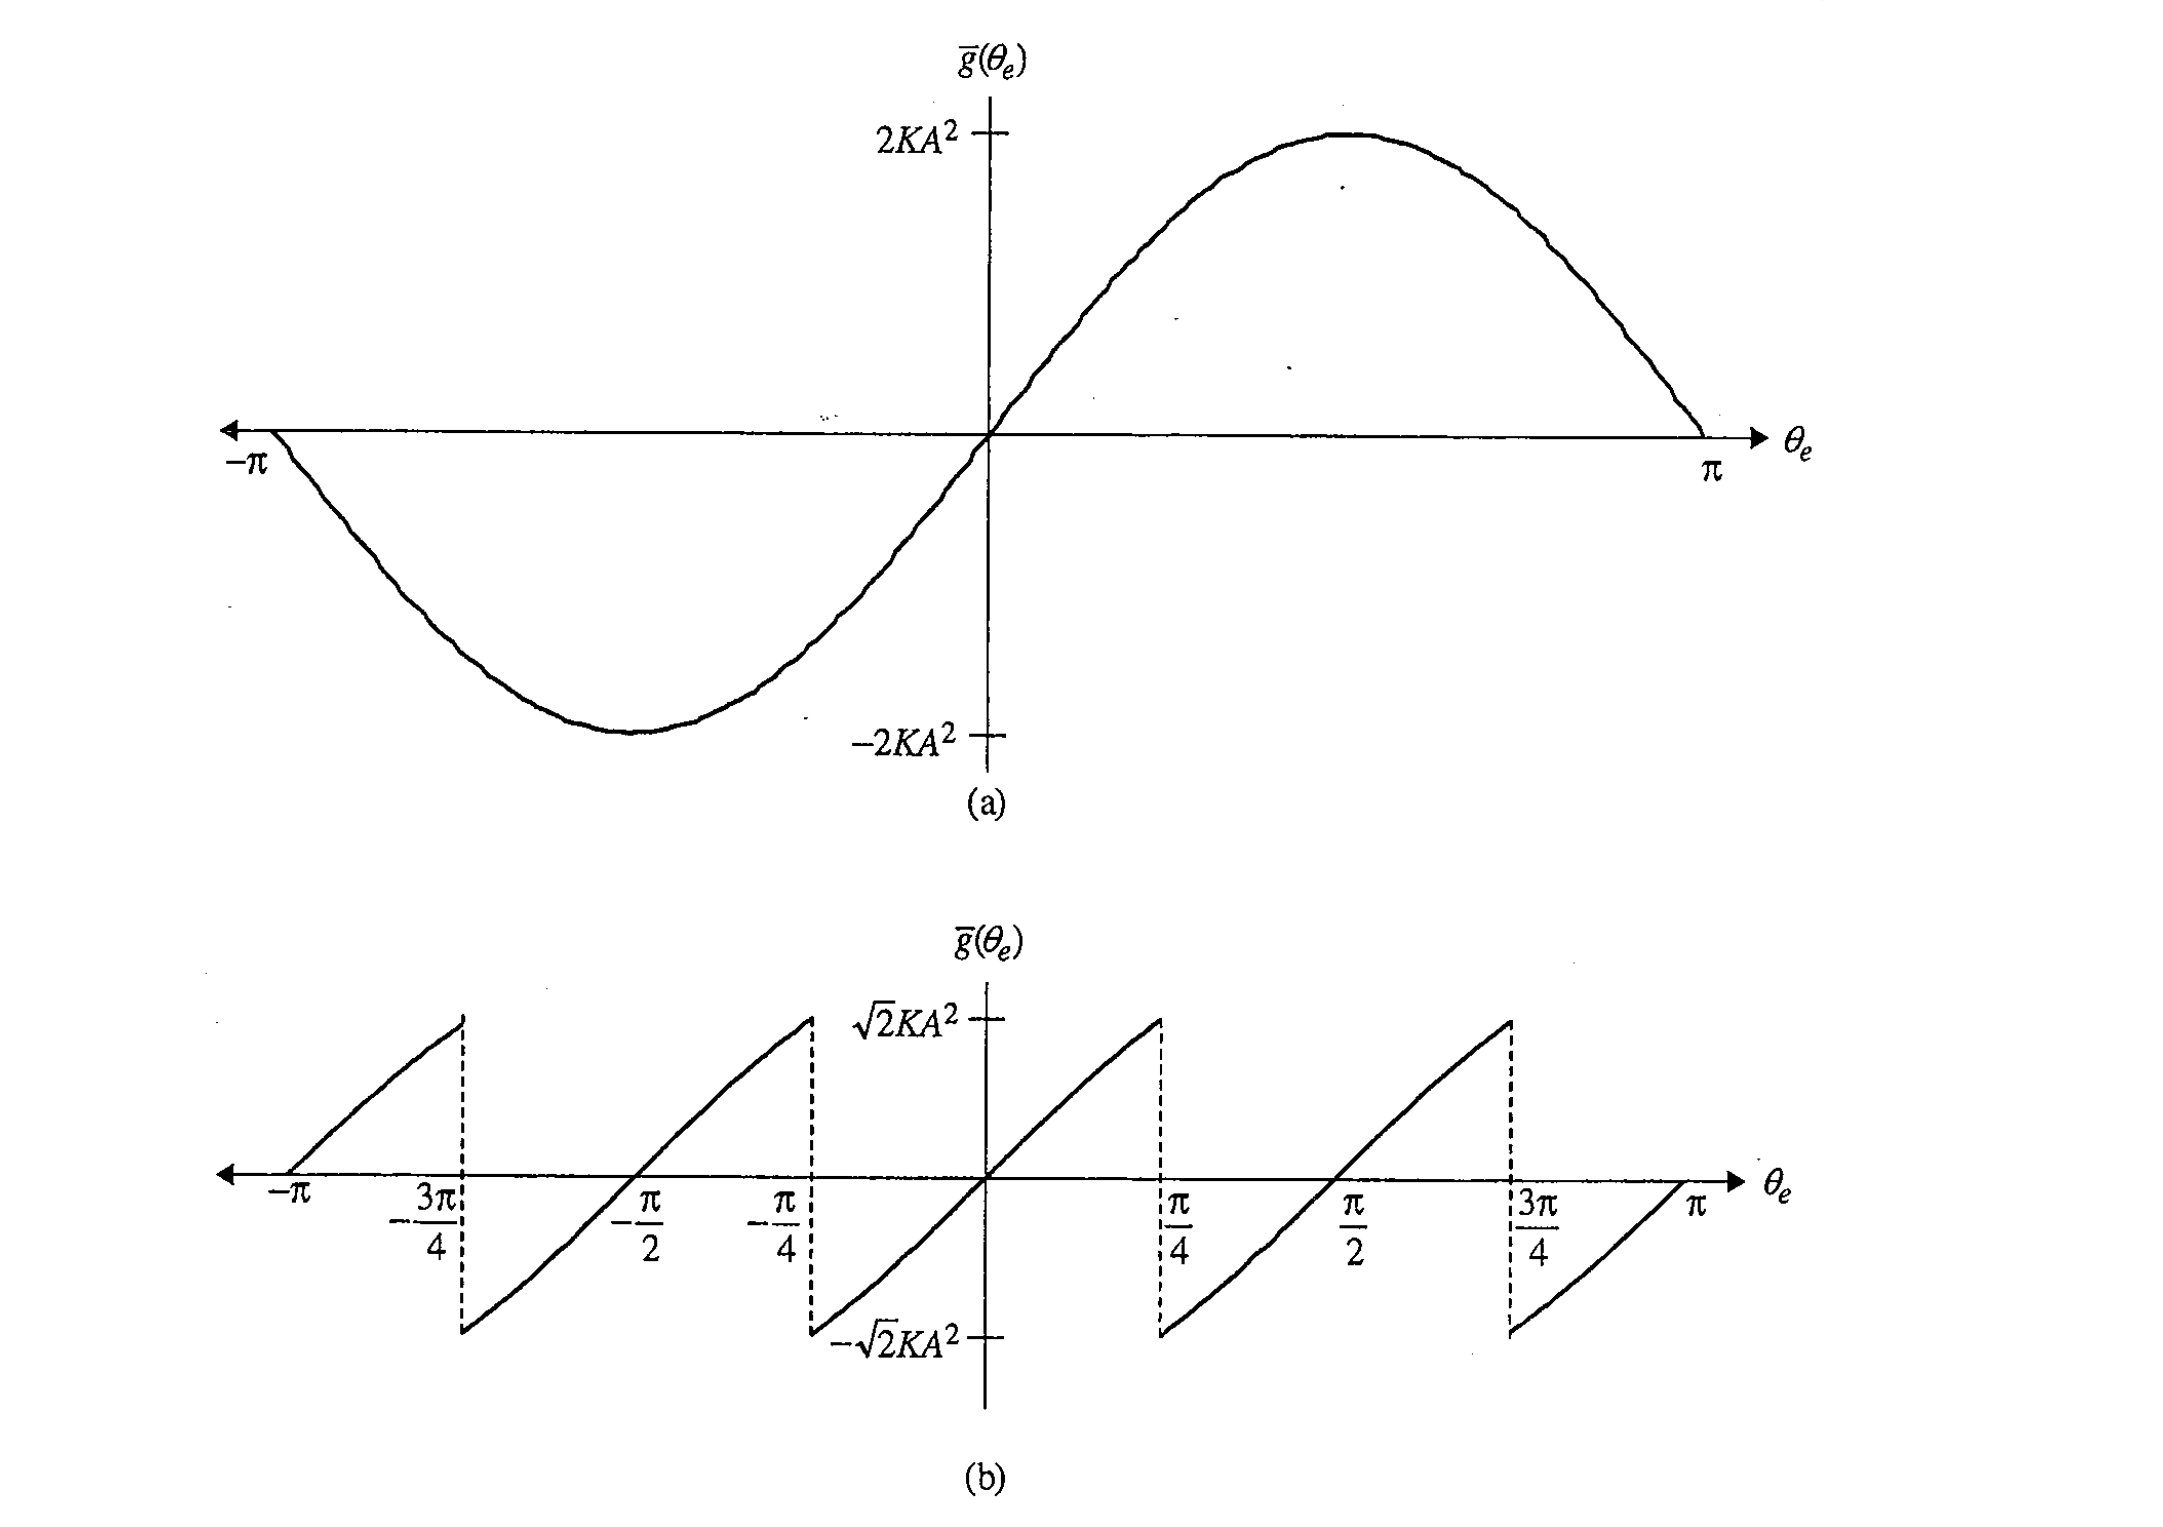
\includegraphics[width=\textwidth]{s_curve_qpsk}
  \caption{S-curves for the a) data-aided QPSK phase detector and b) the decision-directed QPSK phase detector [\citeauthor{digcomm_discrete_approach}]}
  \label{fig:s_curve_qpsk}
\end{figure}

\begin{figure}[ht]
  \centering
  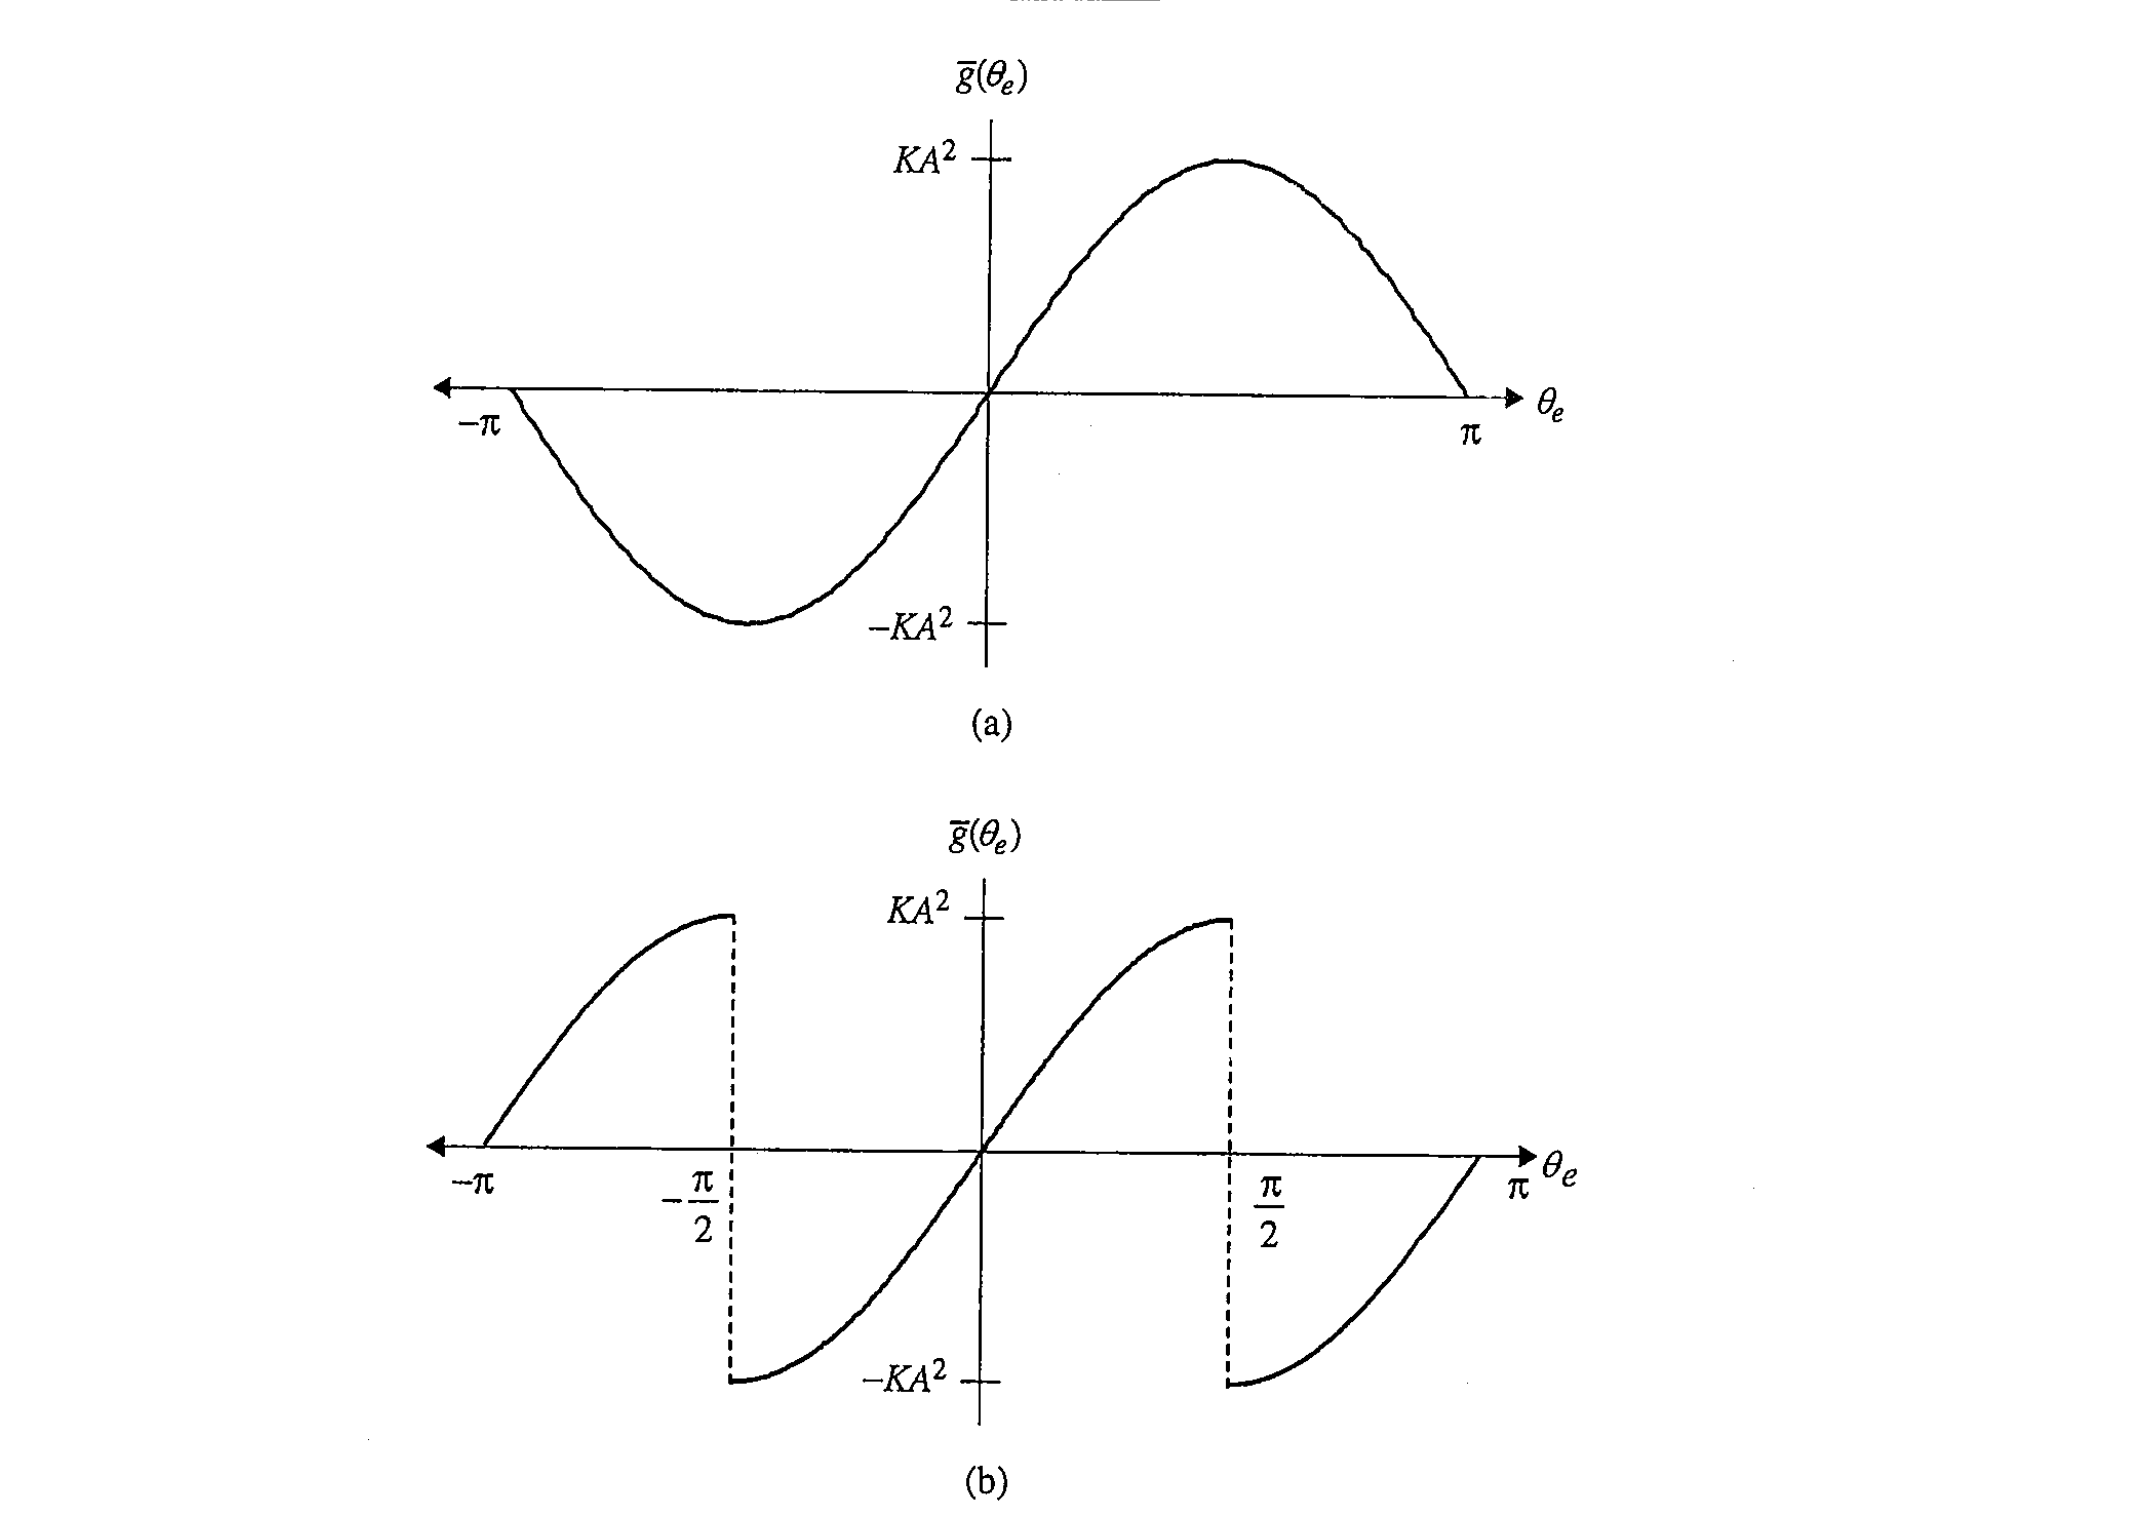
\includegraphics[width=\textwidth]{s_curve_bpsk}
  \caption{S-curves for the a) data-aided BPSK phase detector and b) the decision-directed BPSK phase detector [\citeauthor{digcomm_discrete_approach}]}
  \label{fig:s_curve_bpsk}
\end{figure}

Note the detector gain is dependent on the input sinal amplitude $K$ and so it's common to pass the input signal through a block such as an AGC, that adjusts the amplitude to the required value. Also note that the decision-directed QPSK case has 4 stable lock points (crosses zero with a positive slope), resulting in a $\frac{\pi}{2}$ phase ambiguity:
\begin{equation}
  \theta_e=-\frac{\pi}{2},0,\frac{\pi}{2},\pi
\end{equation}

Similarly, the BPSK case has 2 stable lock points ($\theta_e=0,\pi$), resulting in a $\pi$ phase ambiguity.

As for the remaining parameters, the damping factor $\zeta$ and the normalized loop bandwidth $B_nT$ are usually chosen by the designer to obtain the desired performance (a critically damped system is a popular choice). $K_0$, the DDS sensitivity, is usually taken to be 1. the remaining parameters $K_1$ and $K_2$ can be calculated given the two expressions previously given for the loop constants in \eqref{eq:digital_loop_constants1} and \eqref{eq:digital_loop_constants2}.

To conclude, an example of loop design with the ML detector is shown. Suppose the requirements specify QPSK modulation, an equivalent loop bandwidth of 2\% of the symbol rate ($B_n=0.02$) and a damping factor $\zeta=\frac{1}{\sqrt{2}}$. Assume for simplicity that $KA^2=1$ and also $K_0=1$. In this case, the proportional-plus-integrator loop filter constants are $K_1=2.6\times10^{-2}$ and $K_2=6.9\times10^{-4}$.

\autoref{fig:demo_fsync} show a Jupyter notebook example using the \code{FrequencySync} module to synchronize a QPSK signal embedded in AWGN noise and with an introduced phase and frequency offset.

\begin{figure}[ht]
  \centering
  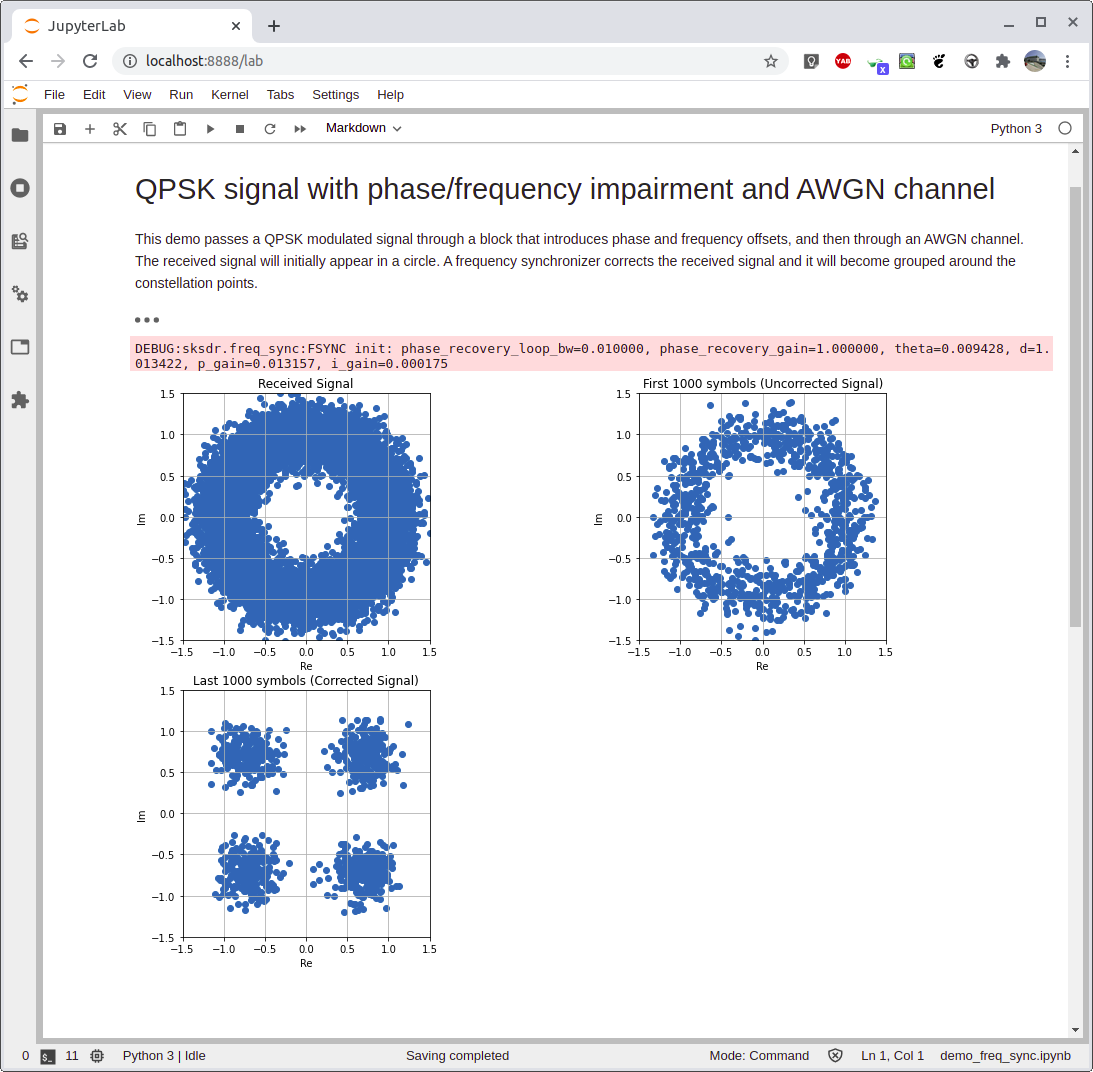
\includegraphics[width=0.75\textwidth]{demo_fsync}
  \caption{\code{FrequencySync} Jupyter notebook demonstration}
  \label{fig:demo_fsync}
\end{figure}

%%%%%%%%%%%%%%%%%%%%%%%%%%%%%%%%%%%%%%%%%%%%%%%%%%%%%%%%%%%%%%%%%%%%%%%%%%%%%%%
\section{Symbol Timing Synchronizer (PLL based)}

The \code{SymbolSync} module corrects symbol timing clock skew between a single-carrier transmitter and receiver. Currently it supports BPSK and QPSK modulation schemes.

\noindent Module properties:
\begin{itemize}
  \item \code{sps}: Samples per symbol of the input signal
  \item \code{mod}: Modulation of the input signal
  \item \code{damp\_factor}: PLL's damping factor
  \item \code{norm\_loop\_bw}: PLL's normalized loop bandwidth
  \item \code{K}: Input signal amplitude
  \item \code{A}: Symbol magnitude
\end{itemize}

Symbol timing synchronization consists of estimating a clock signal that is aligned in phase and frequency with the clock used to generate the data sequence at the transmitter. The clock is extracted from the (possibly noisy) received waveforms that carry the data and this estimate is used to identify the instants when the matched filter output should be sampled. \autoref{fig:drawing_sym2} shows the structure of the symbol timing synchronizer.

\begin{figure}[H]
  \centering
  \includegraphics[width=0.75\textwidth]{drawing_sym2}
  \caption{Discrete-time approach to symbol timing synchronization for sampled-data detectors}
  \label{fig:drawing_sym2}
\end{figure}

The algorithm is based on a discrete-time PLL algorithm, which consists of four components \cite{digcomm_discrete_approach}:
\begin{itemize}
  \item A timing error detector (TED)
  \item An interpolator
  \item An interpolation controller
  \item A loop filter
\end{itemize}

In terms of a discrete-time PLL structure, the interpolator and TED combination are the phase detector, and the interpolator control is the DDS. For more information, refer to \autoref{sect:library_freq_sync}, where an in-depth explanation of discrete-time PLL workings and parameters is presented.

Having a purely discrete-time architecture solves many of the problems associated with the continuous-time or hybrid approaches, such as phase noise on the voltage controlled clock (VCC) that drives the ADC. This however means that the ADC is not part of the loop and so the received signal $r(t)$ is sampled at a fixed rate $\frac{1}{T}$, that is asynchronous to the symbol rate $\frac{1}{T_s}$. As a consequence, this approach produces samples which are not aligned with the symbol boundaries. The role of the symbol timing synchronization is to `move' the samples to the desired time instants. Another name for `moving' samples in time is \emph{interpolation}. Because the synchronizer has to adapt to an unknown time delay, the interpolator needs to be adaptive. When working correctly, the interpolator produces matched filter outputs which are aligned with the symbols boundaries and the optimum sampling instant.

\subsection{Timing Error Detector}
\label{sect:timing_error_detector}

In general the detector produces an error signal once every symbol based on the current timing estimate $\hat \tau$ and the output of the matched filter $x(nT)$. The interpolator computes the interpolant $x(kT_s+\hat \tau)$ as:
\begin{equation}
x(kT_s+\hat\tau) = K\sum_{m} a(m)r_p\left(\left(k-m\right)T_s-\tau_e\right)
\end{equation}

where $\tau_e=\tau-\hat\tau$ is the timing error, $r_p$ is the autocorrelation function of the pulse shaping filter and $T_s$ is symbol period. The TED then produces a signal $g(\tau_e)$ that is a function of this timing error, in the same way the phase detector in a carrier frequency synchronizer produces a signal that is a function of the phase error. The characteristics of a TED, similarly to a phase error detector (PED), are described by its S-curve.

There are several TEDs in the literature and for this module the \emph{zero crossing TED} (ZCTED) has been chosen. It's a \emph{decision-directed} TED that offers similar performance to other alternatives, such as the \emph{maximum likelihood} TED (MLTED) and the \emph{early-late} TED (ELTED), but it is less susceptible to self-noise. This detector is based on finding the zero crossings in the eye diagram as opposed to the MLTED and ELTED which rely on the slope of the eye diagram. It operates at 2 samples/second and provides zero error when every other sample is time-aligned with a zero crossing in the matched filter output (the other samples are then time-aligned with the optimum sampling instants corresponding to maximum average eye opening). \autoref{fig:zero_crossing_detector} illustrates the operation of the ZCTED.

\begin{figure}[ht]
  \centering
  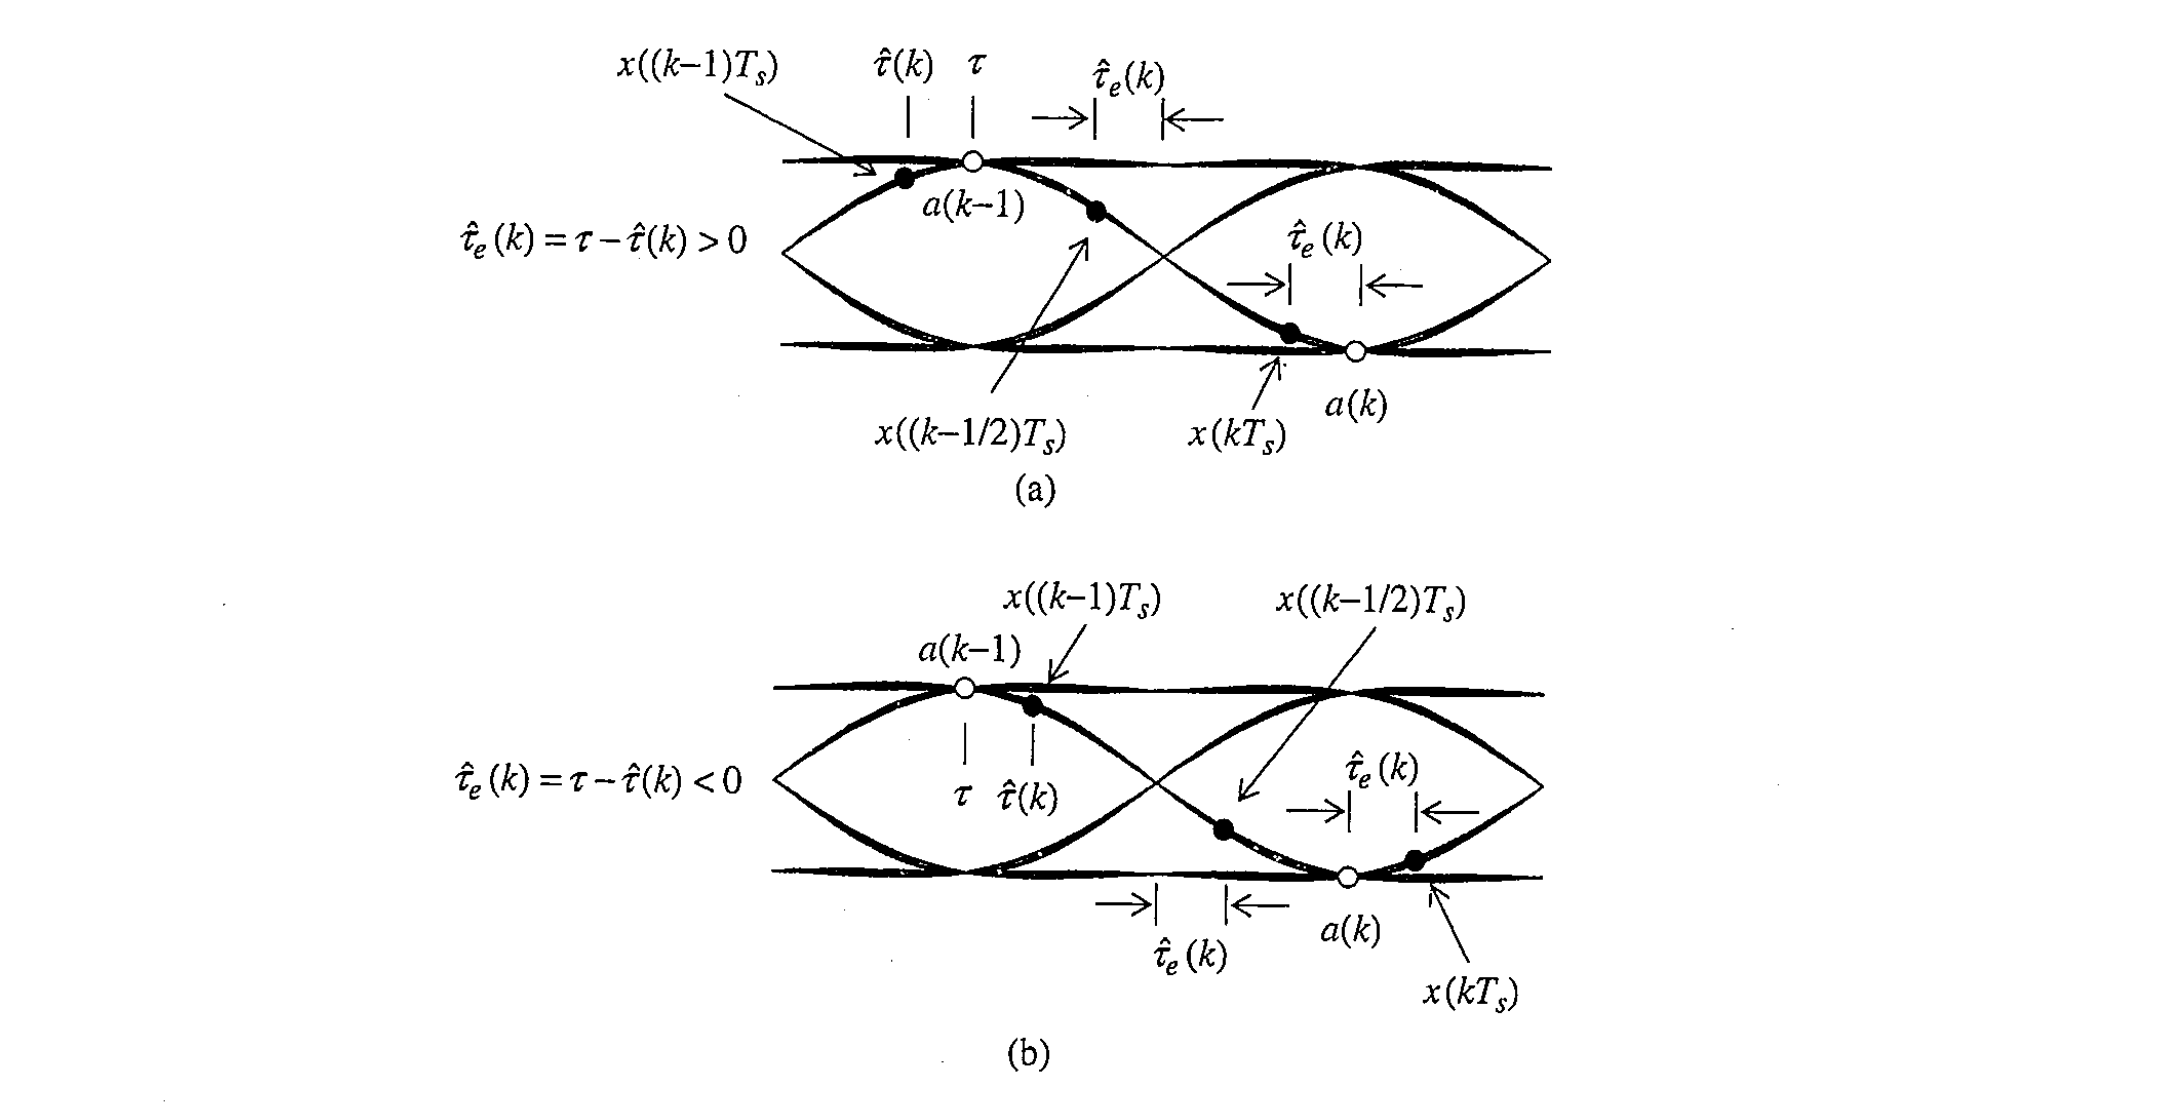
\includegraphics[width=\textwidth]{zero_crossing_detector}
  \caption{Operation of the zero-crossing TED. a) the timing estimate is early, b) the timing estimate is late [\citeauthor{digcomm_discrete_approach}]}.
  \label{fig:zero_crossing_detector}
\end{figure}

It can be shown \cite{digcomm_discrete_approach} that the error signal of the ZCTED is
\begin{equation}
e(k) = x\left(\left(k-1/2\right)T_s+\hat\tau\right)\left[\hat a\left(k-1\right)-\hat a\left(k\right)\right]
\end{equation}
where $\hat a(k)$ are the symbol estimates (for the decision-directed case), given by
\begin{align}
\hat a(k-1) &= A\times\operatorname{sgn}\left(x\left(\left(k-1\right)T_s + \hat\tau\right)\right)\\
\hat a(k)   &= A\times\operatorname{sgn}\left(x\left(\left(k\right)T_s + \hat\tau\right)\right)
\end{align}

An alternative is to use
\begin{align}
\hat a(k-1) &= \operatorname{sgn}\left(x\left(\left(k-1\right)T_s + \hat\tau\right)\right)\\
\hat a(k)   &= \operatorname{sgn}\left(x\left(\left(k\right)T_s + \hat\tau\right)\right)
\end{align}

This approximation provides the proper sign but not the proper amplitude for the estimation. This, however, does not appear to impact performance in any significant way.

The S-curve for the ZCTED can be obtained computing the expected value of $e(k)$ and assuming the symbols are uncorrelated. This can be shown to be
\begin{equation}
g(\tau_e)=K\cdot E_{avg}\left[ r_p\left(T_s/2-\tau_e\right) - r_p\left(-T_s/2-\tau_e\right) \right]
\end{equation}

The gain of the ZCTED, $K_p$, is the slope of $g(0)$ and is proportional to the received signal amplitude $K$ and the average symbol energy $E_{avg}$. This poses the same challenges as for the carrier frequency synchronization module, in the sense that $K$ must be either estimated and $K_p$ updated dynamically, or in alternative, $K$ must be kept within restricted values by use of an AGC block, for example. Finally because $r_p$ is a function of the pulse shaping filter, $K_p$ is also a function of the excess bandwidth, for the case of the root raised cosine filter.

\subsection{Interpolation}

The fundamental interpolation equation may be derived by considering a fictitious system involving continuous-time processing as illustrated in \autoref{fig:interpolation_dac}.

\begin{figure}[H]
  \centering
  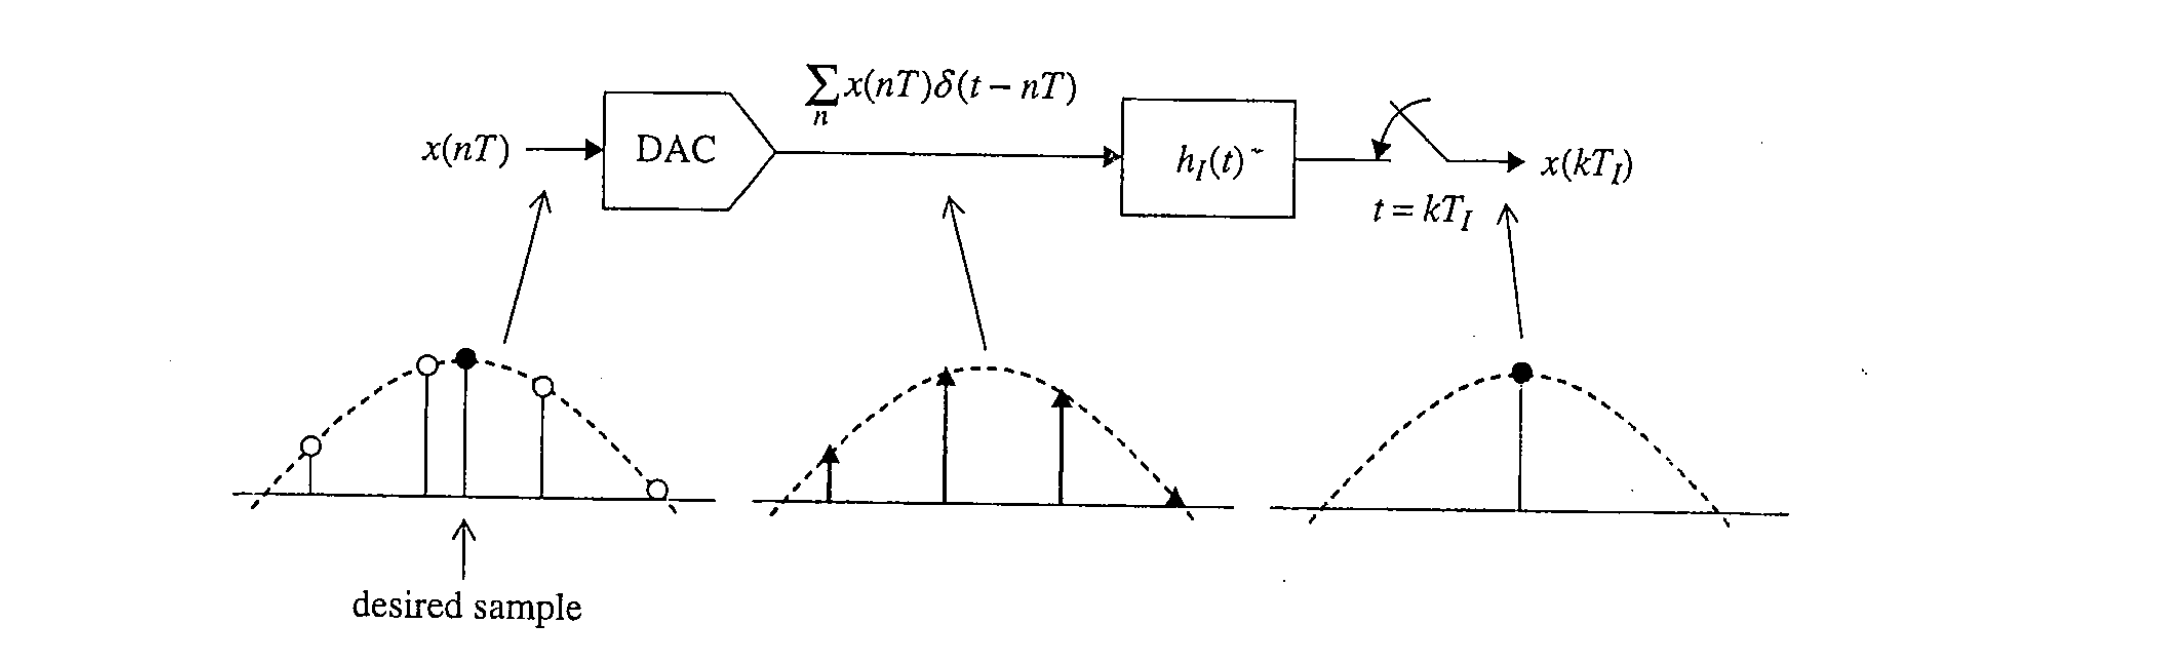
\includegraphics[width=\textwidth]{interpolation_dac}
  \caption{Ficticious system using continuous-time processing for performing interpolation [\citeauthor{digcomm_discrete_approach}]}
  \label{fig:interpolation_dac}
\end{figure}

First the input samples $x(nT)$ are converted to a weighted impulse train by the DAC. This impulse train is then filtered by an interpolation filter with impulse response $h_I(t)$ to produce the continuous time signal $x(t)$. Finally, to produce the desired samples, $x(t)$ is resampled at intervals $kT_I$ ($k=0,1,\ldots)$:
\begin{equation}
x(kT_I)=\sum_{n} x(nT)h_I(kT_I-nT)
\end{equation}

The desired sample, $x(kT_I)$, is called the $k$-th \emph{interpolant}. When the $k$-th interpolant is between samples $x(nT)$ and $x((n+1)T)$, the sample index $n$ is called the $k$-th \emph{basepoint index}, denoted by $m(k)$ and defined by $m(k)=\lfloor kT_I/T \rfloor$. The time instant $kT_I$ is some fraction of a sample time greater than $m(k)T$ and this fraction is called the $k$-th \emph{fractional interval}, denoted $\mu(k)$ and defined by $\mu(k)T=kT_I-m(k)T$. The previous expression for $x(kT_I)$ can be expressed in terms of these definitions using the filter index $i=m(k)-n$:
\begin{equation}
x(kT_I)=\sum_{i} x\left(\left(m(k\right)-i\right)T)h_I\left(\left(i+\mu\left(k\right)\right)T\right)
\end{equation}

\autoref{fig:interpolation} illustrates the principles behind the interpolation process.

\begin{figure}[H]
  \centering
  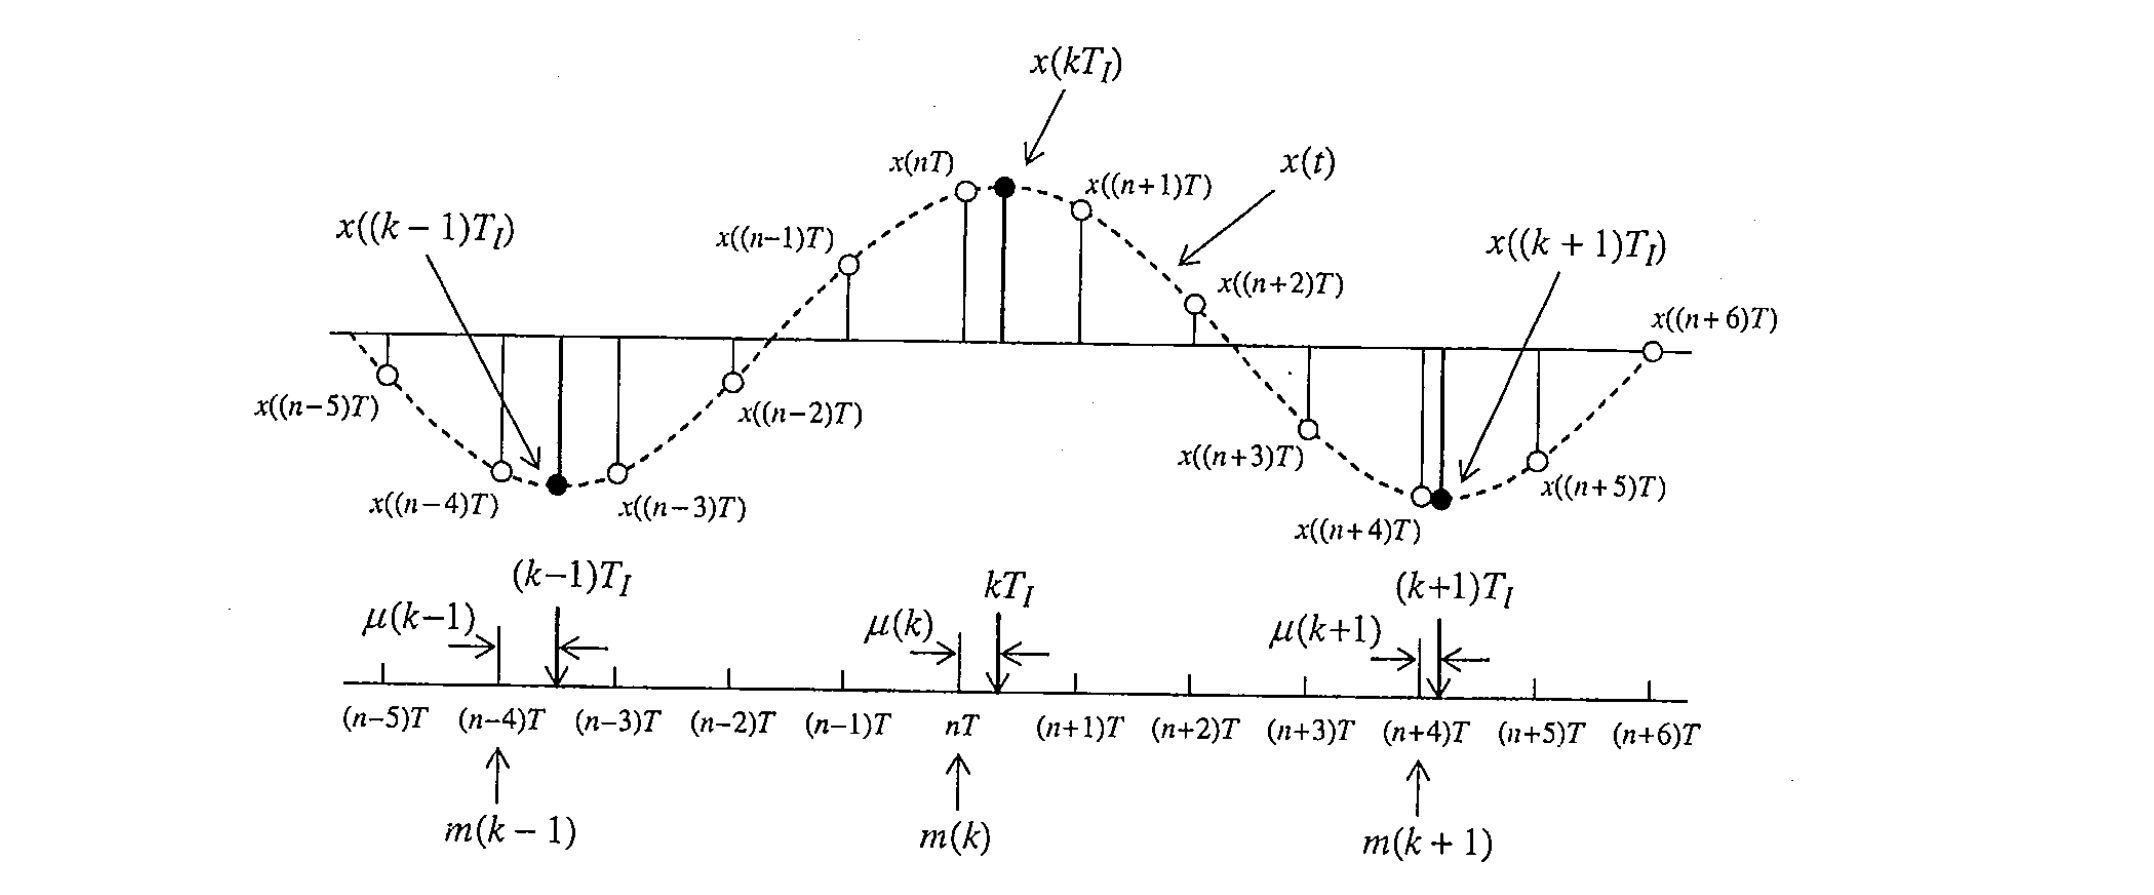
\includegraphics[width=\textwidth]{interpolation}
  \caption{Illustration of the relationships between the intepolation interval $T_I$, the sample time $T$, the basepoint indexes, and the fractional intervals [\citeauthor{digcomm_discrete_approach}]}
  \label{fig:interpolation}
\end{figure}

The optimum interpolation filter is an ideal low-pass filter with impulse response:
\begin{equation}
h_I(t)=\frac{\sin(\pi t/T)}{\pi t/T}
\end{equation}

Since this is unrealizable, one choice would be to massively upsample the matched filter input, match filter at the high sample rate and then downsample the output with the appropriately chosen sample offset. This is often denoted by a \emph{polyphase filterbank interpolator}. This technique is out of scope for this thesis and so will not be discussed. Another popular alternative is a class of FIR filters which approximate the ideal response, known as \emph{piecewise polynomial filters}. First, the underlying continuous waveform $x(t)$ is approximated by a polynomial in $t$:
\begin{equation}
x(t)\approx c_pt^p+c_{p-1}t^{p-1}+\ldots+c_1t+c_0
\end{equation}

Once the coefficients are known, the interpolant at $t=kT_I=\left(m(k)+\mu(k)\right)T$ is obtained by
\begin{equation}
x(kT_I)\approx c_p(kT_I)^p+c_{p-1}(kT_I)^{p-1}+\ldots+c_1(kT_I)+c_0
\end{equation}

When p = 1, this becomes
\begin{equation}
x((m(k)+\mu(k))T)=c_1((m(k)+\mu(k))T) + c_0
\end{equation}

The coefficients are determined by the available samples and satisfy
\begin{equation}\begin{bmatrix}
x(m(k)T)\\
x((m(k)+1)T)
\end{bmatrix}
=
\begin{bmatrix}
m(k)T & 1\\
(m(k)+1)T & 1
\end{bmatrix}
\begin{bmatrix}
c_1\\
c_0
\end{bmatrix}
\end{equation}

Solving for $c_0$ and $c_1$ gives
\begin{equation}
x((m(k)+\mu(k))T) = \mu(k)x((m(k)+1)T)+(1-\mu(k))x(m(k)T)
\end{equation}
which the linear interpolator.

There are four important observations:
\begin{enumerate}
  \item The interpolant is a linear combination of the available samples. As a consequence, it can thought of the output of an equivalent filter with coefficients
  \begin{equation}
  x((m(k)+\mu(k))T) = \sum_{i=-1}^{0}h_1(i)x((m(k)-i)T)
  \end{equation}
  where
  \begin{align}
  h_1(-1) &= \mu(k)\\
  h_1(0) &= 1 - \mu(k)
  \end{align}

  \item The equivalent filter coefficients are a function of the fractional interval $\mu(k)$ and not the base point $m(k)$. This is important to avoid overflow on the coefficients from the increasing base point index.

  \item The interpolating filter is a linear phase FIR filter, an important property. This can be seen because the coefficients are symmetric around the centre point of the filter $\mu(k) = 1/2$ and is a result of using an even number of samples to compute an interpolant that is between the middle two. It however poses a restrictions of using even number of coefficients and therefore an odd-degree polynomial.

  \item The sum of the coefficients is 1, and therefore independent of $\mu(k)$. This means the filter doesn't change the amplitude of the underlying waveform in the process of computing the interpolant.
\end{enumerate}

Having established the structure of piecewise polynomial approximation, a $p=2$ (second degree) polynomial is chosen, which is called a \emph{parabolic interpolator}. Given observation 3 though, it will have an additional parameter $\alpha$ to account for the extra degree of freedom introduced by having to use 4 points instead of 3. In the same way it was done for the linear interpolator, it can be shown that the coefficients of the equivalent filter in this case are

\begin{align}
h_3(-2) &= \alpha\mu(k)^2-\alpha\mu(k) \\
h_3(-1) &= -\alpha\mu(k)^2+(1+\alpha)\mu(k) \\
h_3(0) &= -\alpha\mu(k)^2-(1-\alpha)\mu(k)+1 \\
h_3(1) &= \alpha\mu(k)^2-\alpha\mu(k)
\end{align}

Using a piecewise polynomial interpolator to produce the interpolant will result in a computation of the form
\begin{equation}
x((m(k)+\mu(k))T)=\sum_{i=-I_1}^{I_2}h_p(i;\mu(k))x((m(k)-i)T)
\end{equation}
which is an approximation to the ideal filter response $h_I(t)$ defined earlier.

Because the coefficients $h_p$ are a function of $\mu(k)$, a hardware implementation requires 2-input multipliers with variable inputs. It can be shown that this can be optimized into a structure of the form
\begin{equation}
x((m(k)+\mu(k))T)=\sum_{l=0}^{p}\mu(k)^l\underbrace{\sum_{i=I_1}^{I_2} b_l(i)x((m(k)-i)T)}_{v(l)}
\end{equation}

In this form the inner sum becomes a filter equation in which the input data samples $x((m(k)-i)T)$ pass through a filter with impulse response $b_l(i)$. These coefficients are independent of $\mu(k)$. This can be further simplified by nested evaluation to the following structure, called a \emph{Farrow structure}\cite{farrow1988}, for a piecewise parabolic interpolator:
\begin{equation}
x((m(k)+\mu(k))T)=(v(2)\mu(k)+v(1))\mu(k)+v(0)
\end{equation}

The \emph{Farrow coefficients} for this interpolator are listed in \autoref{table:farrow_coeffs}.
\begin{table}[ht]
  \caption{Farrow coefficients for a piecewise parabolic interpolator}
  \label{table:farrow_coeffs}
  \centering
  \begin{adjustbox}{}
  \begin{tabular}{r | r | r | r}
  \toprule
  \thead{$i$} & \thead{$b_2(i)$} & \thead{$b_1(i)$} & \thead{$b_0(i)$} \\
  \hline
  $-2$ & $\alpha$ & $-\alpha$ & 0 \\
  $-1$ & $-\alpha$ & $1+\alpha$ & 0 \\
  $0$ & $-\alpha$ & $\alpha-1$ & 1 \\
  $1$ & $\alpha$ & $-\alpha$ & 0 \\
  \end{tabular}
  \end{adjustbox}
\end{table}

\subsection{Interpolator Control}

The function of interpolator control is to provide the interpolator with $k$-th basepoint $m(k)$ and the $k$-th fractional interval $\mu(k)$. One of the common methods for interpolator control, and used in this module, is the \emph{modulo-1 counter}. \autoref{fig:drawing_modulo_counter} shows its block diagram and \autoref{fig:modulo-1} illustrates the interpolation process from a time perspective.

\begin{figure}[H]
  \centering
  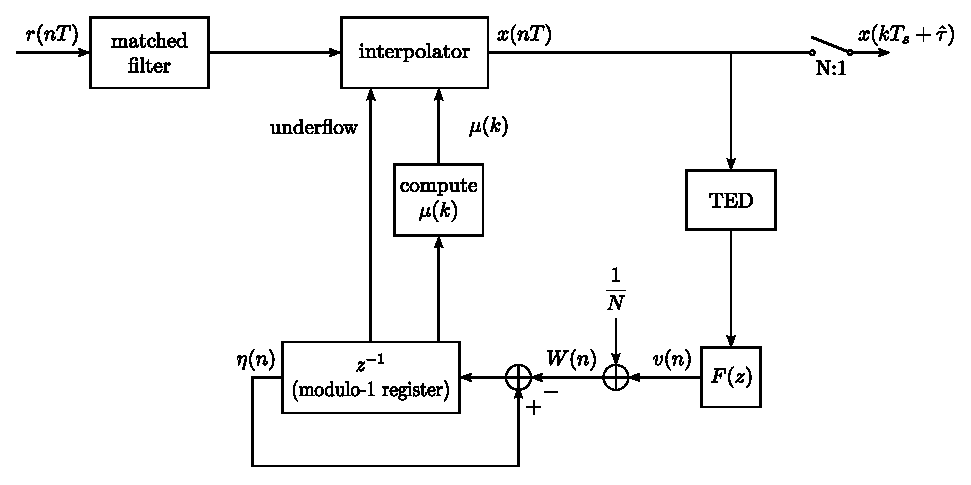
\includegraphics[width=\textwidth]{drawing_modulo_counter}
  \caption[Modulo-1 counter for interpolation control]{Modulo-1 counter for interpolation control. The basepoint index is identified by the underflow strobe and the fractional interval updated using the counter contents on underflow.}
  \label{fig:drawing_modulo_counter}
\end{figure}

\begin{figure}[H]
  \centering
  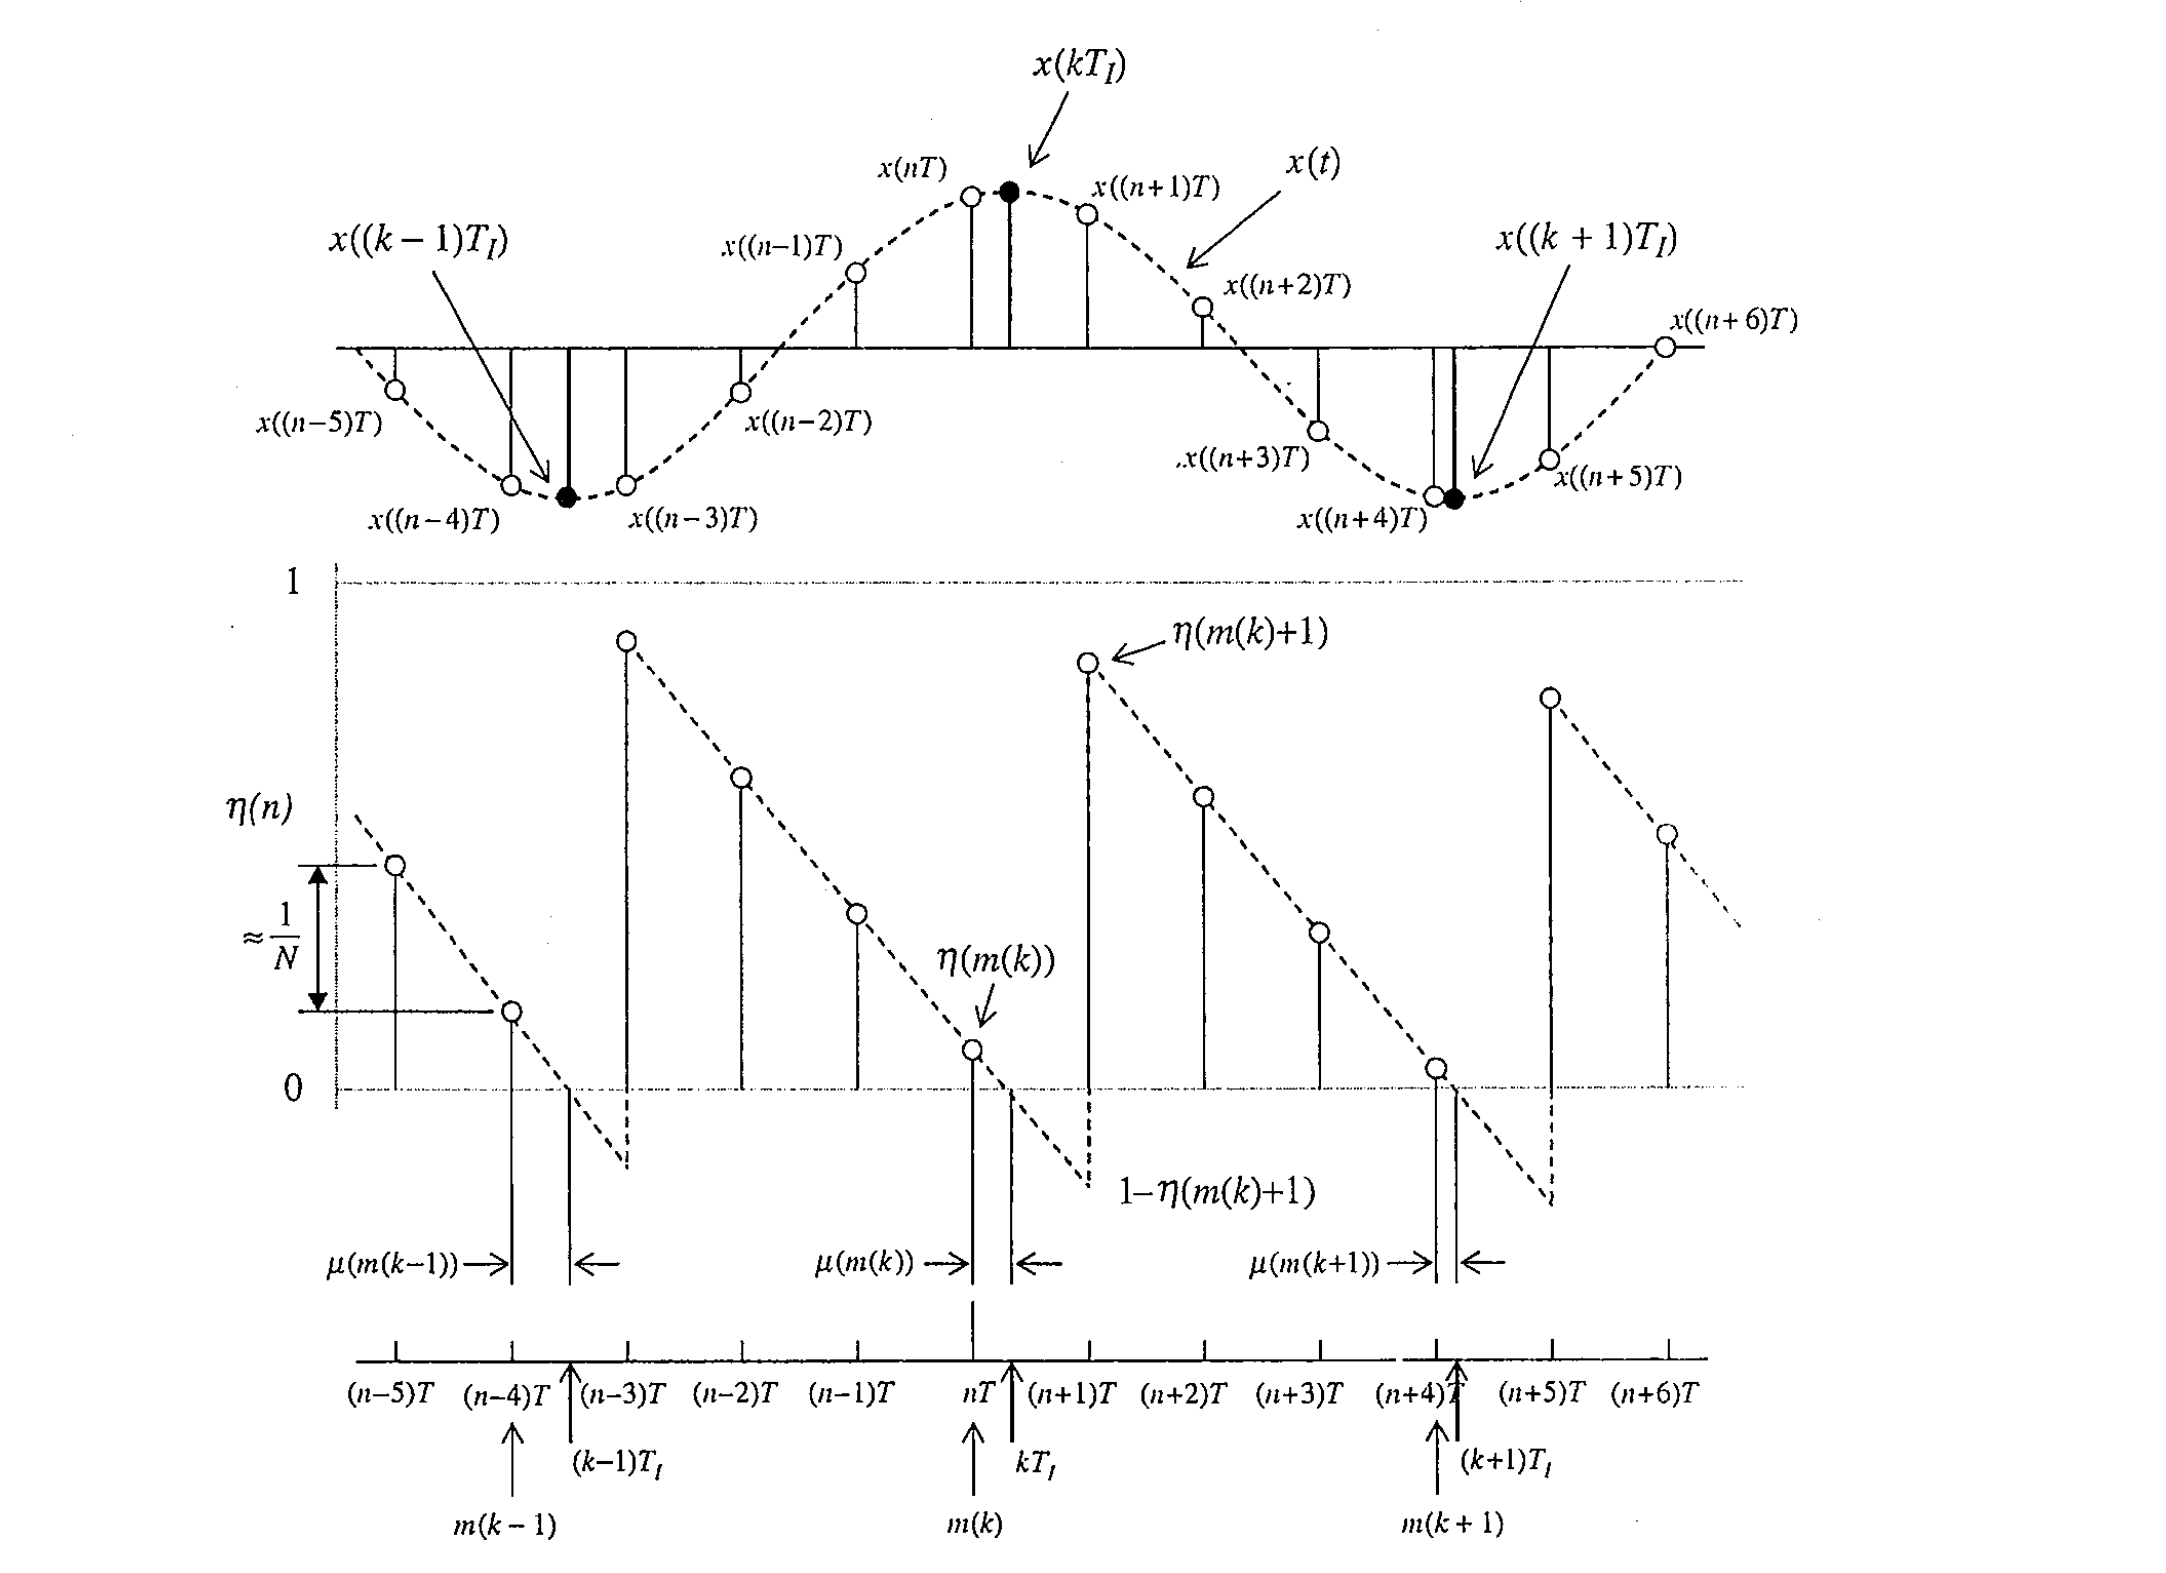
\includegraphics[width=\textwidth]{modulo-1}
  \caption{Illustration of the relationship between the available samples, the desired interpolants and the modulo-1 counter contents [\citeauthor{digcomm_discrete_approach}]}
  \label{fig:modulo-1}
\end{figure}

The counter decrements by $1/N$ so that the underflows occur every $N$ samples. The loop filter output $v(n)$ adjusts the amount by which the counter decrements. When operating correctly the underflow occurs 1 sample after the desired interpolant. The underflow condition is indicated by a \emph{strobe} and used by the interpolator to identify the basepoint index. The fractional interval is obtained from the contents of the modulo-1 counter on underflow. In general, the counter values satisfies the recursion
\begin{equation}
\eta(n+1)=\left(\eta(n)-W(n)\right)\operatorname{mod}1
\end{equation}
where $W(n)=1/N+v(n)$. When the decrementing counter underflows, the index $n$ is the basepoint index $m(k)$. Incorporating the modulo-1 reduction produces
\begin{equation}
  \eta\left(m(k)+1\right)=1+\eta\left(m(k)\right)-W\left(m(k)\right)
\end{equation}

As illustrated in \autoref{fig:modulo-1}, the counter values $\eta(m(k))$ and $1-\eta(m(k)+1)$ for similar triangles. This observation leads to the relationship
\begin{equation}
\frac{\mu(m(k))}{\eta(m(k))}=\frac{1-\mu(m(k))}{1-\eta((m(k)+1))}
\end{equation}

Solving for $\mu(m(k))$ gives
\begin{equation}
\mu(m(k))=\frac{\eta(m(k))}{W(m(k))}
\end{equation}

The underflow period (in samples) is
\begin{equation}
\frac{1}{W(n)}=\frac{N}{1+Nv(n)}
\end{equation}

When in lock, $v(n)$ is zero on average, and the decrementing modulo-1 counter underflow period is $N$ samples on average. During acquisition, $v(n)$ aligns the underflow periods to align the symbol boundaries. The decrementing modulo-1 counter plays the same role in this system as the DDS plays in a phase/frequency synchronization PLL and its modulo-1 operation corresponds to the modulo-$2\pi$ operation of the DDS. Noting that the gain $K_0$ is $-1$ in this case, instead of $1$, because it's a decrementing counter.

\autoref{fig:demo_symbol_sync} show a Jupyter notebook example using this module to synchronize a QPSK signal embedded in AWGN noise and with an introduced timing delay.

\begin{figure}[H]
  \centering
  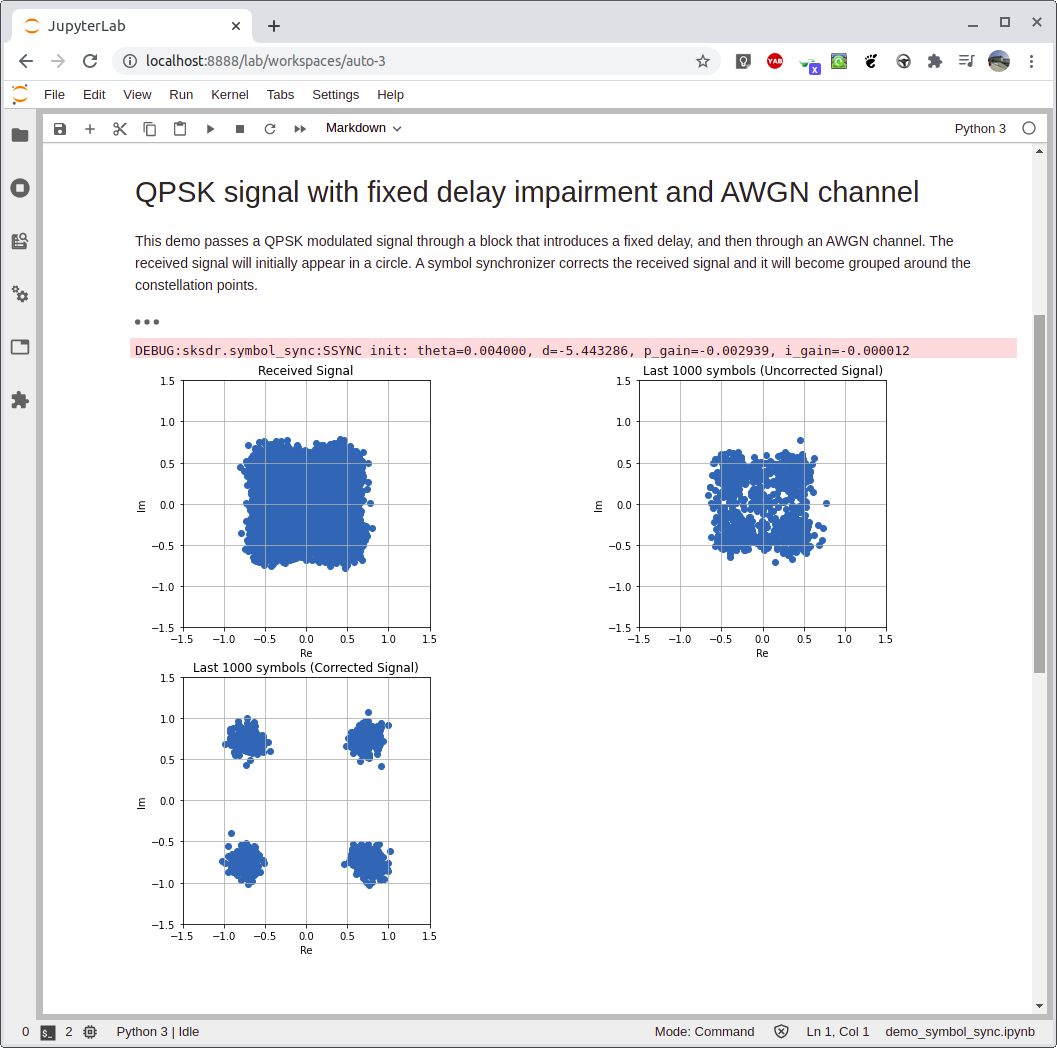
\includegraphics[width=0.75\textwidth]{demo_symbol_sync}
  \caption{\code{SymbolSync} Jupyter notebook demonstration}
  \label{fig:demo_symbol_sync}
\end{figure}

%%%%%%%%%%%%%%%%%%%%%%%%%%%%%%%%%%%%%%%%%%%%%%%%%%%%%%%%%%%%%%%%%%%%%%%%%%%%%%%
\section{Automatic Gain Control}

The AGC module adaptively adjusts its gain to achieve a constant output power.

\noindent Module properties:
\begin{itemize}
  \item \code{ref\_power}: Desired output power
  \item \code{max\_gain} (dB): Upper limit on the loop gain
  \item \code{det\_gain}: Detector gain
  \item \code{avg\_len} (samples): Length of moving average filter
\end{itemize}

The module doesn't use a linear loop scheme since that has a significant drawback: The time constant of the loop is input signal level dependent, and is different depending on whether the input signal is increasing or decreasing. These properties drastically reduce the control over the system's time constant. To solve this problem, a logarithmic loop is adopted. This allows control of the AGC's time constant, increases its dynamic range and generally provides good performance for a variety of signal types. \autoref{fig:agc_diagram} shows a block diagram of the algorithm.

% \begin{figure}[ht]
% \centering
% \begin{tikzpicture} [circuit ee IEC,
%                       small circuit symbols,
%                       every info/.style={font=\footnotesize},
%                       set make contact graphic= var make contact IEC graphic,
%                       skip loop/.style={to path={-- ++(0,-1) -| (\tikztotarget)}},
%                       skip loop left/.style={to path={-- ++(-1,0) |- (\tikztotarget)}}]

% \matrix (m1) [row sep=10mm, column sep=10mm]
% {
%   %--------------------------------------------------------------------
%   \node[dspnodeopen,dsp/label=above] (m00) {$x(n)$}; &
%   \node[dspmixer] (m01) {}; &
%   \node[coordinate] (m02) {1}; &
%   \node[coordinate] (m03) {2}; &
%   \node[coordinate] (m04) {}; &
%   \node[coordinate] (m05) {}; &
%   \node[coordinate] (m06) {}; &
%   \node[coordinate] (m07) {}; &
%   \node[dspnodefull] (m08) {}; &
%   \node[dspnodeopen,dsp/label=above] (m09) {$y(n)$}; \\
%   %--------------------------------------------------------------------
%   \node[coordinate] (m10) {}; &
%   \node[dspsquare] (m11) {$\exp$}; &
%   \node[coordinate] (m12) {}; &
%   \node[coordinate] (m13) {}; &
%   \node[dspnodeopen,dsp/label=above] (m14) {$K$}; &
%   \node[dspnodeopen,dsp/label=above] (m15) {$\ln(A)$}; &
%   \node[coordinate] (m16) {}; &
%   \node[coordinate] (m17) {}; &
%   \node[dspmixer] (m18) {}; &
%   \node[coordinate] (m19) {}; \\
%   %--------------------------------------------------------------------
%   \node[coordinate] (m20) {}; &
%   \node[dspnodefull] (m21) {}; &
%   \node[dspsquare] (m22) {$z^{-1}$}; &
%   \node[dspadder] (m23) {}; &
%   \node[dspmixer] (m24) {}; &
%   \node[dspadder] (m25) {}; &
%   \node[dspsquare] (m26) {$\ln$}; &
%   \node[dspsquare,inner xsep=1mm] (m27) {LPF}; &
%   \node[coordinate](m28) {}; \\
% };

% \begin{scope}[start chain]
%   \chainin (m00);
%   \chainin (m01) [join=by dspconn];
%   \chainin (m08) [join=by dspflow];
%   \chainin (m09) [join=by dspconn];
% \end{scope}

% \begin{scope}[start chain]
%   \chainin (m08) [join=by dspconn];
%   \chainin (m18) [join=by dspconn];
%   \chainin (m28) [join=by dspline];
%   \chainin (m27) [join=by dspconn];
%   \chainin (m26) [join=by dspconn];
%   \chainin (m25) [join=by dspconn];
%   \chainin (m24) [join=by dspconn];
%   \chainin (m23) [join=by dspconn];
%   \chainin (m22) [join=by dspconn];
%   \chainin (m21) [join=by dspline];
%   \chainin (m11) [join=by dspconn];
%   \chainin (m01) [join=by dspconn];
% \end{scope}

% \draw[dspconn] (m14) to (m24);
% \draw[dspconn] (m15) to (m25);
% \path (m21.south)
%   edge[dspconn,skip loop] (m23.south);
% \path ($ (m08) + (0,-2mm) $)
%   edge[dspconn,skip loop left] (m18.west);
% \draw[dspline] (m26) -- node[near end,below] {$-$} (m25);

% \end{tikzpicture}
% \caption{AGC diagram}
% \label{fig:agc_diagram}
% \end{figure}

\begin{figure}[H]
  \centering
  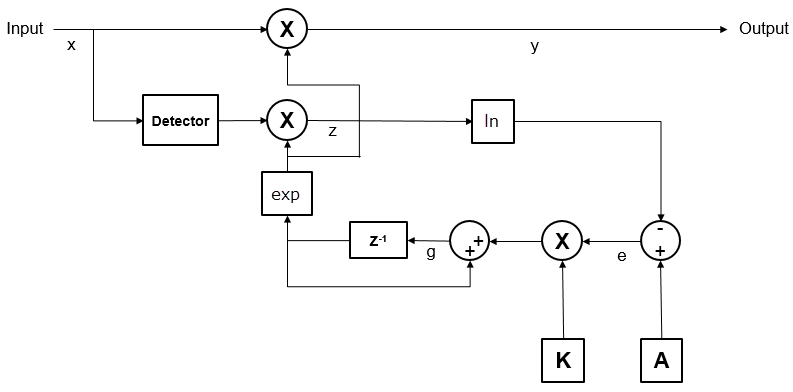
\includegraphics[width=0.80\textwidth]{agc_diagram}
  \caption{AGC block diagram [\citeauthor{mathworks_agc}]}
  \label{fig:agc_diagram}
\end{figure}

The detector block is composed of a low-pass filter (LPF) to eliminate rapid gain changes. That filter can be a simple moving average filter, a cascaded integrator-comb (CIC) filter, or a more traditional low-pass filter having a sinc-shaped impulse response. In the current implementation, a moving average filter is implemented, which computes the average power of the last \code{avg\_len} samples. This power is then multiplied by the loop gain $g(n)$ and compared with the reference power $A$ (specified by \code{ref\_power}) in natural log units, to produce the error signal $e(n)$. This error signal is scaled by the detector gain $K$(specified by \code{det\_gain}) and passed to an integrator which updates the loop gain $g(n)$.

Mathematically, the algorithm is summarized as:
\begin{align}
y(n) & = x(n)\cdot e^{g(n-1)}\\
z(n) & = D(x(n))\cdot e^{2g(n-1)}\\
e(n) & = \ln(A)-\ln(z(n))\\
g(n) & = g(n-1)+K\cdot e(n)\\
\end{align}
where
\begin{itemize}
  \item $x(n)$ is the input signal,
  \item $y(n)$ is the output signal,
  \item $g(n)$ is the loop gain, in Neper
  \item $D()$ is the detector function,
  \item $z(n)$ is the detector output,
  \item $e(n)$ is the error signal,
  \item $A$ is the reference value, given by \code{ref\_power},
  \item $K$ is the detector gain, given by \code{det\_gain}
\end{itemize}

The detector function $D(\ldots)$, as mentioned, is implemented as a moving average filter:
\begin{equation}D(n)=\frac{1}{N}\sum_{m=0}^{N-1}|x(n-m)|^2\end{equation}
where $N$ is the number of samples to average, given by \code{avg\_len}.

\autoref{fig:demo_agc_interface} shows the Jupyter interface developed for this demonstration. \autoref{fig:demo_agc} shows the results where it is visible that the output signal power converges to the specified value, while the error signal converges to zero.

\begin{figure}[H]
  \centering
  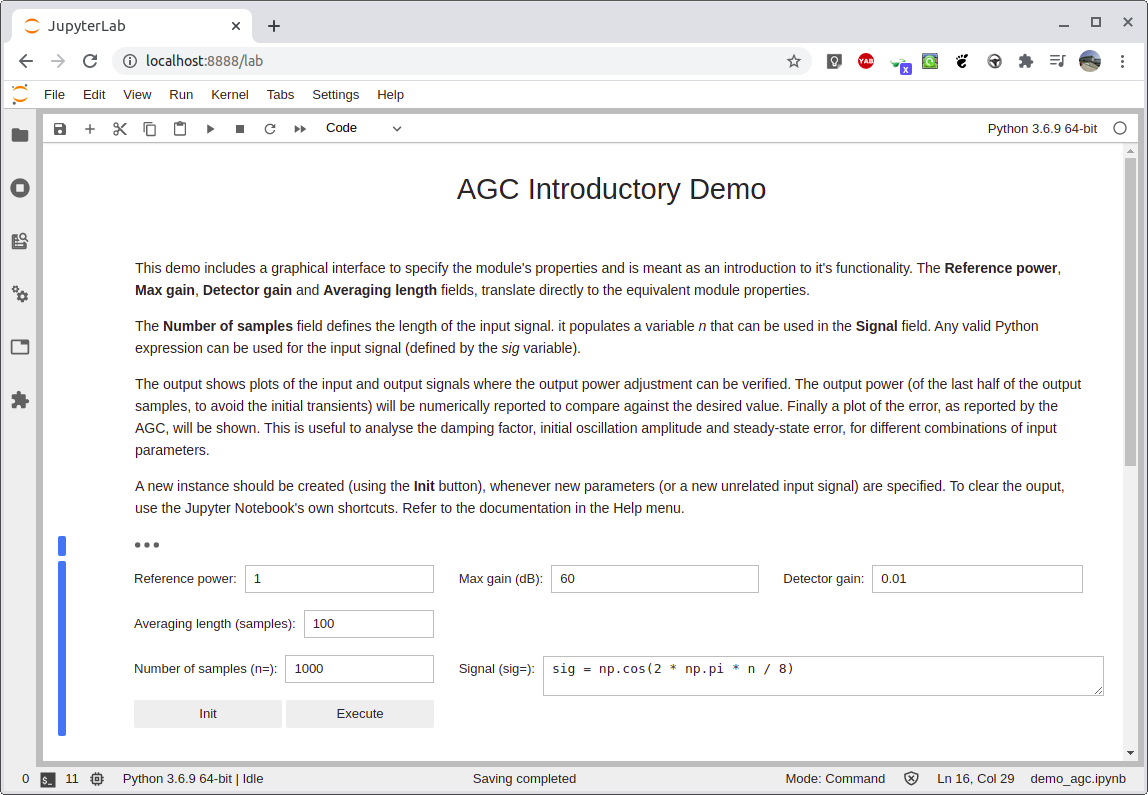
\includegraphics[width=0.75\textwidth]{demo_agc_interface}
  \caption{\code{AGC} Jupyter notebook demonstration interface}
  \label{fig:demo_agc_interface}
\end{figure}

\begin{figure}[H]
  \centering
  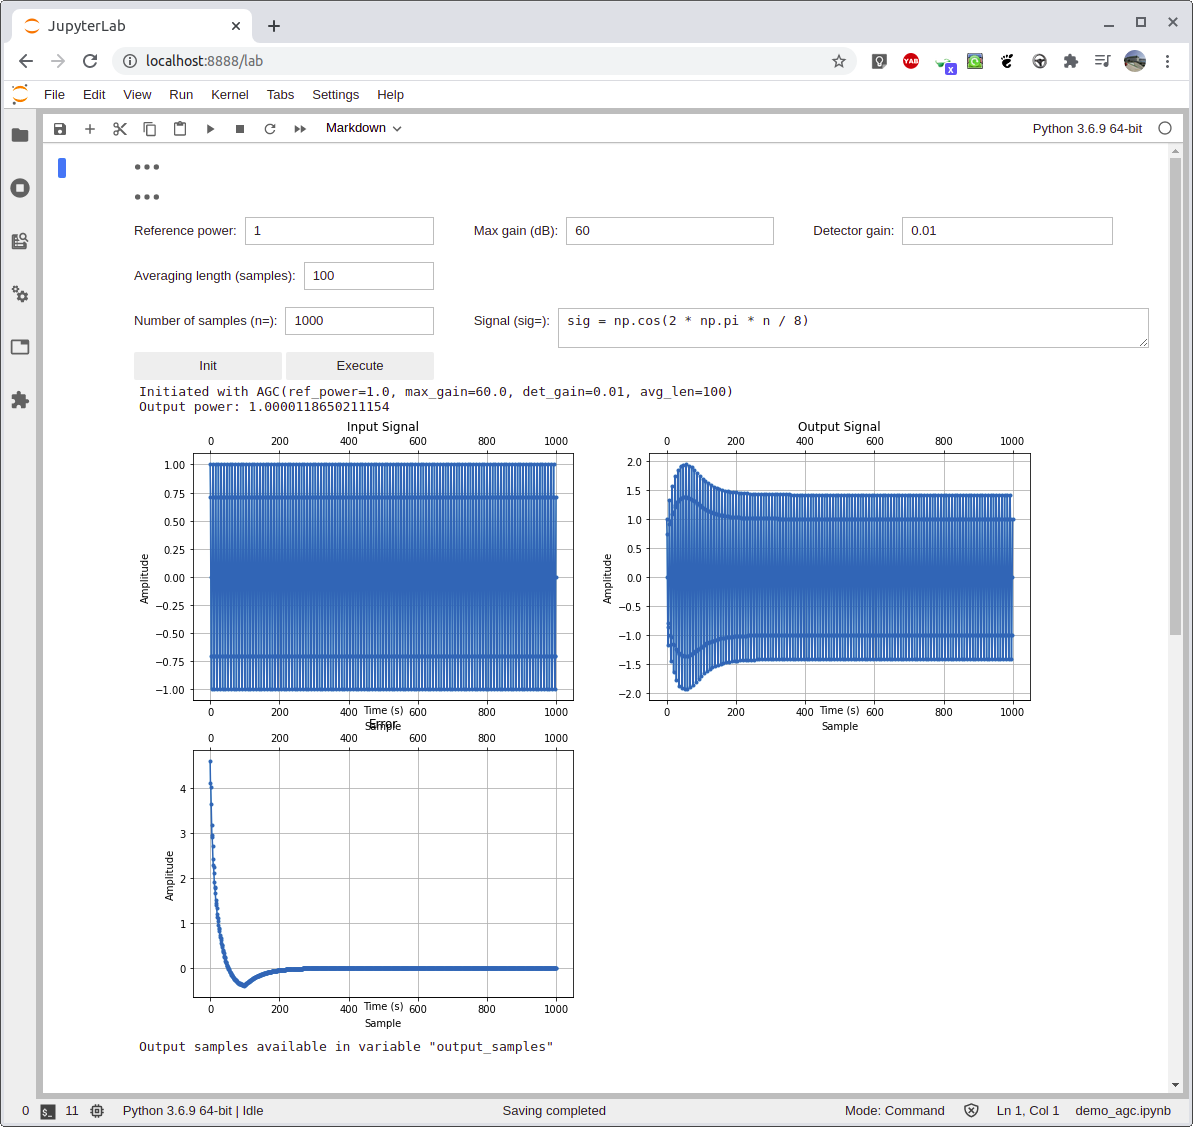
\includegraphics[width=0.75\textwidth]{demo_agc}
  \caption{\code{AGC} Jupyter notebook demonstration results}
  \label{fig:demo_agc}
\end{figure}

%%%%%%%%%%%%%%%%%%%%%%%%%%%%%%%%%%%%%%%%%%%%%%%%%%%%%%%%%%%%%%%%%%%%%%%%%%%%%%%
\section{Phase Ambiguity Correction}

As mentioned in \autoref{sect:library_freq_sync} and seen in the S-curves from \autoref{fig:s_curve_qpsk} and \autoref{fig:s_curve_bpsk}, the phase detector algorithm can lock onto a phase that $\pm 180\degree$ from the correct phase (for BPSK) and $[\pm 90\degree,\pm 180\degree,\pm 270\degree]$ for QPSK. This module resolves this ambiguity.

\noindent Module properties:
\begin{itemize}
  \item \code{preamble}: The modulated preamble, as sent by the transmitter
\end{itemize}

The module takes a known sequence, like a preamble, and compares the phase of this sequence with the phase of the same sequence embedded in the input signal (which could have an erroneous phase offset). The algorithm can be described as follows:
\begin{itemize}
  \item The input signal is expressed as $x(n) = p(n)e^{j\phi} + w(n)$, where $p(n)$ is the preamble, $\phi$ is the phase to be estimated and $w(n)$ is a noise term.
  \item Compute $y_1(t) = p^*(n)x(n) = e^{j\phi} + x^*(n)w(n)$, where $*$ denotes complex conjugation.
  \item The goal is to estimate the value $\phi$ from the observation $y_1(n)$, i.e., estimate the value $B = e^{j\phi}$, and $\phi = \text{angle}(B)$. Suppose $w(n)$ yields a i.i.d. complex AWGN distribution $\mathcal{N}(0,\sigma^2)$. Then a non-biased estimator could be $\hat{B} = \frac{1}{N}\sum_{n=0}^{N-1} y_1(n)$, where $N$ is the number of samples in the preamble. In that case $\hat\phi = \text{angle}(\hat{B})$ and the variance of the estimator $\hat{B}$ is $\frac{\sigma^2}{N}$.
  \item Once $\phi$ has been estimated, remove it from the input signal. The output signal becomes $y(n) = x(n)e^{-j\phi}$.
\end{itemize}

%%%%%%%%%%%%%%%%%%%%%%%%%%%%%%%%%%%%%%%%%%%%%%%%%%%%%%%%%%%%%%%%%%%%%%%%%%%%%%%
\section{Channel Models and Impairments}
This sections describes the channel models and impairments available in the SKSDR library.

\subsection{AWGN Channel}

The \code{AWGNChannel} class implements a simple \emph{additive white Gaussian channel noise} model.

\noindent Module properties:
\begin{itemize}
  \item \code{snr}: The desired SNR
  \item \code{signal\_power}: The expected signal power, or `measured' if the power is to measured dynamically each time the module is invoked.
\end{itemize}

The algorithm draws the noise as values from the standard normal distribution, scaled to the appropriate power in order to fulfil the desired SNR (specified by the \code{snr} property). It then returns the input signal added to this generated noise.

\subsection{Phase/Frequency Impairment}
The \code{PhaseFrequencyOffset} module applies phase and frequency offsets to an incoming signal.

\noindent Module properties:
\begin{itemize}
  \item \code{sample\_rate} (Hz): The input signal sample rate
  \item \code{freq\_offset} (Hz): The desired frequency offset
  \item \code{phase\_offset} (degrees): The desired phase offset
\end{itemize}

The phase offset parameter (specified by \code{phase\_offset}) adds a constant to the phase of the signal. The frequency offset parameter (specified by \code{freq\_offset}) determines the rate of change of the signal's phase. If one sets the frequency offset to a positive number, the symbol points on a scatter plot, will fall on a rotating grid, corresponding to the standard constellation, which revolves at a constant rate in the counter-clockwise direction.

Given an input sequence $x(n)$, the module computes
\begin{align}
  y(n) = x(n)e^{j(\omega nT + \phi)}
\end{align}
where $\omega$ is the frequency offset, $T$ is the sampling period and $\phi$ is the phase offset.

\autoref{lst:demo_phase_freq_offset} shows a demo of this module, using IPython. A phase offset of 30° and a frequency offset of 1\% of the sample rate are introduced in a QPSK signal. The original signal and signals with offsets are plotted for comparison. \autoref{fig:demo_phase_freq_offset} shows the resulting scatter plots.

\begin{python}[label={lst:demo_phase_freq_offset},caption={\code{PhaseFrequencyOffset} demo}]
  In [1]: import matplotlib.gridspec as gridspec
  ...: import matplotlib.pyplot as plt
  ...: import numpy as np
  ...:
  ...: import sksdr
  ...:
  ...: # Create a phase and frequency offset object, where the phase offset is 30 degrees
  ...: pfo_phase = sksdr.PhaseFrequencyOffset(phase_offset=30, sample_rate=1e6)
  ...:
  ...: # Create a phase and frequency offset object, where the frequency offset is
  ...: # 1 percent of the sample rate
  ...: pfo_freq = sksdr.PhaseFrequencyOffset(freq_offset=1e4, sample_rate=1e6)
  ...:
  ...: # Generate random data symbols and apply QPSK modulation
  ...: ints = np.random.randint(0, 4, 1000)
  ...: bits = sksdr.x2binlist(ints, 2)
  ...: psk = sksdr.PSKModulator(sksdr.QPSK, [0, 1, 3, 2], 1.0, np.pi/4)
  ...: mod_sig = psk.modulate(bits)
  ...:
  ...: # Apply phase and frequency offsets
  ...: mod_sig_phase_off, _ = pfo_phase(mod_sig)
  ...: mod_sig_freq_off, _ = pfo_freq(mod_sig)
  ...:
  ...: # Setup figure
  ...: fig = plt.figure(figsize=(15,10))
  ...: gs = gridspec.GridSpec(2, 2, figure=fig)
  ...:
  ...: # Scatter plot of the original signal
  ...: f = sksdr.scatter_plot(mod_sig, 'Original Signal', fig=fig, gs=gs[0, 0])
  ...:
  ...: # Scatter plot of the signal with phase offset
  ...: f = sksdr.scatter_plot(mod_sig_phase_off,
  ...:                        'Signal with phase offset of 30 degrees',
  ...:                        fig=fig, gs=gs[1, 0])
  ...:
  ...: # Scatter plot of the signal with frequency offset
  ...: f = sksdr.scatter_plot(mod_sig_freq_off,
  ...:                       'Signal with frequency offset of 1 percent of sample rate',
  ...:                       fig=fig, gs=gs[1, 1])
  ...:
  ...: f.show()
\end{python}

\begin{figure}[H]
  \centering
  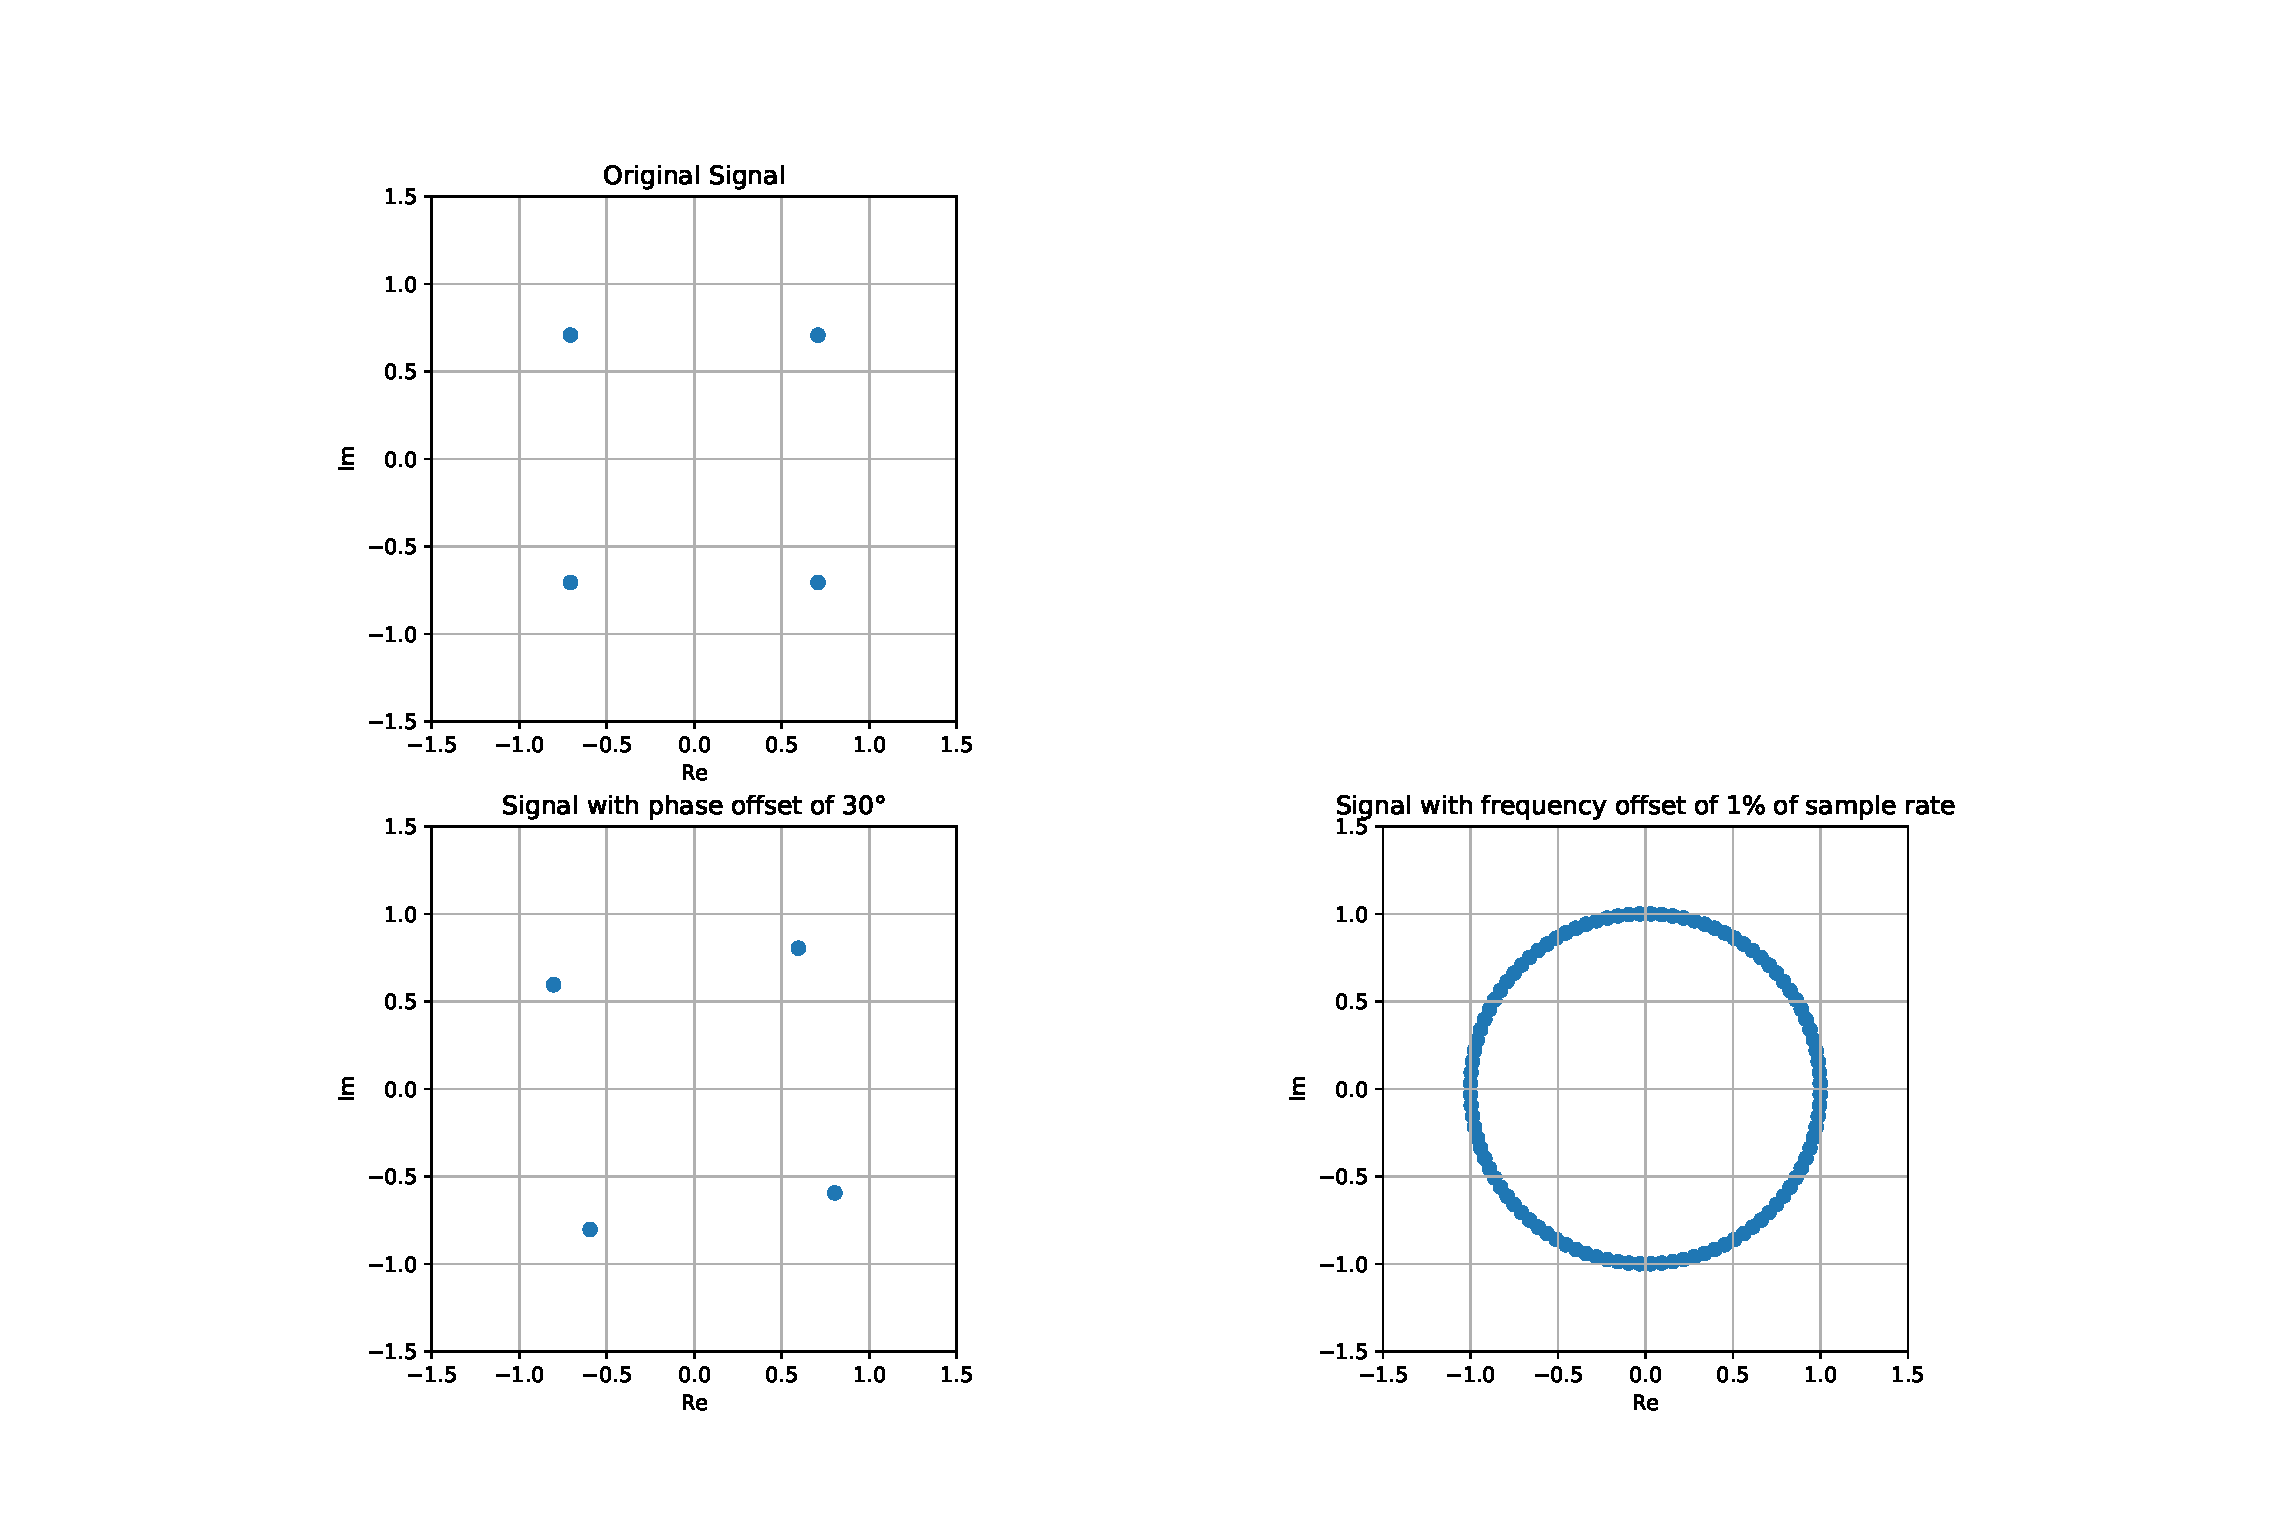
\includegraphics[width=\textwidth]{demo_phase_freq_offset}
  \caption{\code{PhaseFrequencyOffset} demo scatter plots of the original signal and signals with 30° phase offset and 1\% of sample rate frequency offset}
  \label{fig:demo_phase_freq_offset}
\end{figure}

\subsection{Delay Impairment}

The \code{VariableFractionalDelay} module delays the input signal by a specified (and potentially fractional) number of samples.

\noindent Module properties:
\begin{itemize}
  \item \code{max\_delay} (samples): The maximum delay
  \item \code{init\_state}: The initial value to fill in the circular buffer that holds the samples (default=0).
\end{itemize}

The module interpolates the input signal to obtain new samples at non-integer sampling intervals. The only available interpolation method currently is \emph{linear} interpolation. The delay can vary with each invocation of the module (specified by the \code{delay} argument in the \code{\_\_call\_\_()} function). This allows to create a delay profile say, for example, in a triangle or sawtooth shape. The maximum value of the delay is specified using \code{max\_delay}. Delay values greater than the maximum are clipped to the maximum.

The module has a circular buffer of size $\code{max\_delay}+1$ that holds the previous samples, from which it can then compute the interpolation, to obtain the output sequence.

\autoref{lst:demo_delay_offset} shows a demo of this module, using IPython. A QPSK signal is delayed by 1 sample and both the original and delayed signals are plotted for comparison. \autoref{fig:demo_delay_offset} shows the resulting plot. Note in this case the delay offset is fixed to 1 sample, but in general, it can vary in each call to the module.

\begin{python}[label={lst:demo_delay_offset},caption={\code{VariableFractionalDelay} demo}]
  In [17]: import matplotlib.pyplot as plt
    ...: import numpy as np
    ...:
    ...: import sksdr
    ...:
    ...: # Create a delay offset object
    ...: vfd = sksdr.VariableFractionalDelay(max_delay=2)
    ...:
    ...: # Generate random data symbols and apply QPSK modulation
    ...: ints = np.random.randint(0, 4, 10000)
    ...: bits = sksdr.x2binlist(ints, 2)
    ...: psk = sksdr.PSKModulator(sksdr.QPSK, [0, 1, 3, 2], 1.0, np.pi/4)
    ...: mod_sig = psk.modulate(bits)
    ...:
    ...: # Interpolate by 4 and filter with RRC tx filter
    ...: interp = sksdr.FirInterpolator(4, sksdr.rrc(4, 0.5, 10))
    ...: _, tx_sig = interp(mod_sig)
    ...:
    ...: # Apply a delay offset of 1 sample
    ...: tx_sig_off = vfd(tx_sig, 1)
    ...:
    ...: plt.plot(tx_sig.real[:100], '.-', label='Original signal')
    ...: plt.plot(tx_sig_off.real[:100], '.-', label='Delayed signal (1 sample)')
    ...: plt.title('Delayed signal impairment demo')
    ...: plt.grid()
    ...: plt.legend()
    ...: plt.show()
\end{python}

\begin{figure}[H]
  \centering
  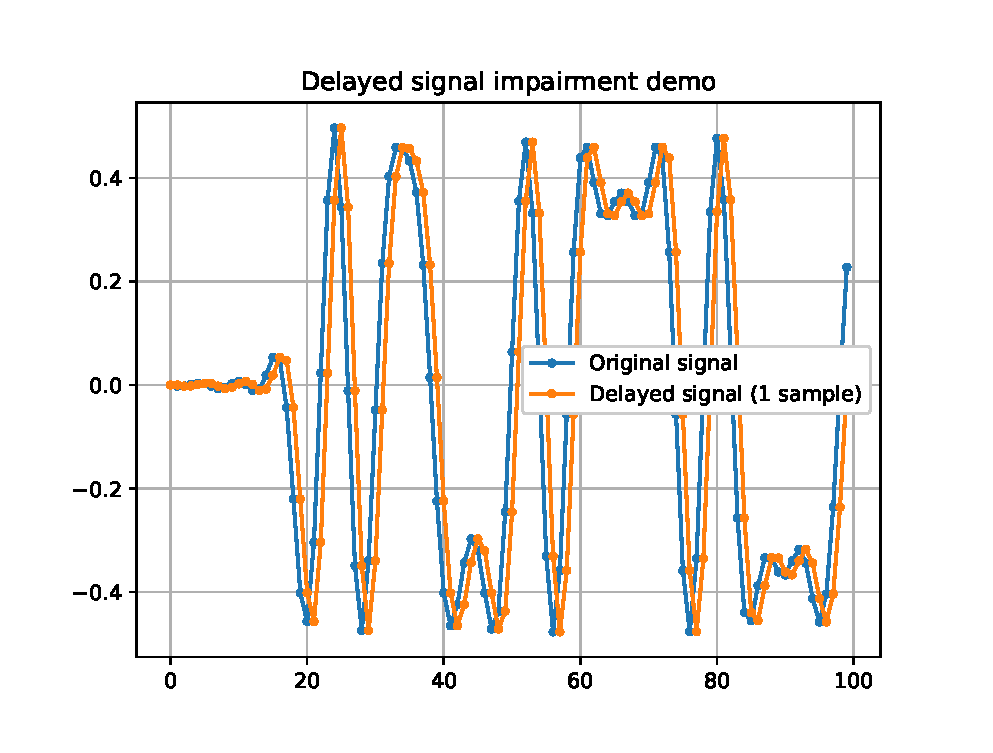
\includegraphics[width=0.75\textwidth]{demo_delay_offset}
  \caption{\code{VariableFractionalDelay} demo plot of the original signal and the delayed signal}
  \label{fig:demo_delay_offset}
\end{figure}

%%%%%%%%%%%%%%%%%%%%%%%%%%%%%%%%%%%%%%%%%%%%%%%%%%%%%%%%%%%%%%%%%%%%%%%%%%%%%%%
\section{Scrambling/Descrambling}

\subsection{Scrambler}

The \code{Scrambler} module scrambles an input signal using a \emph{linear feedback shift register} (LFSR).

\noindent Module properties:
\begin{itemize}
  \item \code{poly}: On/off state for each switch
  \item \code{init\_state}: Initial values of the registers
\end{itemize}

Scrambling is necessary to ensure a signal doesn't contain long sequences of 0's or 1's, which can jeopardize the performance of various blocks, such as the ZCTED discussed in \autoref{sect:timing_error_detector}. \autoref{fig:scrambler_diagram} shows the operation of the Scrambler.

\begin{figure}
\centering
\begin{tikzpicture} [circuit ee IEC,
                     small circuit symbols,
                     every info/.style={font=\footnotesize},
                     set make contact graphic= var make contact IEC graphic,]

\matrix (m1) [row sep=10mm, column sep=10mm]
{
  %--------------------------------------------------------------------
  \node[coordinate] (m00) {}; &
  \node[coordinate] (m01) {}; &
  \node[dspnodeopen,dsp/label=above] (m02) {$y(n)$}; \\
  %--------------------------------------------------------------------
  \node[dspnodeopen,dsp/label=above] (m10) {$x(n)$}; &
  \node[dspadder] (m11) {}; &
  \node[dspsquare] (m12) {1}; &
  \node[dspsquare] (m13) {2}; &
  \node[coordinate] (m14) {}; &
  \node[coordinate] (m15) {}; &
  \node[dspsquare, inner xsep=1mm] (m16) {$M-1$}; &
  \node[dspsquare] (m17) {$M$}; \\
  %--------------------------------------------------------------------
  \node[coordinate] (m20) {}; &
  \node[coordinate] (m21) {}; &
  \node[coordinate] (m22) {}; &
  \node[coordinate] (m23) {}; &
  \node[coordinate] (m24) {}; &
  \node[coordinate] (m25) {}; &
  \node[coordinate] (m26) {}; &
  \node[coordinate] (m27) {}; \\
  %--------------------------------------------------------------------
  \node[coordinate] (m30) {}; &
  \node[coordinate] (m31) {}; &
  \node[dspadder] (m32) {}; &
  \node[dspadder] (m33) {}; &
  \node[coordinate] (m34) {}; &
  \node[coordinate] (m35) {}; &
  \node[dspadder] (m36) {}; &
  \node[coordinate] (m37) {}; \\
};

% Draw connections

\begin{scope}[start chain]
  \chainin (m10);
  \chainin (m11) [join=by dspconn];
  \chainin (m12) [join=by dspconn];
  \chainin (m13) [join=by dspconn];
  \chainin (m14) [join=by dspconn];
  \chainin (m15) [join=by dashed];
  \chainin (m16) [join=by dspconn];
  \chainin (m17) [join=by dspconn];
\end{scope}

\begin{scope}[start chain]
  \chainin (m11);
  \chainin (m01) [join=by dspline];
  \chainin (m02) [join=by dspconn];
\end{scope}

\begin{scope}[start chain]
  \chainin (m37) [join=by dspline];
  \chainin (m36) [join=by dspconn];
  \chainin (m35) [join=by dspconn];
  \chainin (m34) [join=by dashed];
  \chainin (m33) [join=by dspconn];
  \chainin (m32) [join=by dspconn];
  \chainin (m31) [join=by dspline];
  \chainin (m11) [join=by dspconn];
\end{scope}

\draw (m12) to[make contact={near end,info'={$p_1$}}] (m22);
\draw[dspconn] (m22) to (m32);
\draw (m13) to[make contact={near end,info'={$p_2$}}] (m23);
\draw[dspconn] (m23) to (m33);
\draw (m16) to[make contact={near end,info'={$p_{m-1}$}}] (m26);
\draw[dspconn] (m26) to (m36);
\draw (m17) to[make contact={near end,info'={$p_m$}}] (m27);
\draw[dspline] (m27) to (m37);

\end{tikzpicture}
\caption{Scrambler block diagram}
\label{fig:scrambler_diagram}
\end{figure}

At each time step, the input causes the contents of the registers to shift sequentially. Notice that the output for a particular bit depends solely on the $M$ previous bits (excluding the first $N$ bits that will also depend on the initial conditions, where $N$ is the size of the shift register).

\subsection{Descrambler}

The \code{Descrambler} module is used to retrieve the original bit sequence, given an input sequence that's been scrambled using the \code{Scrambler} module.

\noindent Module properties:
\begin{itemize}
  \item \code{poly}: On/off states of the switches
  \item \code{init\_state}: Initial values of the registers
\end{itemize}

\autoref{fig:descrambler_diagram} shows the operation of the Descrambler.

\begin{figure}
\centering
\begin{tikzpicture} [circuit ee IEC,
                     small circuit symbols,
                     every info/.style={font=\footnotesize},
                     set make contact graphic= var make contact IEC graphic,]

\matrix (m1) [row sep=10mm, column sep=10mm]
{
  %--------------------------------------------------------------------
  \node[dspnodeopen,dsp/label=above] (m00) {$x(n)$}; &
  \node[dspnodefull] (m01) {}; &
  \node[dspsquare] (m02) {1}; &
  \node[dspsquare] (m03) {2}; &
  \node[coordinate] (m04) {}; &
  \node[coordinate] (m05) {}; &
  \node[dspsquare, inner xsep=1mm] (m06) {$M-1$}; &
  \node[dspsquare] (m07) {$M$}; \\
  %--------------------------------------------------------------------
  \node[coordinate] (m10) {}; &
  \node[coordinate] (m11) {}; &
  \node[coordinate] (m12) {}; &
  \node[coordinate] (m13) {}; &
  \node[coordinate] (m14) {}; &
  \node[coordinate] (m15) {}; &
  \node[coordinate] (m16) {}; &
  \node[coordinate] (m17) {}; \\
  %--------------------------------------------------------------------
  \node[coordinate] (m20) {}; &
  \node[dspadder,label={above right:$+$},label={below right:$-$}] (m21) {}; &
  \node[dspadder] (m22) {}; &
  \node[dspadder] (m23) {}; &
  \node[coordinate] (m24) {}; &
  \node[coordinate] (m25) {}; &
  \node[dspadder] (m26) {}; &
  \node[coordinate] (m27) {}; \\
  %--------------------------------------------------------------------
  \node[coordinate] (m30) {}; &
  \node[coordinate] (m31) {}; &
  \node[dspnodeopen,dsp/label=above] (m32) {$y(n)$}; \\
};

% Draw connections

 \begin{scope}[start chain]
  \chainin (m00);
  \chainin (m01) [join=by dspline];
  \chainin (m02) [join=by dspconn];
  \chainin (m03) [join=by dspconn];
  \chainin (m04) [join=by dspconn];
  \chainin (m05) [join=by dashed];
  \chainin (m06) [join=by dspconn];
  \chainin (m07) [join=by dspconn];
\end{scope}

\begin{scope}[start chain]
  \chainin (m01);
  \chainin (m21) [join=by dspconn];
  \chainin (m31) [join=by dspline];
  \chainin (m32) [join=by dspconn];
\end{scope}

\begin{scope}[start chain]
  \chainin (m27) [join=by dspline];
  \chainin (m26) [join=by dspconn];
  \chainin (m25) [join=by dspconn];
  \chainin (m24) [join=by dashed];
  \chainin (m23) [join=by dspconn];
  \chainin (m22) [join=by dspconn];
  \chainin (m21) [join=by dspconn];
\end{scope}

\draw (m02) to[make contact={near end,info'={$p_1$}}] (m12);
\draw[dspconn] (m12) to (m22);
\draw (m03) to[make contact={near end,info'={$p_2$}}] (m13);
\draw[dspconn] (m13) to (m23);
\draw (m06) to[make contact={near end,info'={$p_{m-1}$}}] (m16);
\draw[dspconn] (m16) to (m26);
\draw (m07) to[make contact={near end,info'={$p_m$}}] (m17);
\draw[dspline] (m17) to (m27);

\end{tikzpicture}
\caption{Descrambler block diagram}
\label{fig:descrambler_diagram}
\end{figure}

At each time step, the input causes the contents of the registers to shift sequentially. Similarly to the Scramber, the output for a particular bit depends solely on the $M$ previous bits (excluding the first $N$ bits that will also depend on the initial conditions, where $N$ is the size of the shift register).

In both modules, the \code{init\_state} list size must be equal to the \code{poly} list size - 1. The Descrambler \code{poly} and \code{init\_state} must be the same as the ones used in the corresponding Scrambler.

\subsection{Example}

\autoref{lst:scrambling_example} shows an application example of this module, using the IPython console. A stream of bits is scrambler and then descrambled. The descrambled bit sequence is identical to the input bit sequence.
\begin{python}[label={lst:scrambling_example},caption={Scrambling and Descrambling example}]
  In [4]: import sksdr
  ...: scrambler = sksdr.Scrambler([1, 0, 1, 1, 0], [0,1,1,])
  ...: descrambler = sksdr.Descrambler([1, 0, 1, 1, 0], [0,1,1,])
  ...: print('Initiated scrambler with ' + repr(scrambler))
  ...: in_bits = np.random.randint(0, 2, 100)
  ...: scrambled_bits = scrambler(in_bits)
  ...: descrambled_bits = descrambler(scrambled_bits)
  ...: print('Original bits: ' + repr(in_bits))
  ...: print('Scrambled bits: ' + repr(scrambled_bits))
  ...: print('Descrambled bits: ' + repr(descrambled_bits))
Initiated scrambler with Scrambler(poly=[1, 0, 1, 1, 0], init_state=[0, 1, 1])
Original bits: array([
      0, 1, 1, 1, 1, 1, 1, 0, 0, 0, 0, 1, 1, 0, 0, 0, 0, 1, 0, 0, 1, 0,
      1, 0, 0, 1, 0, 0, 0, 0, 0, 1, 1, 0, 1, 1, 0, 1, 0, 1, 1, 0, 0, 0,
      1, 0, 1, 1, 0, 1, 0, 1, 0, 0, 1, 1, 1, 0, 1, 1, 0, 1, 0, 0, 0, 1,
      1, 0, 0, 0, 0, 1, 1, 0, 1, 0, 0, 0, 1, 1, 0, 0, 0, 1, 0, 0, 0, 1,
      0, 1, 0, 1, 1, 0, 0, 0, 1, 0, 0, 1])
Scrambled bits: array([
      0, 0, 1, 1, 0, 1, 0, 1, 1, 1, 0, 1, 0, 1, 1, 1, 0, 1, 1, 1, 1, 0,
      1, 1, 1, 1, 0, 0, 1, 0, 1, 0, 0, 1, 1, 0, 0, 0, 0, 1, 1, 1, 0, 0,
      0, 0, 1, 1, 1, 1, 0, 1, 1, 1, 1, 1, 1, 0, 1, 0, 1, 0, 1, 1, 1, 1,
      1, 0, 0, 1, 0, 0, 0, 0, 1, 0, 1, 1, 0, 1, 1, 1, 0, 1, 1, 1, 0, 1,
      1, 0, 0, 0, 1, 0, 1, 1, 0, 0, 1, 1])
Descrambled bits: array([
      0, 1, 1, 1, 1, 1, 1, 0, 0, 0, 0, 1, 1, 0, 0, 0, 0, 1, 0, 0, 1, 0,
      1, 0, 0, 1, 0, 0, 0, 0, 0, 1, 1, 0, 1, 1, 0, 1, 0, 1, 1, 0, 0, 0,
      1, 0, 1, 1, 0, 1, 0, 1, 0, 0, 1, 1, 1, 0, 1, 1, 0, 1, 0, 0, 0, 1,
      1, 0, 0, 0, 0, 1, 1, 0, 1, 0, 0, 0, 1, 1, 0, 0, 0, 1, 0, 0, 0, 1,
      0, 1, 0, 1, 1, 0, 0, 0, 1, 0, 0, 1])
\end{python}

%%%%%%%%%%%%%%%%%%%%%%%%%%%%%%%%%%%%%%%%%%%%%%%%%%%%%%%%%%%%%%%%%%%%%%%%%%%%%%%
\section{Forward Error Correcting Algorithms}
Forward error correction (FEC) is a technique used for detecting and possibly correcting errors in data transmission over unreliable communication channels \cite{wikipedia_fec}. This is achieved by adding redundant information to the message, that is then used by the receiver in the error detection process. FEC allows the receiver correct errors without needing to request re-transmission of data, but at the cost of a higher channel bandwidth. This is specially useful for systems in which re-transmissions are not viable due to latency issues for example.
The maximum proportion of errors or missing bits that can be corrected is determined by the design of the ECC, so different forward error correcting codes are suitable for different conditions.

\subsection{Hamming(7,4) Code}

The Hamming(7,4) was developed in the SKSDR library as way of demonstration and experimentation. The idea is that the library can be extended in the future with other algorithms including for example convolutional codes like Viterbi coding.

\noindent Module properties:
\begin{itemize}
  \item \code{ntotal}: The total number of bits (data + parity) (currently fixed as 7)
  \item \code{ndata}: The number of data bits (currently fixed as 4)
\end{itemize}

Hamming(7,4) is a linear error-correcting code that encodes four bits of data into seven bits by adding three parity bits \cite{wikipedia_hamming}. The algorithm can correct any single-bit error, or detect all single-bit and two-bit errors. Because Hamming codes are linear codes, they can be computed efficiently using matrices. Two Hamming matrices can be defined, the code \emph{generator matrix} G and the \emph{parity-check matrix} H:
\begin{equation}
\mathbf{G^T} := \begin{pmatrix}
  1 & 1 & 0 & 1 \\
  1 & 0 & 1 & 1 \\
  1 & 0 & 0 & 0 \\
  0 & 1 & 1 & 1 \\
  0 & 1 & 0 & 0 \\
  0 & 0 & 1 & 0 \\
  0 & 0 & 0 & 1 \\
 \end{pmatrix}, \qquad \mathbf{H} := \begin{pmatrix}
  1 & 0 & 1 & 0 & 1 & 0 & 1 \\
  0 & 1 & 1 & 0 & 0 & 1 & 1 \\
  0 & 0 & 0 & 1 & 1 & 1 & 1 \\
 \end{pmatrix}.
\end{equation}

One can be derived from the other. For example, if the generator matrix for an [n,k]-code is in standard form:
\begin{equation}
  G = \begin{bmatrix} I_k | P \end{bmatrix}
\end{equation}
then the parity check matrix is given by
\begin{equation}
  H = \begin{bmatrix} -P^{\top} | I_{n-k} \end{bmatrix}
\end{equation}
because
\begin{equation}
G H^{\top} = P-P = 0
\end{equation}

\autoref{fig:hamming_74} illustrates the relationship between the data bits and the parity bits, showing which data bits are covered by each of the parity bits.

\begin{figure}[H]
  \centering
  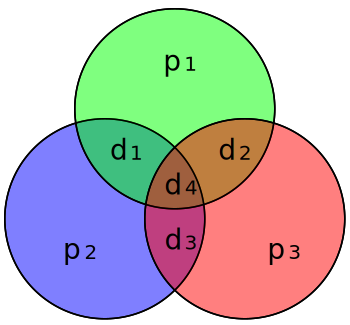
\includegraphics[width=0.25\textwidth]{hamming_74}
  \caption{Venn diagram showing the relationship between data bits and parity bits in the Hamming(7,4) code [\citeauthor{image:hamming74_venn_diagram}]}
  \label{fig:hamming_74}
\end{figure}

\autoref{lst:hamming_74} shows an application example of this module, using the IPython console. A stream of bits is encoded and an error is introduced in one bit. The stream is then decoded and the error is corrected. The output bit sequence is identical to the input bit sequence.

\begin{python}[label={lst:hamming_74},caption={Hamming(7,4) example}]
In [46]: import sksdr
  ...: h74 = sksdr.Hamming(7, 4)
  ...: msg = [1, 0, 0, 1]
  ...: send = h74.encode(msg)
  ...: # Introduce an error by inverting one of the data or parity bits
  ...: send[2] = send[2] ^ 1
  ...: recv = h74.decode(send)
  ...: recv
  ...:
Out[46]: (array([1, 0, 0, 1]), array([2]))
\end{python}
